%!TeX root = ../main.tex

% ==========================================
% CHAPTER 4: EXPERIMENTAL RESULTS AND COMPARISON
% ==========================================
\chapter{Experimental Results and Comparison}
\label{ch:results}

Chapters~\ref{Ch:Kinematic} and~\ref{ch:architecture} established, respectively, the kinematic models of the two platforms and the software architecture required to deploy them fairly within the ROS~2 Nav2 stack. This chapter presents the experimental validation of that architecture and the quantitative comparison between the differential PMB2 and the holonomic OmniBase. The evaluation spans the two navigation pipelines that motivate this work: directed waypoint navigation across three topological challenges, and autonomous frontier-based exploration of an unknown domestic environment. Each scenario was repeated for five iterations per base, and all spatial quantities were computed offline from absolute Ground Truth poses, so that the observed differences can be attributed to the underlying kinematics and the resulting navigation strategies rather than to onboard estimation noise. The chapter first describes the simulation environments and experimental protocols (Section~\ref{sec:exp-setup}) and the evaluation metrics together with their methodological caveats (Section~\ref{sec:eval-metrics}); it then reports the waypoint and exploration results (Sections~\ref{sec:wp-results} and~\ref{sec:expl-results}) and closes with a cross-paradigm synthesis (Section~\ref{sec:comparative-discussion}).

\section{Experimental Setup}
\label{sec:exp-setup}

The experimental campaigns were conducted entirely in simulation, relying on the Gazebo Classic worlds and the deterministic launch infrastructure detailed in Chapter~\ref{ch:architecture}. This section introduces the two simulation scenarios (Section~\ref{subsec:sim-scenarios}) and the two experimental protocols used to benchmark the platforms: directed waypoint navigation (Section~\ref{subsec:wp-protocol}) and autonomous exploration (Section~\ref{subsec:expl-protocol}).

\subsection{Simulation Scenarios}
\label{subsec:sim-scenarios}

Two distinct Gazebo Classic worlds were employed (Figure~\ref{fig:sim-worlds}), each tailored to one of the two navigation pipelines. Both environments were instrumented with the \texttt{gazebo\_ros\_state} plugin introduced in Section~\ref{subsec:simulation_gt}, which publishes the absolute pose of the robot at 50~Hz and provides the Ground Truth reference used throughout the offline analysis.

The directed waypoint-navigation campaign was executed in the PAL Robotics  \\ \texttt{small\_office} world, a structured indoor environment. As detailed in Section~\ref{subsec:simulation_gt}, this stock world was adapted for benchmarking by adjusting the lighting, removing overhanging desks that produced blind collisions above the LiDAR plane, and populating the space with static human models to emulate a realistic, cluttered office. Its regular geometry makes it well suited to controlled and repeatable path-following tests, since the three waypoint routes (Section~\ref{subsec:wp-protocol}) can be arranged to isolate specific navigational challenges---a straight corridor, a sharp corner, and a densely obstructed passage.

The autonomous-exploration campaign was instead conducted in the \texttt{home} world, a realistic domestic apartment comprising multiple connected rooms. In contrast to the office, this environment was deliberately left unaltered in order to preserve a highly complex and representative scenario. Because the exploration task requires the robot to incrementally discover an initially unknown map, the larger scale and irregular room topology of the apartment provide a demanding setting in which to compare the two kinematics under simultaneous localisation and mapping.

\begin{figure}[H]
    \centering
    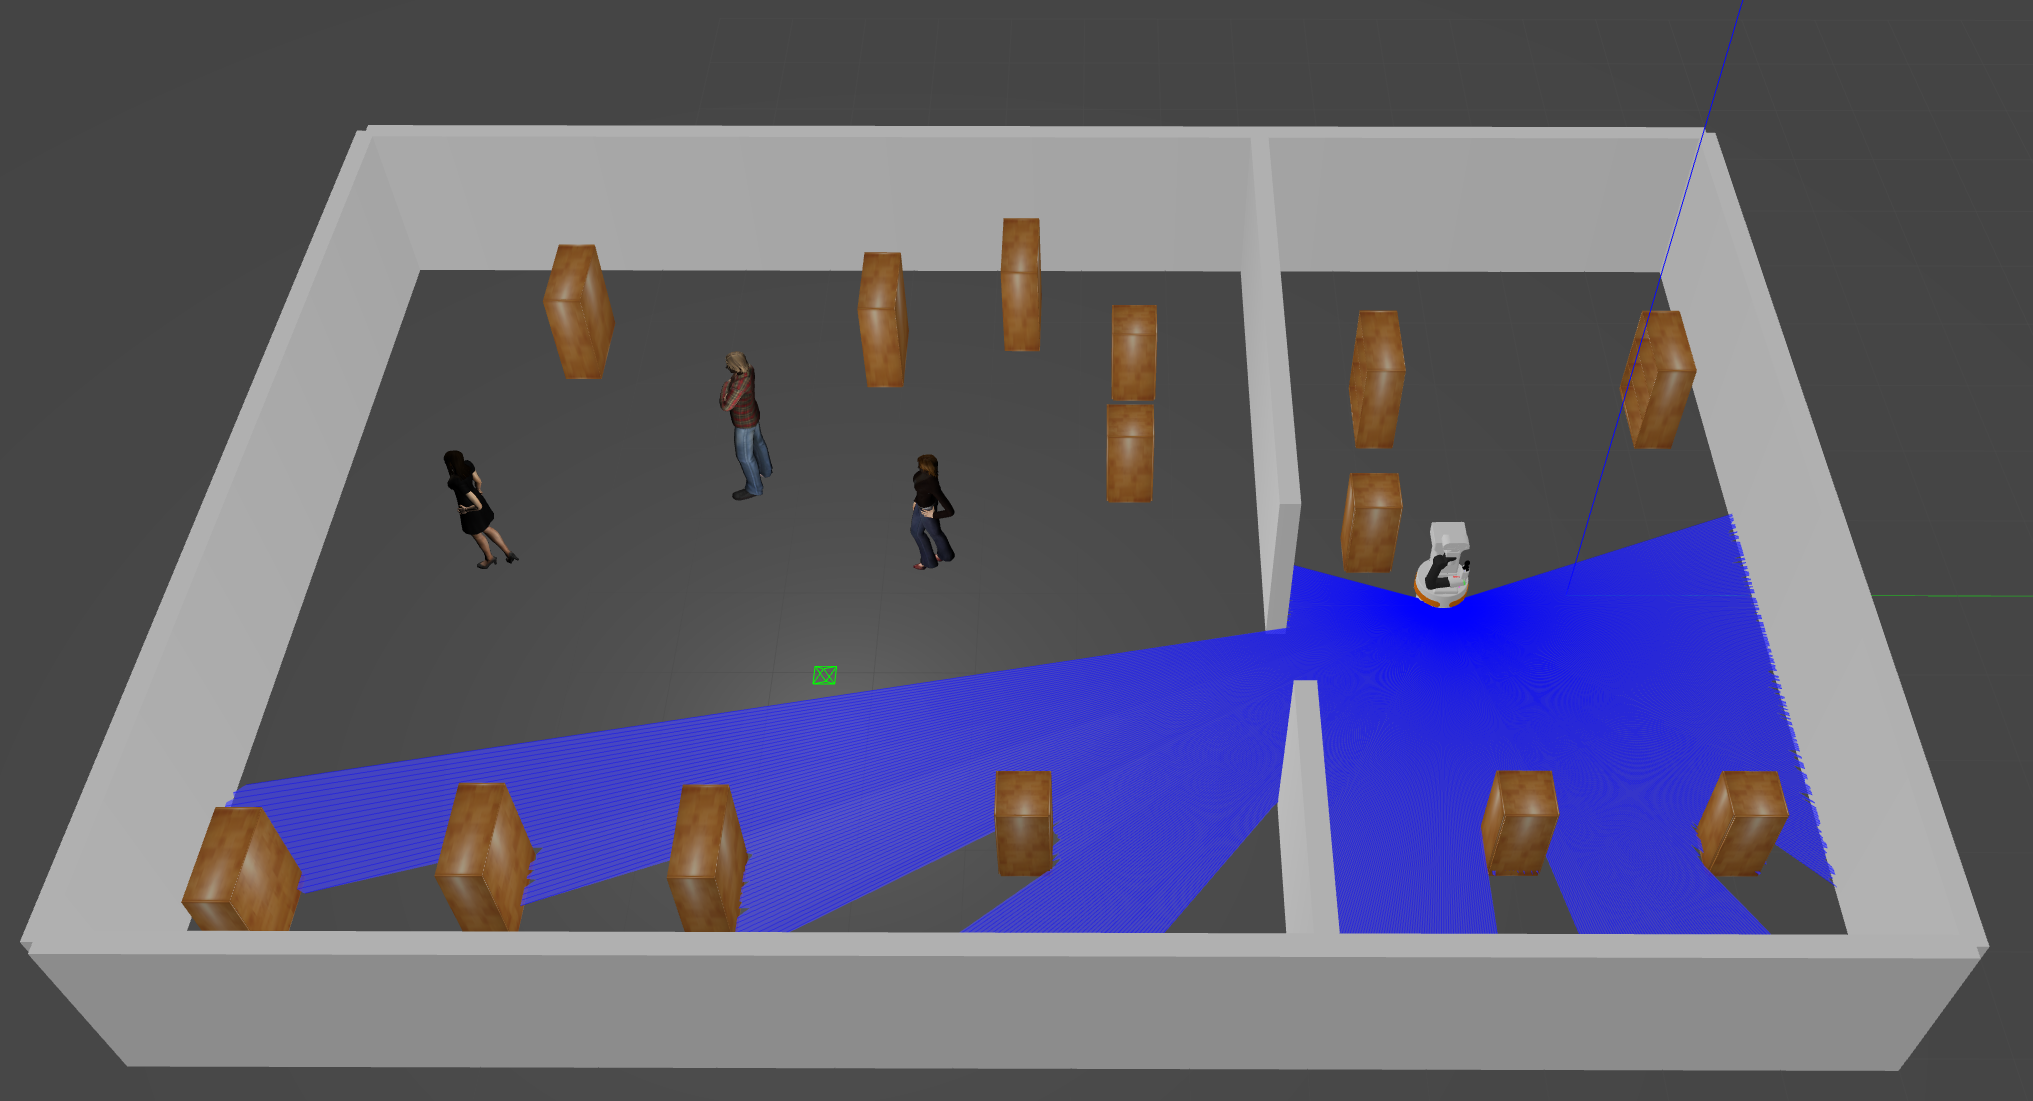
\includegraphics[width=0.49\textwidth]{images/Ch4/Small_office_diff.png}
    \hfill
    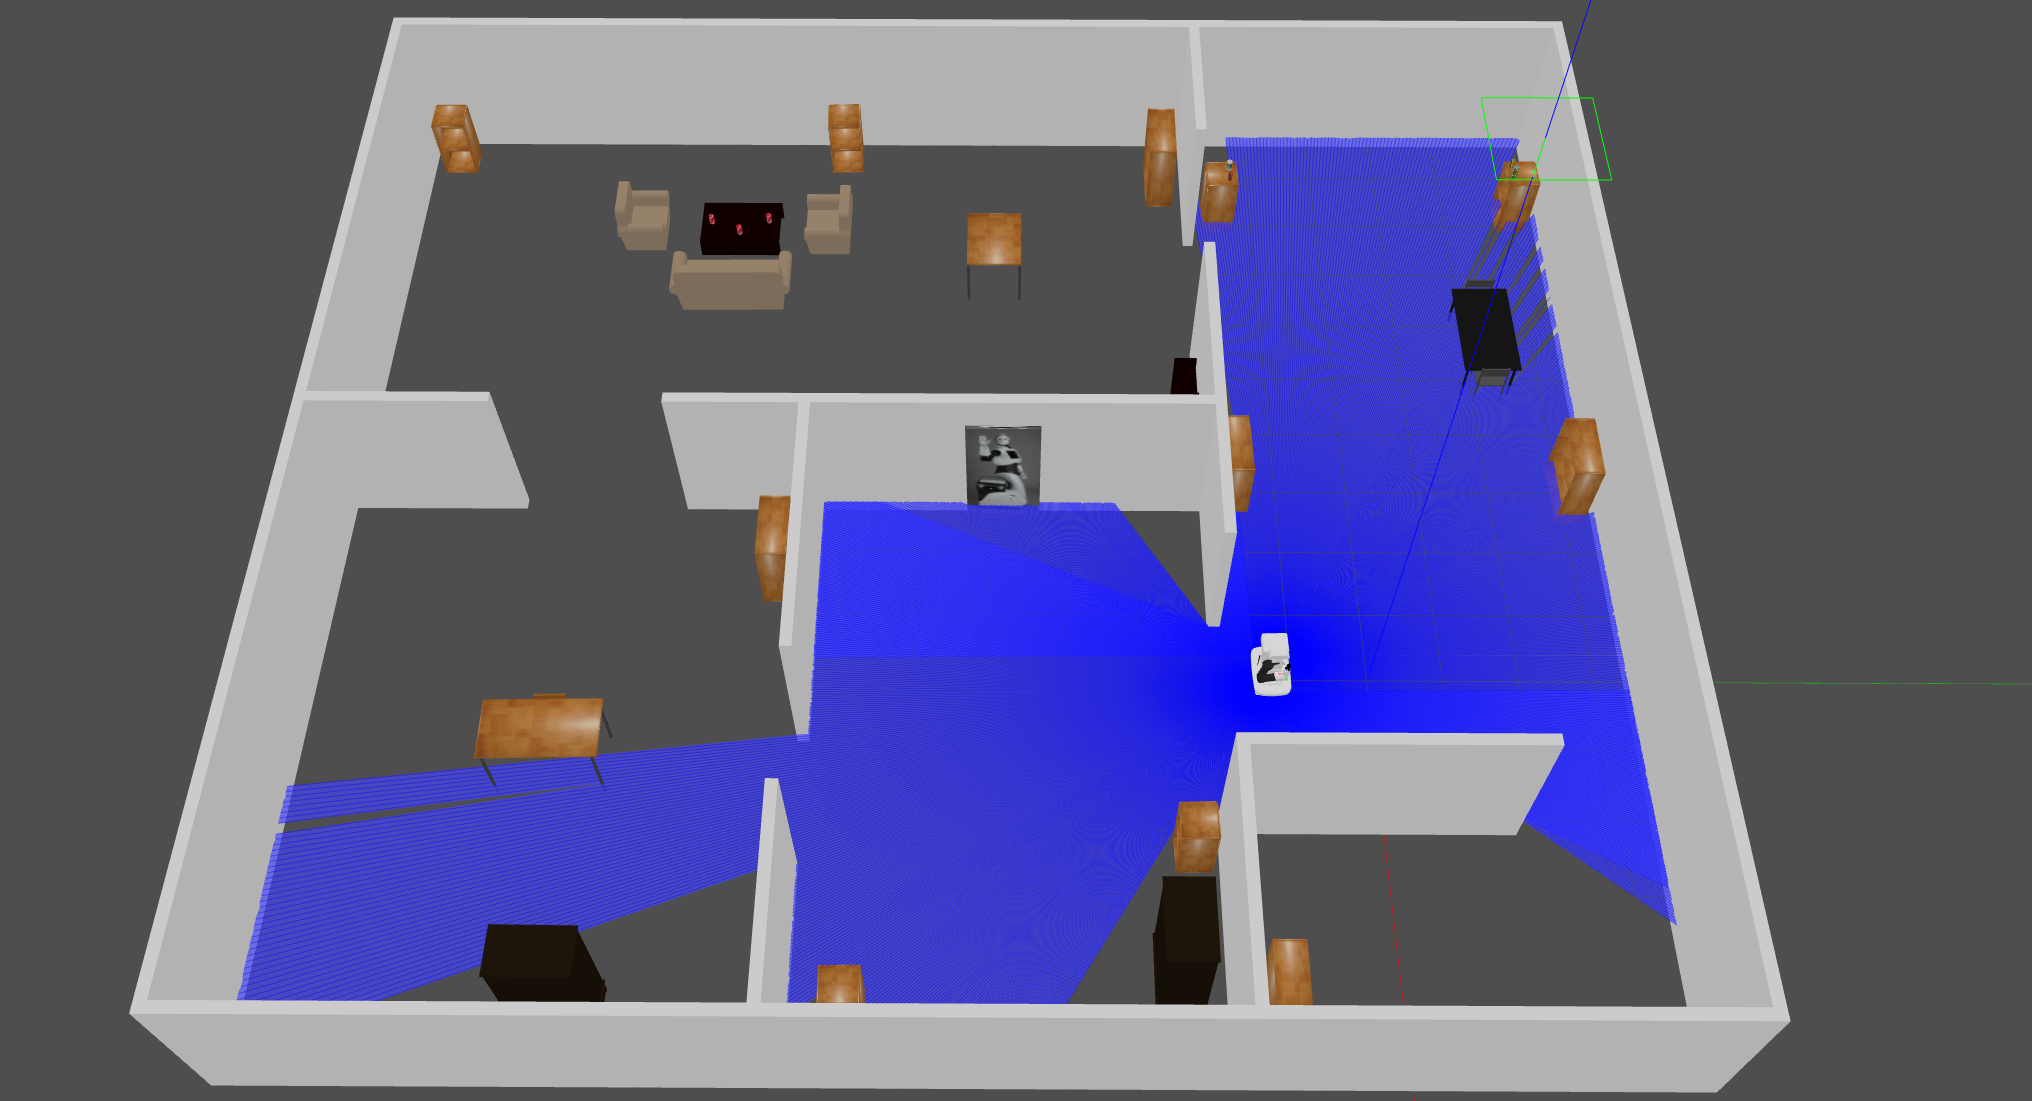
\includegraphics[width=0.49\textwidth]{images/Ch4/Home_omni.png}
    \caption{The two Gazebo Classic simulation environments. Left: the modified \texttt{small\_office} world used for the waypoint-navigation campaign, populated with static obstacles and human models. Right: the unaltered \texttt{home} apartment used for the autonomous-exploration campaign.}
    \label{fig:sim-worlds}
\end{figure}

\subsection{Waypoint Navigation Protocol}
\label{subsec:wp-protocol}

The first pipeline evaluates directed point-to-point navigation on a previously mapped environment. The robot was commanded to traverse an ordered sequence of poses through the Nav2 \texttt{NavigateThroughPoses} action, dispatched from a custom driver node built on the \\ \texttt{nav2\_simple\_commander} API (the driver and the Ground~Truth logging node are documented in Appendix~\ref{app:results_scripts}). Unlike a series of independent \texttt{NavigateToPose} goals, this action plans a single continuous path through all the intermediate poses without requiring the robot to stop at each one. Consequently, the intermediate waypoints behave as positional via-points that the trajectory is only required to approach within tolerance, leaving the platform free to smooth the path---most notably by cutting corners---rather than pausing and re-orienting at every pose. Moreover, only the orientation of the final pose is enforced: the headings assigned to the intermediate waypoints are not actively pursued. This behaviour is central to the correct interpretation of the positioning and orientation errors and is discussed further in Section~\ref{sec:eval-metrics}.

Three routes of increasing difficulty were designed within the \texttt{small\_office} world, each isolating a distinct navigational challenge. Their exact coordinates are reported in Appendix~B.

\textbf{Path~A --- Straight Corridor.} A two-waypoint route consisting of a single rectilinear segment, approximately $13$~m long, running along a straight corridor of the office (Figure~\ref{fig:hallway_traj}). With no turns or obstacles, this path isolates pure path-following and steady-state velocity behaviour, and serves as the baseline against which the two kinematics are first compared.

\textbf{Path~B --- Sharp Corner.} A four-waypoint route describing an ``L''-shaped trajectory: a $1.5$~m segment followed by a sharp $90^{\circ}$ turn and a further $1.3$~m segment, for a total reference length of $2.8$~m. This deliberately short route stresses the platforms' response to an abrupt change of direction, contrasting the in-place rotation required by the differential drive with the lateral strafing available to the holonomic one.

\textbf{Path~C --- Cluttered Obstacle Course.} An eleven-waypoint route, approximately $25.9$~m long, winding through the populated office and passing in close proximity to two static human models. By repeatedly forcing the global planner to compute paths through narrow, obstructed passages, this route most severely stresses the planning stack and is expected to expose the differences in navigation robustness between the two bases.

All three routes begin at the spawn pose (waypoint~$0$), so that every run starts from the precise coordinates enforced by the deterministic initialisation routine of Section~\ref{subsec: Deterministic Init}. The positioning error at this first waypoint is therefore null by construction and is disregarded when interpreting the results, which focus instead on the intermediate waypoints and the final goal. Each route was executed five times per base, yielding a total of $30$ waypoint-navigation runs ($2$ bases $\times$ $3$ routes $\times$ $5$ repetitions). During every run, the absolute Ground~Truth pose was logged at $50$~Hz together with the velocity commands issued by the navigation stack; all metrics and figures were then computed offline over the \emph{active navigation window}---from the instant the first waypoint becomes active until the sequence completes---so as to exclude the initial postural settling at spawn and any idle time after arrival.
\begin{figure}[H]
    \centering
    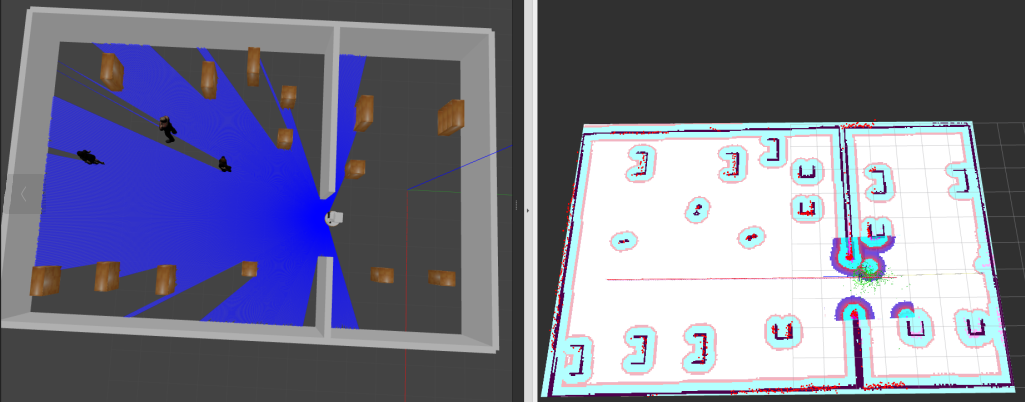
\includegraphics[width=1\textwidth]{images/Ch4/Zoom_Setup_simulazione_hallway.png} 
    \caption{Path~A --- Straight Corridor during simulation}
    \label{fig:hallway_traj}
\end{figure}


\subsection{Autonomous Exploration Protocol}
\label{subsec:expl-protocol}

The second pipeline evaluates autonomous exploration of an initially unknown environment. In contrast to the waypoint campaign, no map is provided in advance: the robot incrementally builds an occupancy grid on-line through \texttt{slam\_toolbox} while Nav2 drives it towards a succession of self-selected goals. This setting exercises the full navigation loop---simultaneous mapping, localisation, global planning, and local control---and is therefore the more demanding test of how each kinematic model copes with a realistic domestic space (the \texttt{home} world of Section~\ref{subsec:sim-scenarios}; Figure~\ref{fig:aut-exp sim}).

Exploration is driven by a custom frontier-based node (documented in Appendix~\ref{app: autonomous expl node}), originally developed during a prior internship and substantially re-instrumented for this thesis to guarantee deterministic and fair comparisons. At each iteration the node analyses the live occupancy grid published by SLAM and identifies the \emph{frontiers}, i.e.\ the cells lying on the boundary between explored free space and still-unknown regions. A single frontier is then selected according to a configurable, deterministic policy and dispatched to Nav2 as a navigation goal, with its orientation set towards the unexplored area so that the robot arrives already facing the region to be scanned. The cycle repeats until the number of residual frontier cells falls below a fixed threshold, at which point the map is considered complete and the robot returns to its starting position.

Deploying a naive frontier explorer on the two platforms would, however, conflate genuine kinematic differences with incidental planner failures. Three heuristics were therefore introduced to keep the comparison fair and repeatable:
\begin{itemize}
    \item \textbf{Goal retraction from unknown boundaries.} A frontier cell lies exactly on the free/unknown border; as the robot approaches it, the laser frequently reveals a wall just beyond the previous sensor horizon, whose inflation then covers the goal and makes the previously valid target unreachable, triggering spurious recovery behaviours. Each goal is therefore pulled back by a fixed distance along the frontier-to-robot direction, so that it falls in already-confirmed free space while the robot still advances towards, and scans, the frontier.
    \item \textbf{Wall-clearance filtering.} Frontiers lying closer than a minimum clearance to an obstacle are discarded a priori, preventing the planner from being sent towards goals trapped inside the costmap inflation layer.
    \item \textbf{Dynamic goal blacklisting.} Any goal rejected or aborted by the planner is added to a blacklist and excluded, together with a surrounding radius, from subsequent selections, which avoids endless recovery loops around a single problematic point.
\end{itemize}

To ensure that both bases were driven by exactly the same exploration logic, all of these parameters were held identical across the two platforms: a nearest-frontier selection policy, a minimum wall clearance of $0.55$~m, a goal retraction of $0.40$~m, a blacklist radius of $1.0$~m, a completion threshold of $10$ residual frontier cells, and a per-goal navigation timeout of $20$~s. Consequently, any difference in the exploration behaviour reflects the underlying kinematics and the response of the shared Nav2 stack, rather than a divergence in the exploration strategy itself.

As in the waypoint campaign, the exploration was repeated five times per base---for a total of $10$ runs---to characterise run-to-run variability, since the interaction between planner, incremental SLAM updates, and goal selection makes each run slightly different even under a deterministic policy. Throughout each run the absolute Ground~Truth pose was logged alongside the SLAM pose estimate and the commanded velocities; the SLAM localisation error, and the map-to-world frame alignment required to compute it fairly for the two bases, are discussed in Section~\ref{sec:eval-metrics}. All metrics were again evaluated over the active exploration window, from the first frontier goal until the completion criterion is met.

\begin{figure}[H]
     \centering
     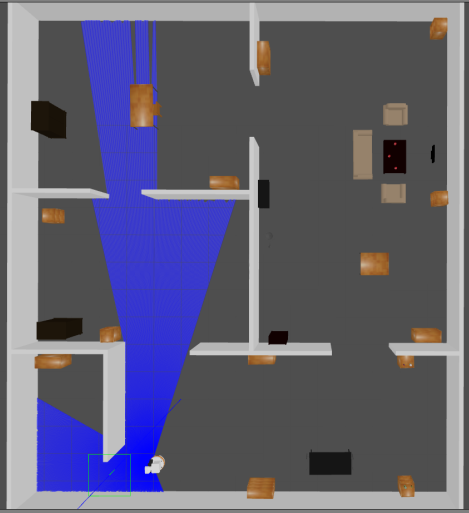
\includegraphics[width=0.45\textwidth]{images/Ch4/zoom_gazebo_aut_exp.png}
     \hfill
     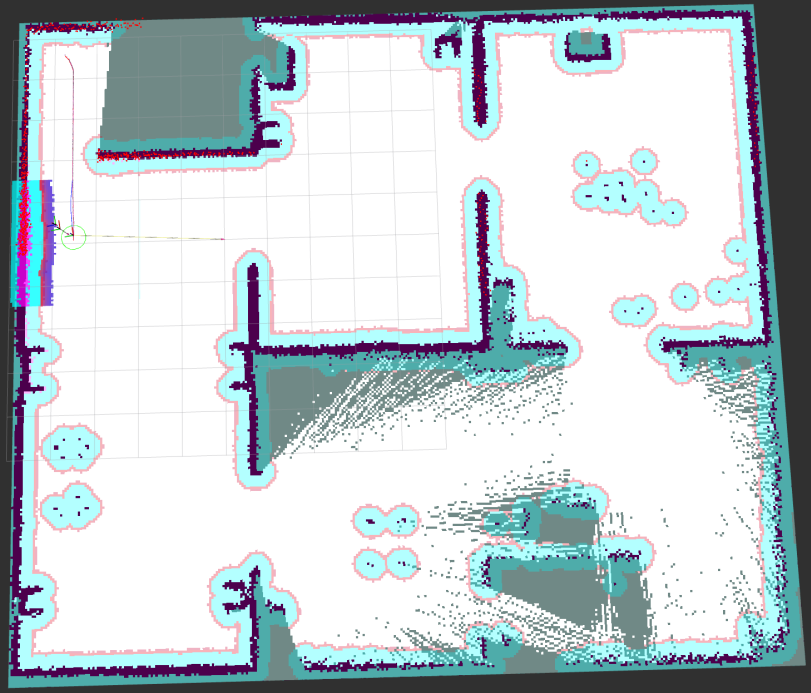
\includegraphics[width=0.5\textwidth]{images/Ch4/zoom_rviz_aut_exp.png}
     \caption{Autonomous Exploration Simulation. Left: Gazebo environment. Right: RViz environment.}
     \label{fig:aut-exp sim}
\end{figure}


\section{Evaluation Metrics}
\label{sec:eval-metrics}

All quantities compared in this chapter were computed offline from the absolute Ground~Truth poses of Section~\ref{subsec:simulation_gt}, not from the robot's own estimate: odometry drifts without bound and AMCL adds model-dependent noise, so evaluating path-following through each base's localisation would confound the kinematic comparison with an estimation artefact. Every metric is evaluated over the active navigation window and, unless stated otherwise, reported as mean $\pm$ standard deviation over the five repetitions of each configuration. The following subsections define the accuracy (Section~\ref{subsec:m-accuracy}), efficiency and motion-quality (Section~\ref{subsec:m-efficiency}), and robustness (Section~\ref{subsec:m-robustness}) metrics, the exploration-specific metrics (Section~\ref{subsec:m-exploration}), and the simulation-fidelity considerations that frame the fairness of the comparison (Section~\ref{subsec:m-fidelity}).

\subsection{Trajectory and Path-Following Accuracy}
\label{subsec:m-accuracy}

The \emph{path length} is the arc length of the Ground~Truth trajectory over the active window; the \emph{reference length} is the sum of the straight segments joining all waypoints. The two need not coincide---cutting corners shortens the path, detouring around obstacles lengthens it---so the reference is a descriptive baseline, not an optimum, and is read together with the tracking error.

The \emph{tracking error} measures how faithfully a base follows the planned trajectory: for each Ground~Truth sample it is the perpendicular distance to the Nav2 global plan (\texttt{/plan}) of the \emph{leg} active at that instant---a leg being the stretch of route between two consecutive waypoints---summarised by its mean, maximum, and root-mean-square. The plan is used as reference---rather than a straight waypoint-to-waypoint line---because it already embeds the planner's \\ obstacle-avoidance detours, so the deviation from it answers the meaningful question of how closely the base executed the path it was actually given. For each leg the reference is the plan published at the start of that leg, reconstructed offline from the recorded rosbag; on the rare legs without an available plan, the analysis falls back to the straight segment and flags the substitution.

The \emph{waypoint positioning error} is the \emph{closest-approach} distance between the trajectory and each waypoint. Because \texttt{NavigateThroughPoses} yields a single fluid trajectory that does not stop at the intermediate poses (Section~\ref{subsec:wp-protocol}), this definition is preferred over the pose sampled at the index switch for three reasons:
\begin{enumerate}
    \item \textbf{Robustness to skipped indices.} A fast base can retire two poses within one feedback cycle, so an intermediate index is never published---as for the OmniBase on Path~B---leaving an index-based rule undefined, whereas the closest approach is always well defined.
    \item \textbf{Honest meaning at pass-through waypoints.} It equals exactly how far the trajectory passed from the point, i.e.\ the corner-cutting distance.
    \item \textbf{Consistency at the goal.} At the final stop it coincides with the final positioning error, free of the timing noise of an arbitrary sampling instant.
\end{enumerate}
The error at the first waypoint, where the robot spawns, is close to zero by construction (up to a small residual reflecting the initial placement) and is not analysed further.

The \emph{orientation error}, evaluated at the point of closest approach, requires care. With \texttt{NavigateThroughPoses} only the final orientation is enforced, so the intermediate waypoint headings are decorative and the error there is measured against a target never pursued; moreover, at a pass-through waypoint the heading equals the instantaneous direction of motion, so a differential base---which must rotate in order to translate---is constantly re-orienting and shows large intermediate errors, while a holonomic base holds a fixed heading while strafing. The intermediate orientation error is therefore read as an indicator of heading stability, and only the error at the final goal, where the heading is genuinely commanded, measures final angular accuracy.

\subsection{Efficiency and Motion Quality}
\label{subsec:m-efficiency}

The \emph{completion time} is the duration of the active window, measured in simulated time, and the \emph{average speed} is the path length divided by it. Relying on simulated time makes the results independent of the simulation's real-time factor (RTF), which was not strictly below unity---on the short Path~B runs it reached $1.02$--$1.21$---and which enforcing \texttt{use\_sim\_time} across the pipeline (Section~\ref{subsec:gpu optimization}) renders irrelevant to the comparison: all nodes share Gazebo's \texttt{/clock}, so durations stay consistent regardless of how fast the simulation ran on the wall clock.

\emph{Motion smoothness} is quantified as the root-mean-square of the commanded acceleration, obtained by numerically differentiating the linear and angular velocity commands issued on \texttt{/cmd\_vel}; a lower value denotes smoother motion. It is computed from the commands, rather than from the Ground~Truth trajectory, so that it reflects the control effort requested by the planner, and it is reported separately as a linear and an angular component (\texttt{smooth\_lin}, \texttt{smooth\_ang}).

Finally, the \emph{lateral usage} is the fraction of the motion performed through the lateral (strafing) velocity component: zero by construction for the differential base, which cannot translate sideways, and positive for the holonomic one, it directly measures how much each platform exploited its available degrees of freedom.

\subsection{Robustness}
\label{subsec:m-robustness}

Navigation robustness is assessed primarily through the \emph{planning failures}: the number of times the global planner failed to produce a valid path, and the corresponding \emph{failure rate}, i.e.\ failures over planning attempts. This is the metric on which the two kinematics differ most sharply, the differential base repeatedly failing to plan around obstacles where the holonomic one does not.

Complementing it, the \emph{recovery behaviours} count the Nav2 recovery actions triggered when normal planning or control stalls---rotating in place (Spin), reversing (BackUp), waiting (Wait), and costmap clearing (ClearCostmap). Costmap clearing is the most frequent around obstacles and, in the Nav2 behaviour tree, is invoked by a planning failure before the next attempt; the spatial location of these clears therefore marks where planning struggled, which motivates the recovery maps shown in the results.

A further quantity, the number of \emph{replans}, is reported only for completeness: replanning is issued periodically at roughly $1$~Hz, so its count scales with run duration rather than with difficulty, and it is treated as a secondary, bookkeeping quantity rather than a headline indicator. All of the above counts were extracted offline from the recorded rosbags by parsing the \texttt{/behavior\_tree\_log} topic and counting each behaviour's activations---a single, uniform source across both pipelines, which also correctly captures one-shot actions such as costmap clearing.

\subsection{Exploration-Specific Metrics}
\label{subsec:m-exploration}

The exploration task is characterised by a dedicated set of metrics, alongside the smoothness, lateral-usage, and robustness quantities already defined, which apply unchanged. The \emph{final mapped area} is the free area of the occupancy grid at the end of the run, and the \emph{exploration time} is the duration of the active exploration window. To compare runs that terminate with slightly different coverage, the \emph{time-to-target} measures the time taken to map a common target area, set to $95\%$ of the smallest final area observed across all runs, so that every run is evaluated at a coverage level all of them attained. Exploration \emph{efficiency} is then expressed both per unit distance (area per metre travelled) and per unit time (area per second).

The \emph{SLAM localisation error} is the distance between the Ground~Truth pose and the pose estimated by \texttt{slam\_toolbox}, summarised by its mean and maximum. Computing it fairly requires aligning the SLAM \texttt{map} frame with the Gazebo \texttt{world} frame, because the two bases operate under different odometric regimes by construction of their simulation plugins: the PMB2 wheel odometry is zeroed at spawn, so its \texttt{map} origin coincides with the spawn pose, whereas the OmniBase is driven by \texttt{gazebo\_ros\_planar\_move}, whose odometry is referenced to the world, so its \texttt{map} origin already coincides with it. Without correction, the PMB2 would exhibit a spurious constant offset---about $1.3$~m, the spawn displacement---that is not a SLAM error. An initial-pose (ATE-style) alignment is therefore estimated from the first valid samples of each run and removed before the error is computed, making the two measurements comparable.

\subsection{Simulation Fidelity and the Fairness of the Comparison}
\label{subsec:m-fidelity}

As anticipated in Section~\ref{subsec:odom tf bridge}, the two bases are actuated differently in simulation, and this asymmetry must be kept in mind when reading the results. The PMB2 is driven through \texttt{ros2\_control}, so its motion follows from an idealised model of the wheel dynamics, whereas the OmniBase is driven by \texttt{gazebo\_ros\_planar\_move}, which imposes the commanded body twist $(v_x, v_y, \omega)$ directly, without any actuation dynamics. As a consequence, the OmniBase follows the velocity commands almost perfectly \emph{by construction}, not because it is inherently a superior platform. The same reasoning applies to the wheel-rotation comparison used in the results: the OmniBase wheel velocities are not measured but reconstructed from the inverse kinematic model of Chapter~\ref{Ch:Kinematic}, whereas the PMB2 wheel rotation is read from the simulator. The comparison nonetheless remains meaningful because both describe an ideal, no-slip rotation---by construction for the OmniBase, and, for the PMB2, effectively so on a flat floor where the simulated wheels barely slip---so the two quantities live in the same idealised kinematic regime rather than reflecting actuation dynamics.

Three implications follow:
\begin{enumerate}
    \item \textbf{Optimistic timing and smoothness.} The holonomic base enjoys a mild optimistic bias on completion time and smoothness, as it executes the acceleration-limited command with no actuation lag; its advantage on these metrics should therefore be read as an upper bound.
    \item \textbf{Understated variance.} Its very low run-to-run variance is partly a plugin effect, and is reported as such rather than claimed as physical stability of the robot.
    \item \textbf{Strategy-level framing.} The comparison is consequently framed at the level of the navigation and planning strategy under different kinematics---the subject of this thesis---rather than as a comparison of physical execution fidelity.
\end{enumerate}
The most trustworthy metrics are thus those independent of actuation fidelity: completion time in simulated units, path shape, the amount of in-place rotation, and lateral usage. For the same reason, the SLAM comparison of Section~\ref{subsec:m-exploration} is best understood as the same SLAM algorithm operating on two different odometric regimes, rather than as a property of the bases in isolation.

\section{Waypoint Navigation Results}
\label{sec:wp-results}

This section reports the results of the waypoint-navigation campaign, presenting the three routes in order of increasing difficulty: the straight corridor (Section~\ref{subsec:res-hallway}), the sharp corner (Section~\ref{subsec:res-angle}), and the cluttered obstacle course (Section~\ref{subsec:res-obstacles}). For each route the two platforms are compared on the metrics defined in Section~\ref{sec:eval-metrics}, aggregated as mean $\pm$ standard deviation over the five repetitions; per-run detail is illustrated using the median run of each base, selected by completion time.

\subsection{Straight Corridor (Path~A)}
\label{subsec:res-hallway}

On the straight corridor both platforms completed all five runs successfully, and neither triggered a single recovery behaviour or planning failure: the route is short and unobstructed, so the navigation stack drives each base to the goal without intervention. Figure~\ref{fig:hallway-traj} shows the Ground~Truth trajectories of all runs, which form a tight bundle along the corridor axis for both bases and confirm the high repeatability of the setup. The aggregate metrics are summarised in Table~\ref{tab:hallway}.

\begin{table}[htbp]
\centering
\caption{Straight corridor (Path~A): aggregate metrics, mean $\pm$ standard deviation over five runs.}
\label{tab:hallway}
\begin{tabular}{lcc}
\toprule
Metric & PMB2 (differential) & OmniBase (holonomic) \\
\midrule
Completion time [s]            & $24.10 \pm 0.52$ & $23.56 \pm 0.14$ \\
Average speed [m/s]            & $0.534 \pm 0.011$ & $0.542 \pm 0.003$ \\
Tracking error, mean [m]      & $0.124 \pm 0.024$ & $0.079 \pm 0.020$ \\
Tracking error, RMS [m]       & $0.147 \pm 0.030$ & $0.100 \pm 0.021$ \\
Goal positioning error [m]    & $0.269 \pm 0.039$ & $0.238 \pm 0.023$ \\
Linear smoothness [m/s$^2$]   & $1.340 \pm 0.058$ & $0.845 \pm 0.081$ \\
Angular smoothness [rad/s$^2$] & $0.614 \pm 0.093$ & $0.611 \pm 0.107$ \\
Lateral usage                  & $0.000 \pm 0.000$ & $0.075 \pm 0.010$ \\
Recoveries / plan failures     & $0$ / $0$ & $0$ / $0$ \\
\bottomrule
\end{tabular}
\end{table}

\begin{figure}[H]
  \centering
  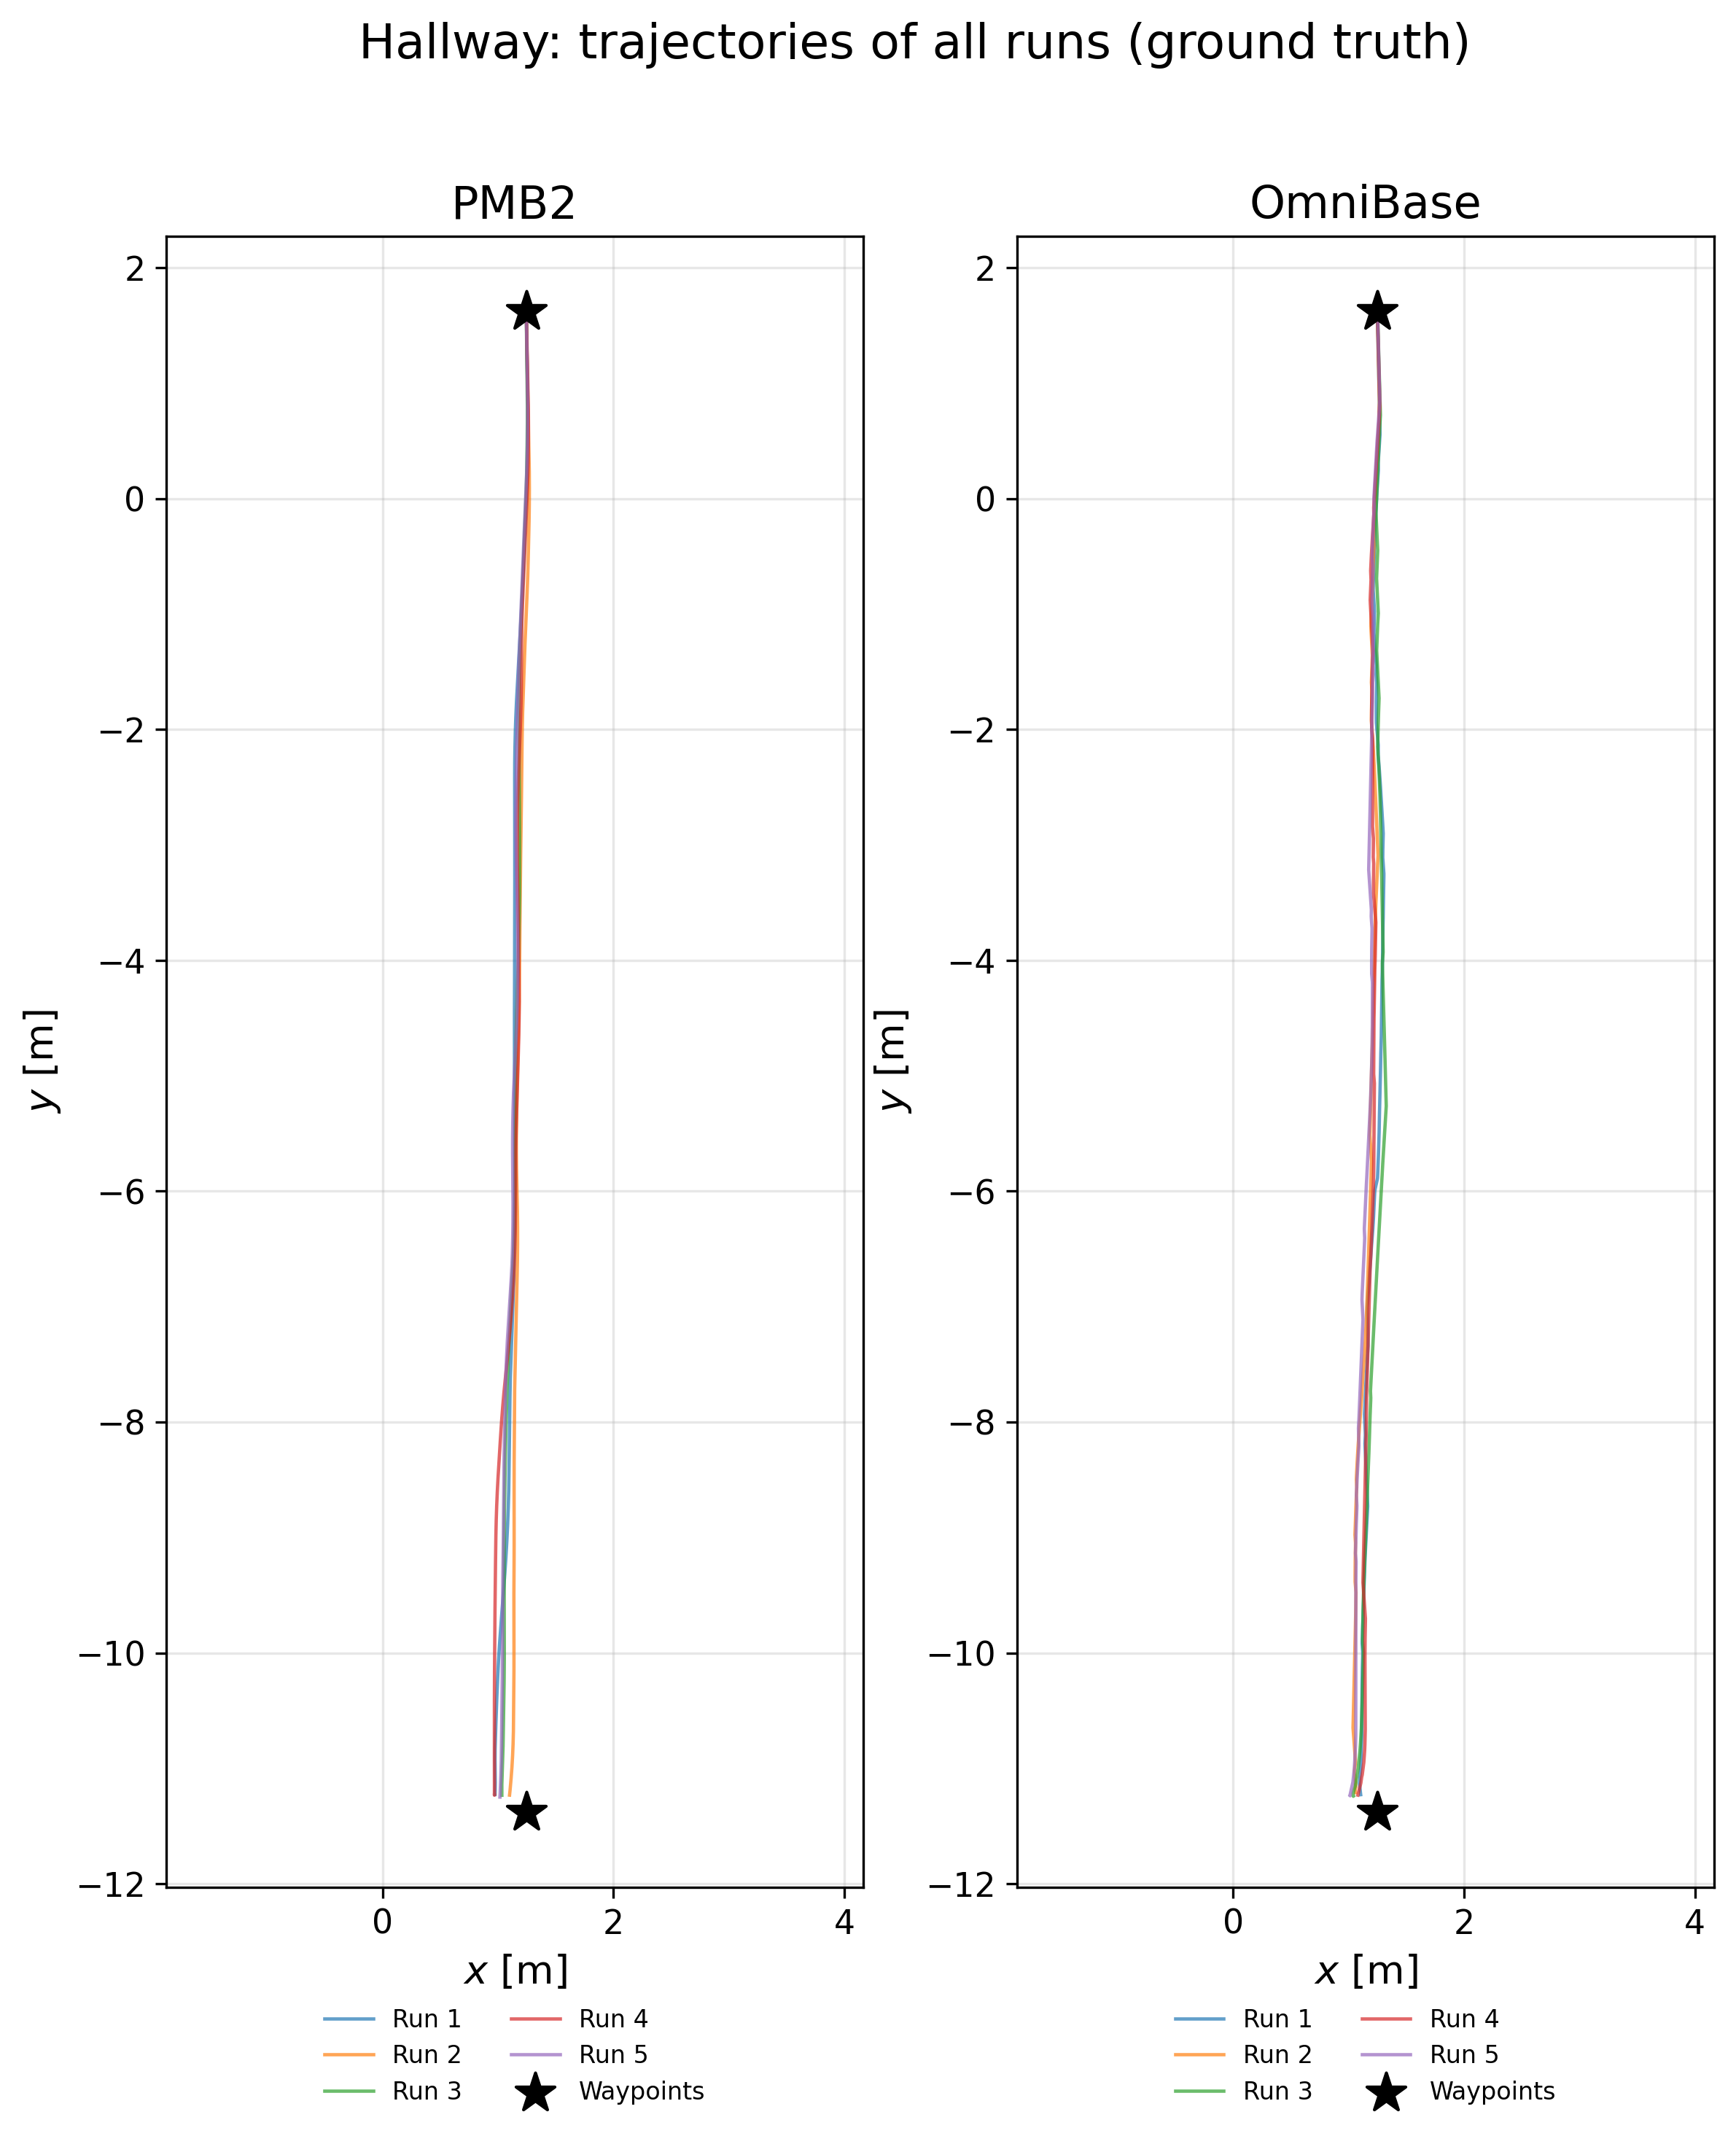
\includegraphics[width=1\textwidth]{images/Ch4/hallway/trajectories_all_Hallway.png}
  \caption{Straight corridor: Ground~Truth trajectories of all five runs per base. Both platforms follow the corridor axis with high repeatability. Stars mark the start (WP0) and the goal (WP1).}
  \label{fig:hallway-traj}
\end{figure}

Although both bases follow the corridor closely, the holonomic OmniBase tracks the planned path more faithfully. Its mean deviation from the Nav2 global plan is about a third smaller than the differential's ($0.079$ against $0.124$~m; RMS $0.100$ against $0.147$~m), and the same ordering holds for the maximum deviation. Figure~\ref{fig:hallway-xtrack} shows that for both platforms the deviation is negligible at the start and grows along the corridor, but the OmniBase keeps it consistently lower, its error curve repeatedly dipping as the base actively returns onto the planned path.

\begin{figure}[H]
  \centering
  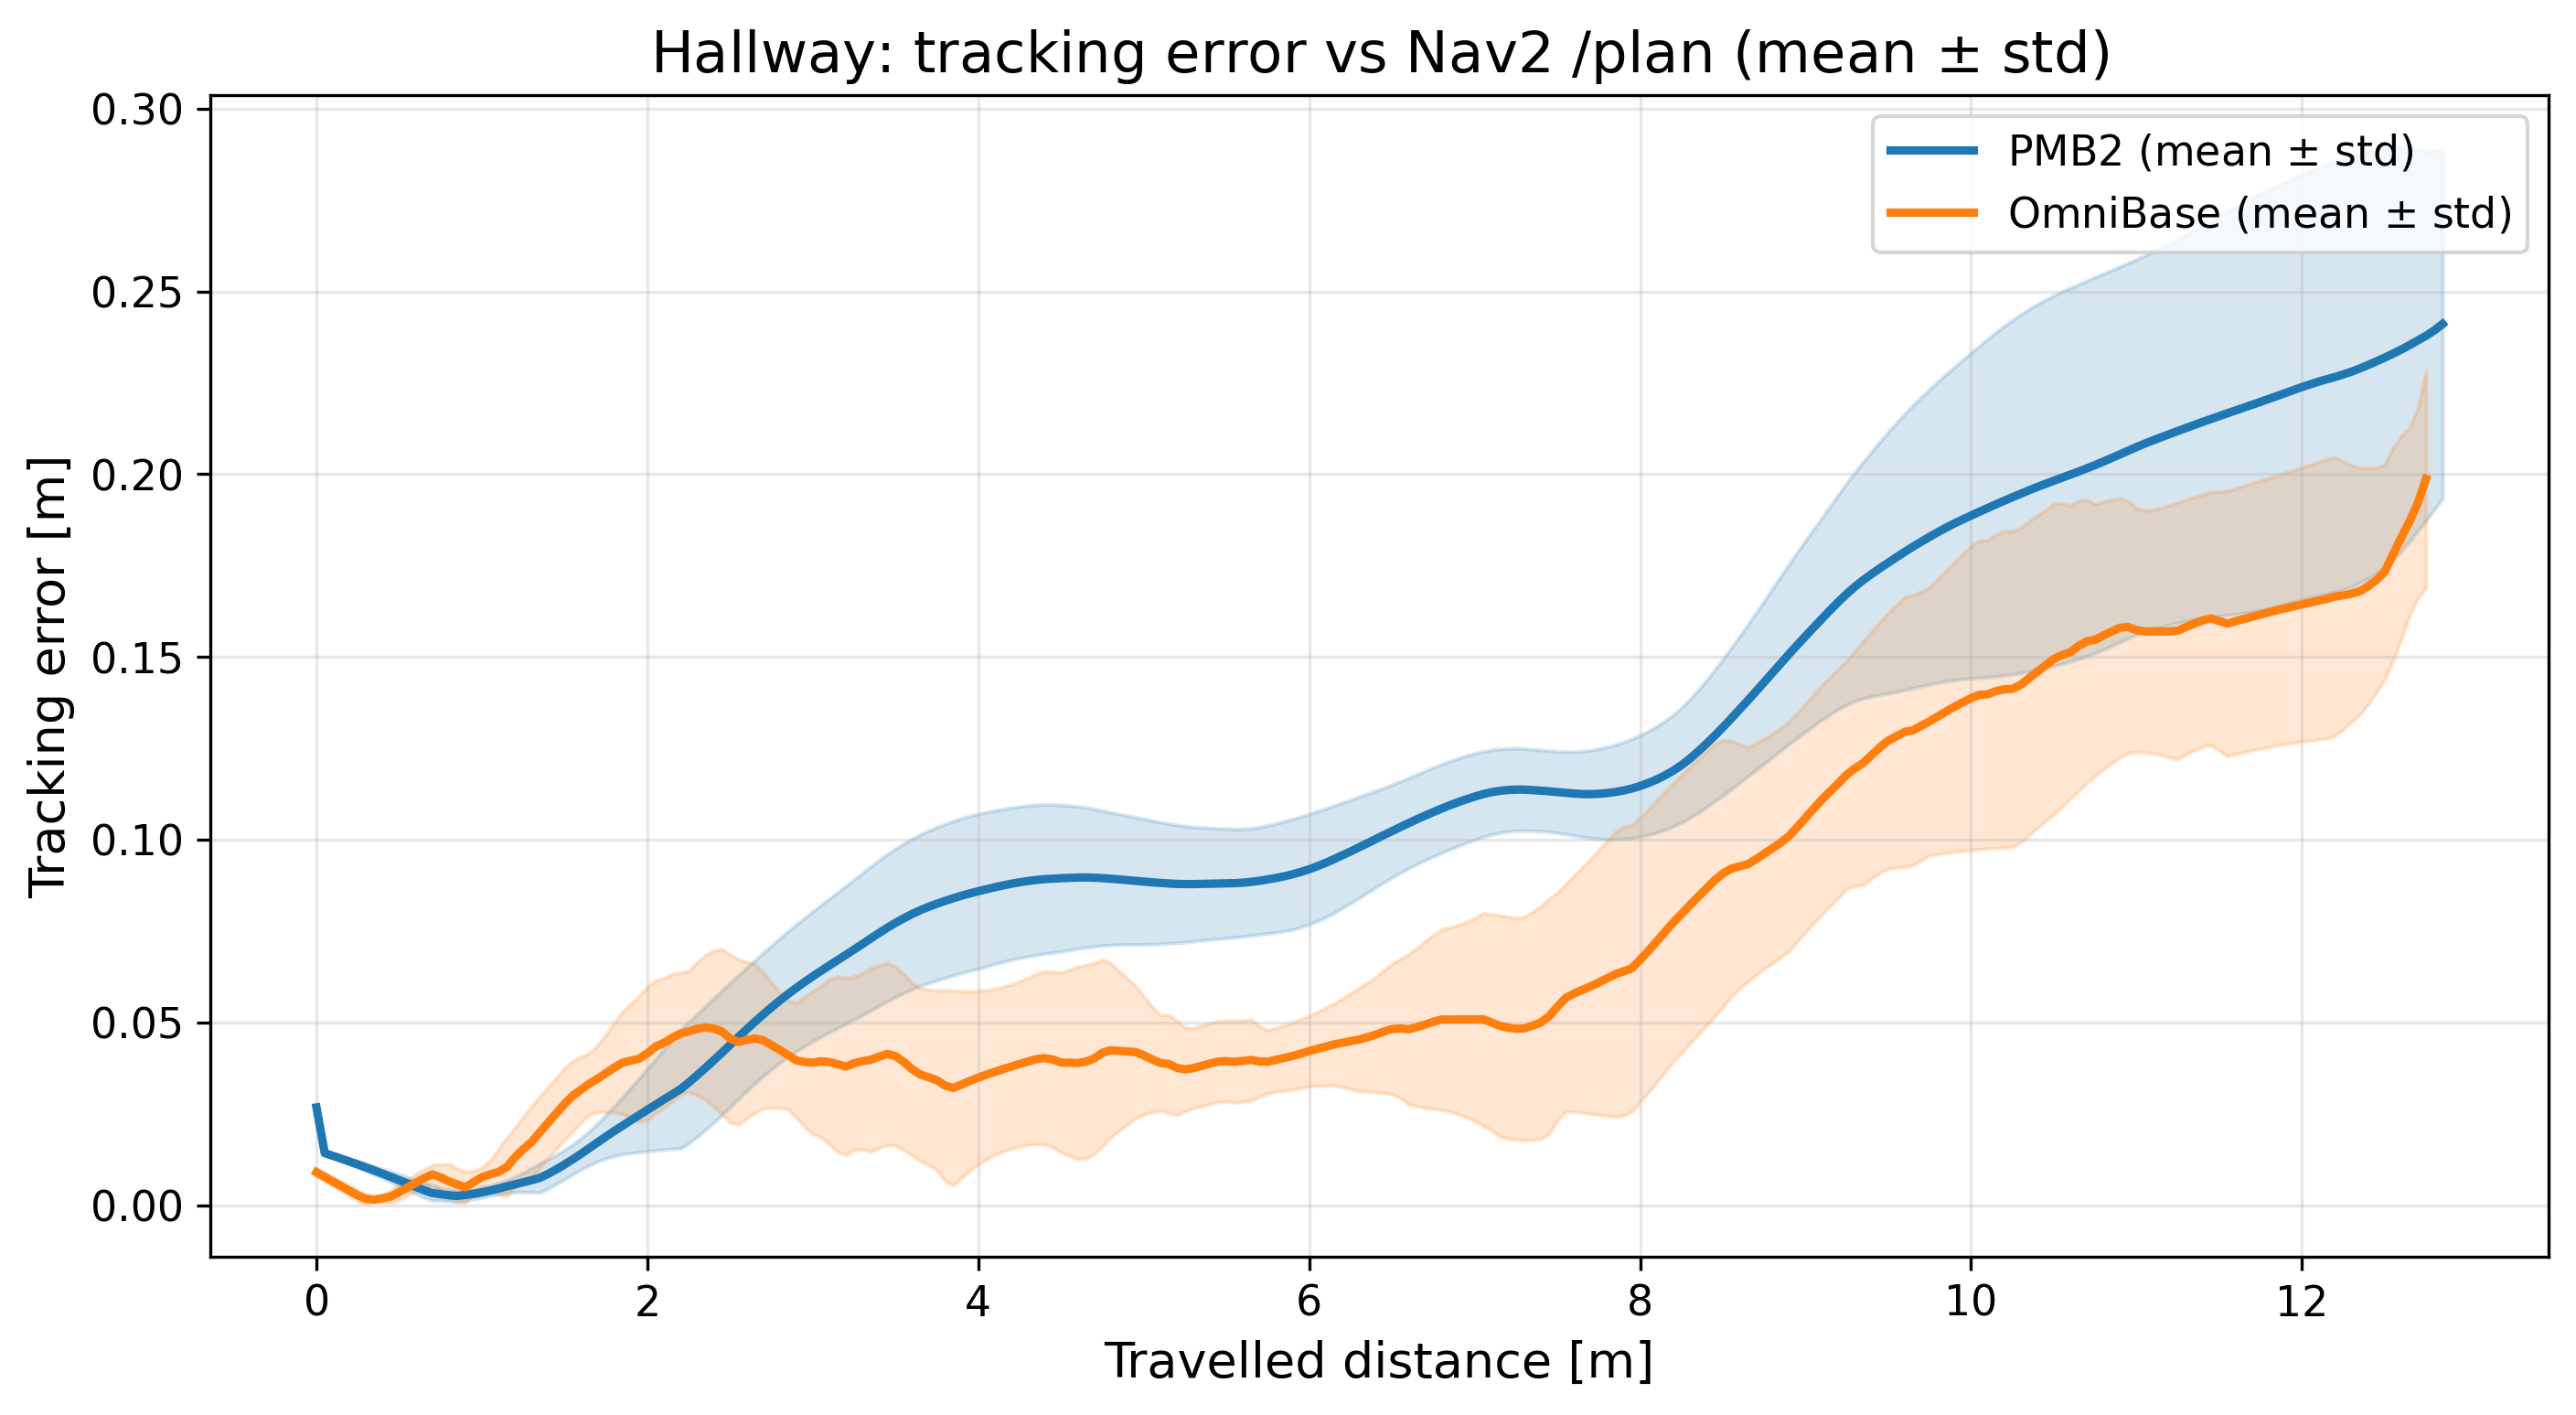
\includegraphics[width=1\textwidth]{images/Ch4/hallway/cross_track_band_Hallway.png}
  \caption{Straight corridor: tracking error against the Nav2 global plan as a function of travelled distance (mean $\pm$ standard deviation over five runs). The deviation grows along the corridor for both bases but remains consistently smaller for the holonomic OmniBase.}
  \label{fig:hallway-xtrack}
\end{figure}

This difference is explained by the commanded velocity profiles of Figure~\ref{fig:hallway-vel}. The OmniBase corrects lateral drift directly, through short pulses of lateral velocity $v_y$ (centre panel)---a capability reflected in a non-zero lateral usage ($0.075$) and structurally unavailable to the differential base, whose $v_y$ is identically zero and which can only realign by adjusting its heading through $\omega_z$. The two controllers, individually tuned, cruise at somewhat different peak forward speeds, yet cover the corridor in comparable time. The OmniBase also commands smoother linear motion (Table~\ref{tab:hallway}, \texttt{smooth\_lin} $0.845$ against $1.340$), a difference to be read in the light of the actuation-fidelity caveat of Section~\ref{subsec:m-fidelity}; the angular smoothness is instead essentially identical, since neither base turns appreciably on a straight path.

\begin{figure}[H]
  \centering
  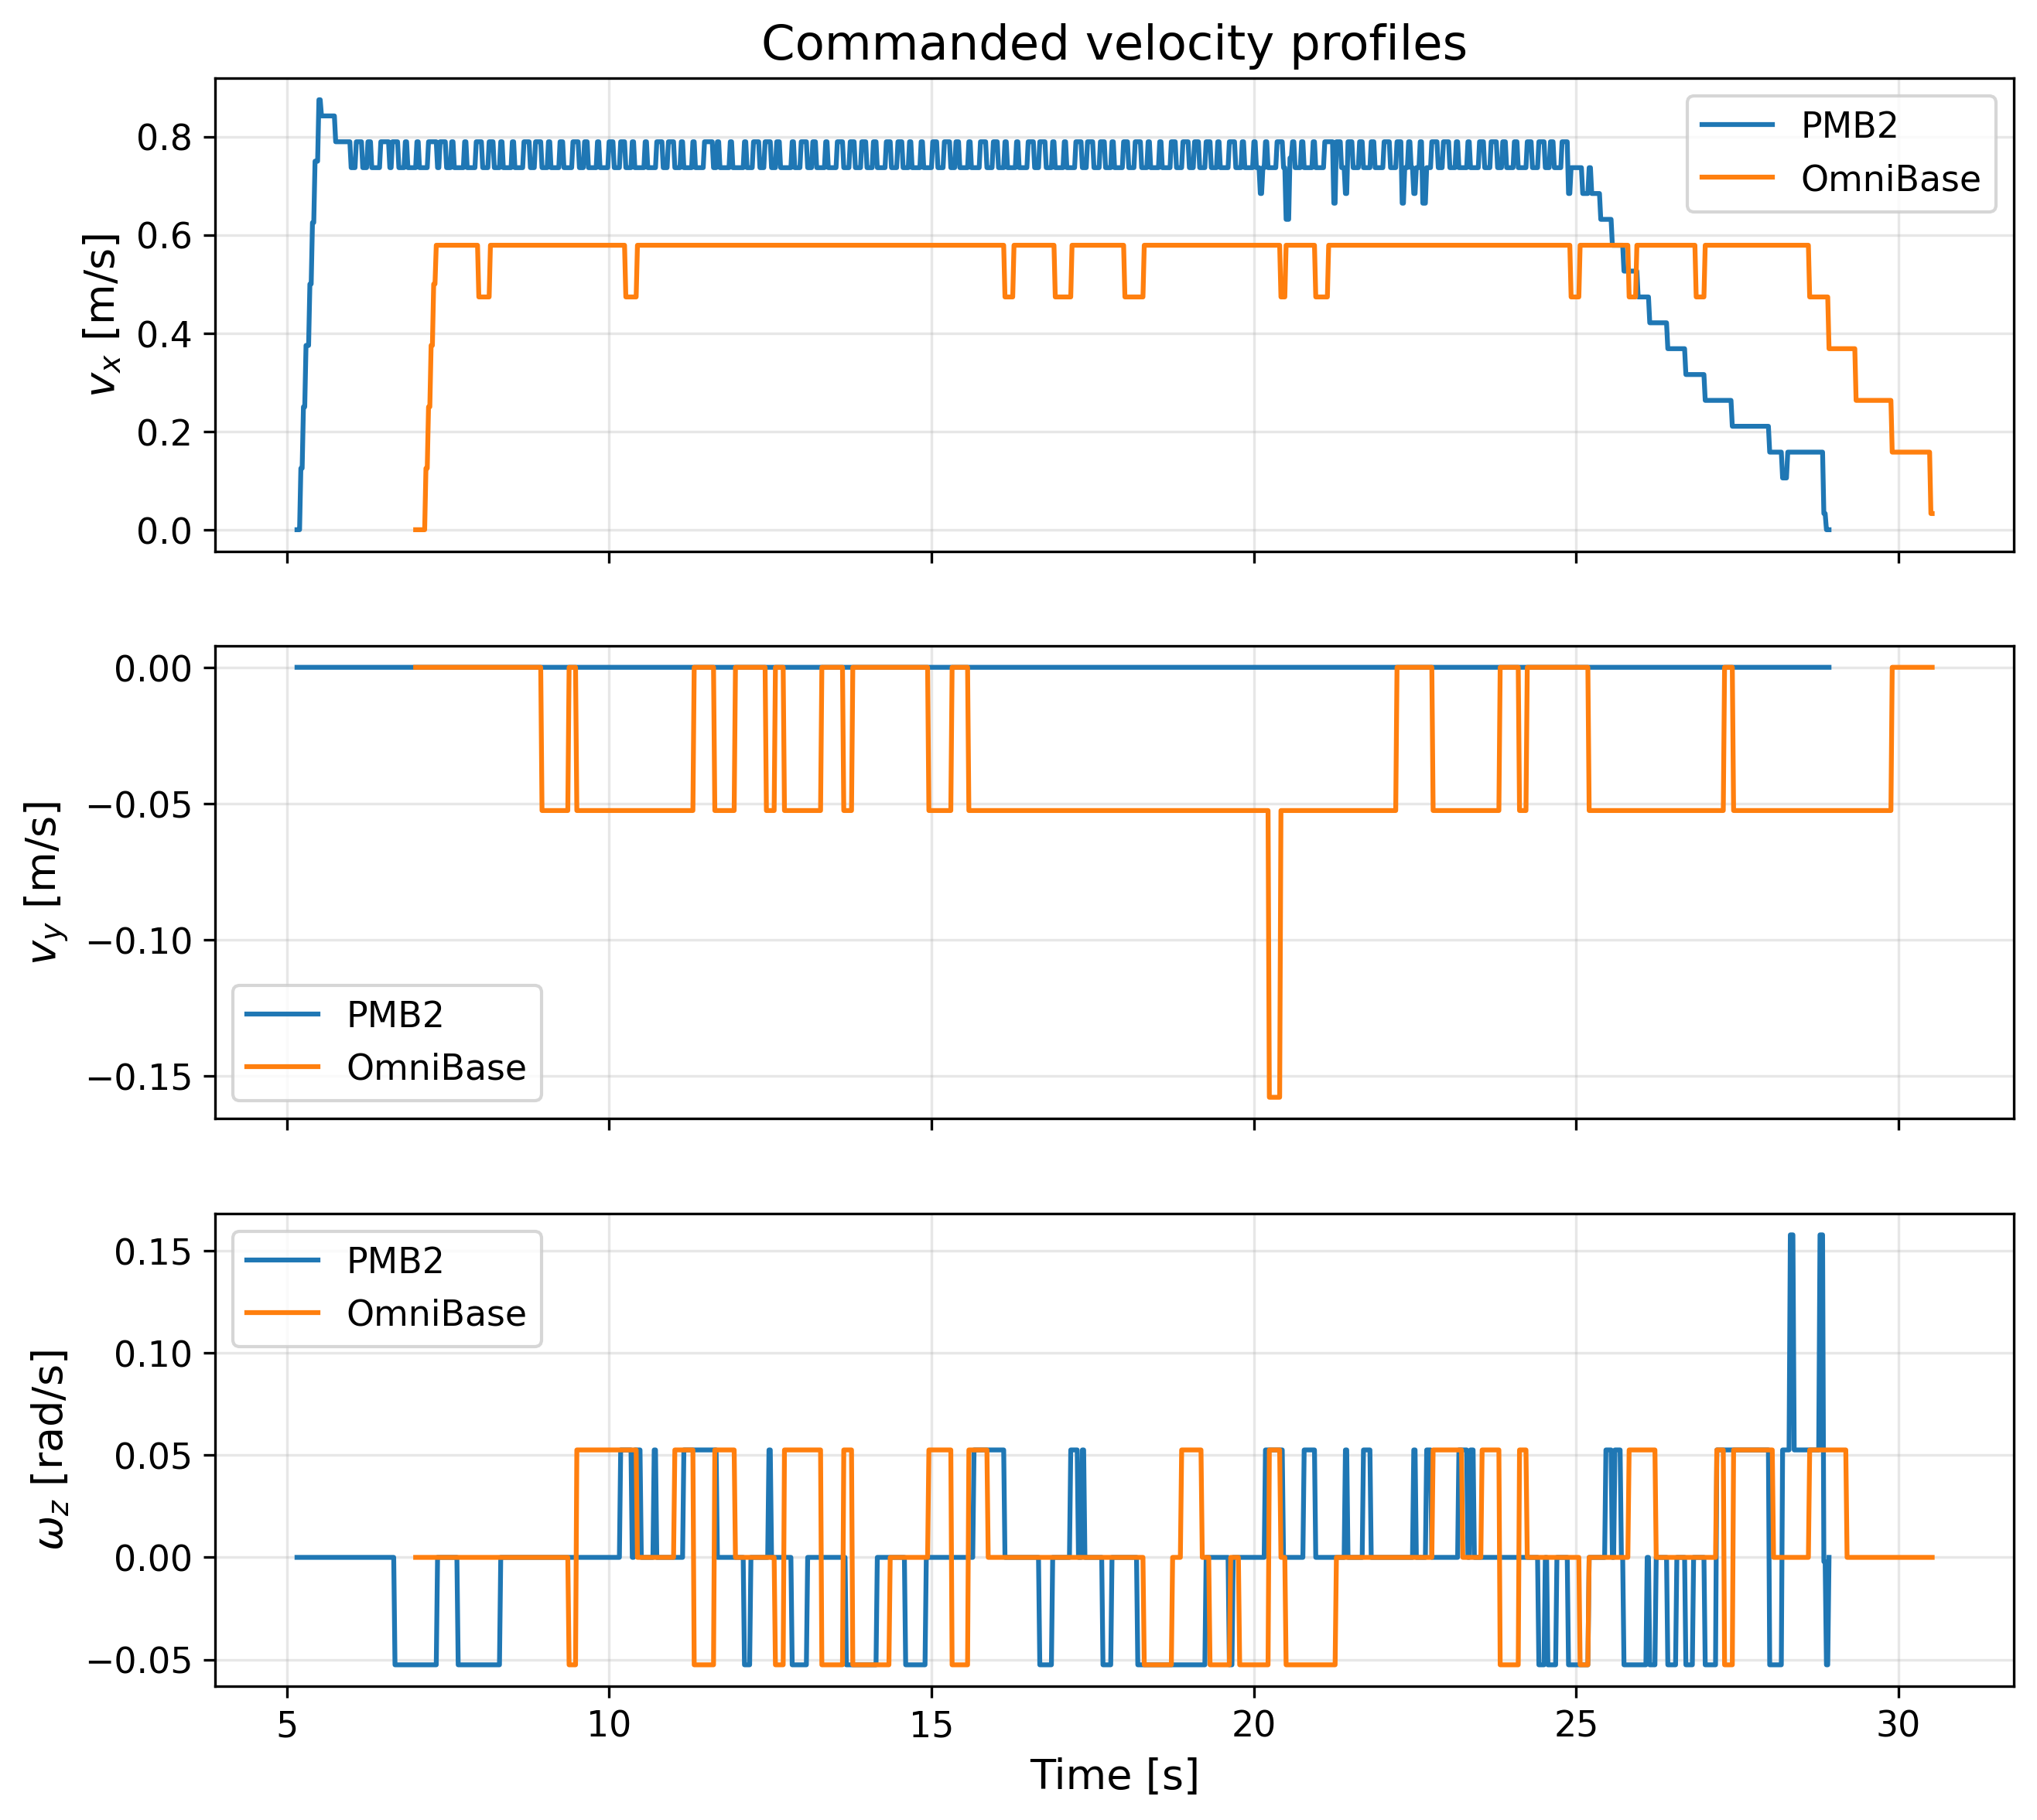
\includegraphics[width=1\textwidth]{images/Ch4/hallway/velocity_profiles.png}
  \caption{Straight corridor: commanded velocity profiles for the median run of each base. The OmniBase uses lateral velocity $v_y$ (centre) to correct drift, whereas the differential PMB2 keeps $v_y \equiv 0$ and relies on $\omega_z$ (bottom).}
  \label{fig:hallway-vel}
\end{figure}

The wheel-rotation profiles of Figures~\ref{fig:hallway-wheels-pmb2} and~\ref{fig:hallway-wheels-omni} complete the kinematic picture and connect these results to the models of Chapter~\ref{Ch:Kinematic}. For the differential PMB2, the left and right traction wheels rotate almost in unison and their position grows monotonically, the expected signature of straight-line motion with negligible steering; the accompanying velocity trace is obtained by differentiating the joint position, because the simulator returns an unreliable wheel-velocity field for this base. For the OmniBase, the four mecanum wheels cannot be read meaningfully from the simulator, since the \texttt{gazebo\_ros\_planar\_move} plugin imposes the body twist directly rather than actuating the wheels; the curves shown are therefore reconstructed by applying the inverse kinematic model of Chapter~\ref{Ch:Kinematic} to the commanded velocities, and depict the ideal, no-slip rotation that would realise the observed motion. They are included as an illustration of the wheel-level behaviour predicted by the kinematics, not as a measured signal.

\begin{figure}[htpb]
  \centering
  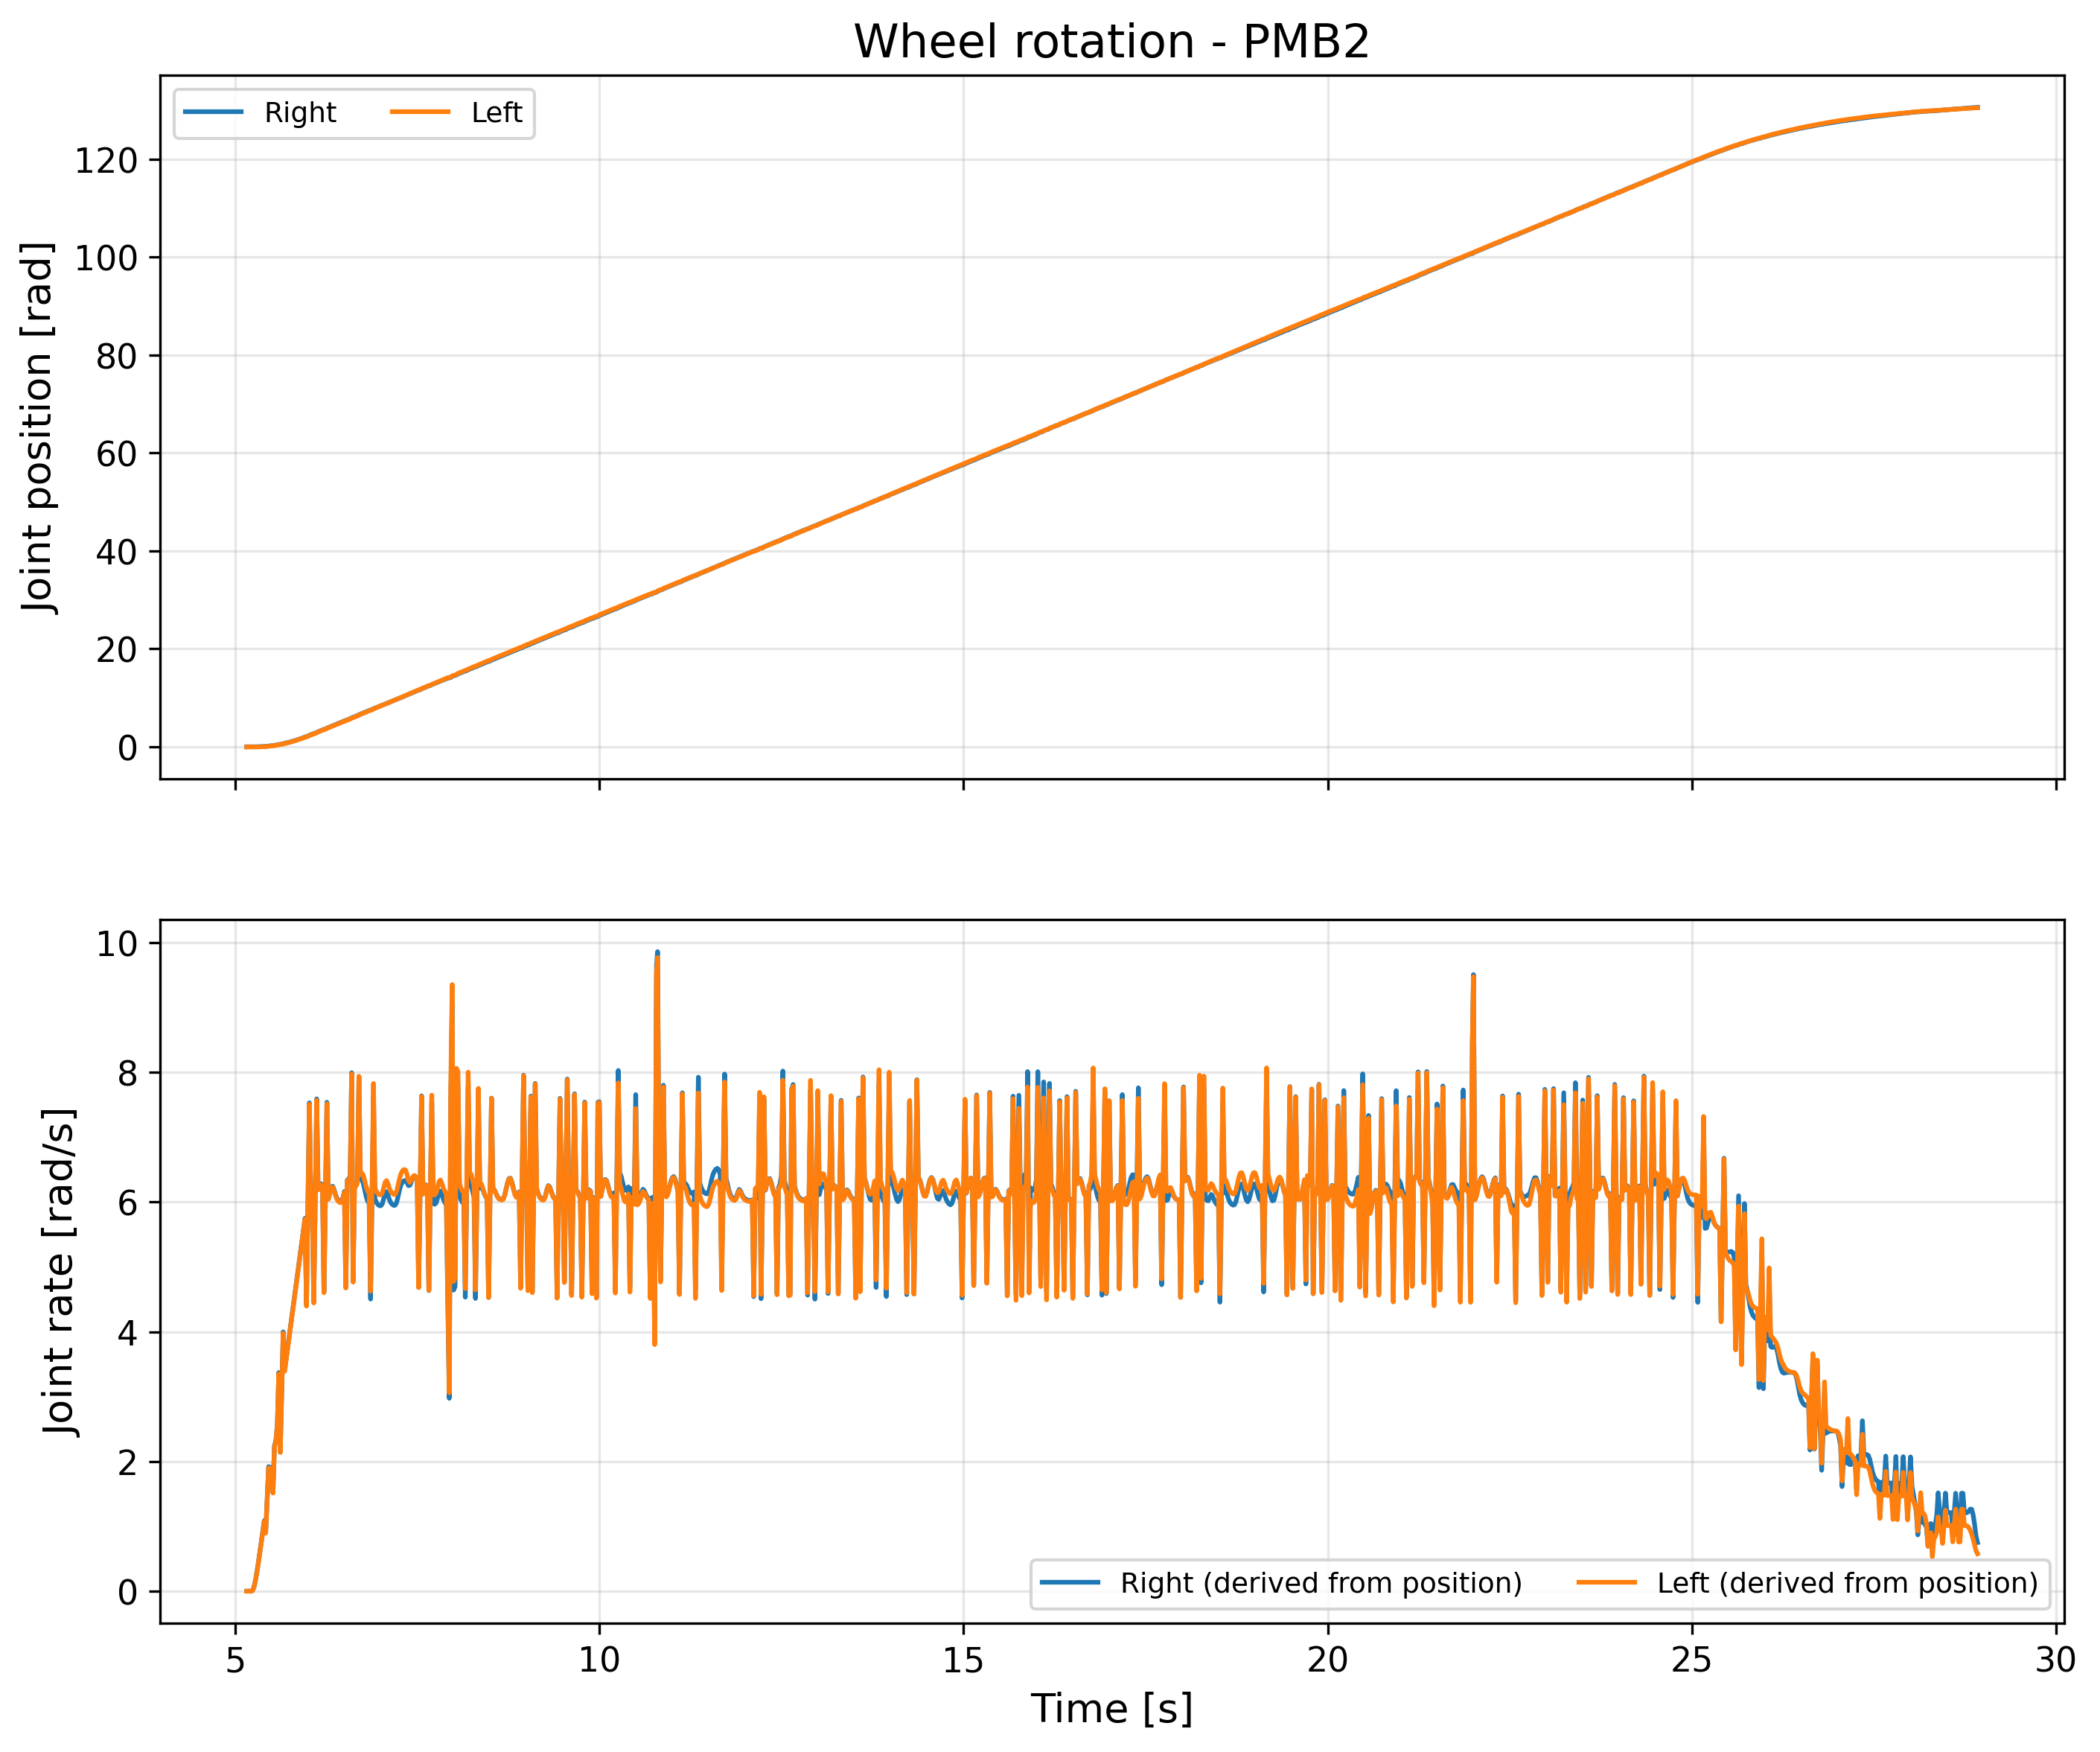
\includegraphics[width=1\textwidth]{images/Ch4/hallway/wheel_rotation_pmb2.png}
  \caption{Straight corridor: wheel rotation over time for the differential PMB2. The two traction wheels rotate almost identically, consistent with straight-line motion. The joint velocity (lower sub-panel) is derived numerically from the joint position, since the \texttt{velocity} field is unreliable in simulation; the resulting rotation is an ideal, no-slip one, which on a flat floor is effectively equivalent to the wheels' measured behaviour.}
  \label{fig:hallway-wheels-pmb2}
\end{figure}

\begin{figure}[htpb]
  \centering
  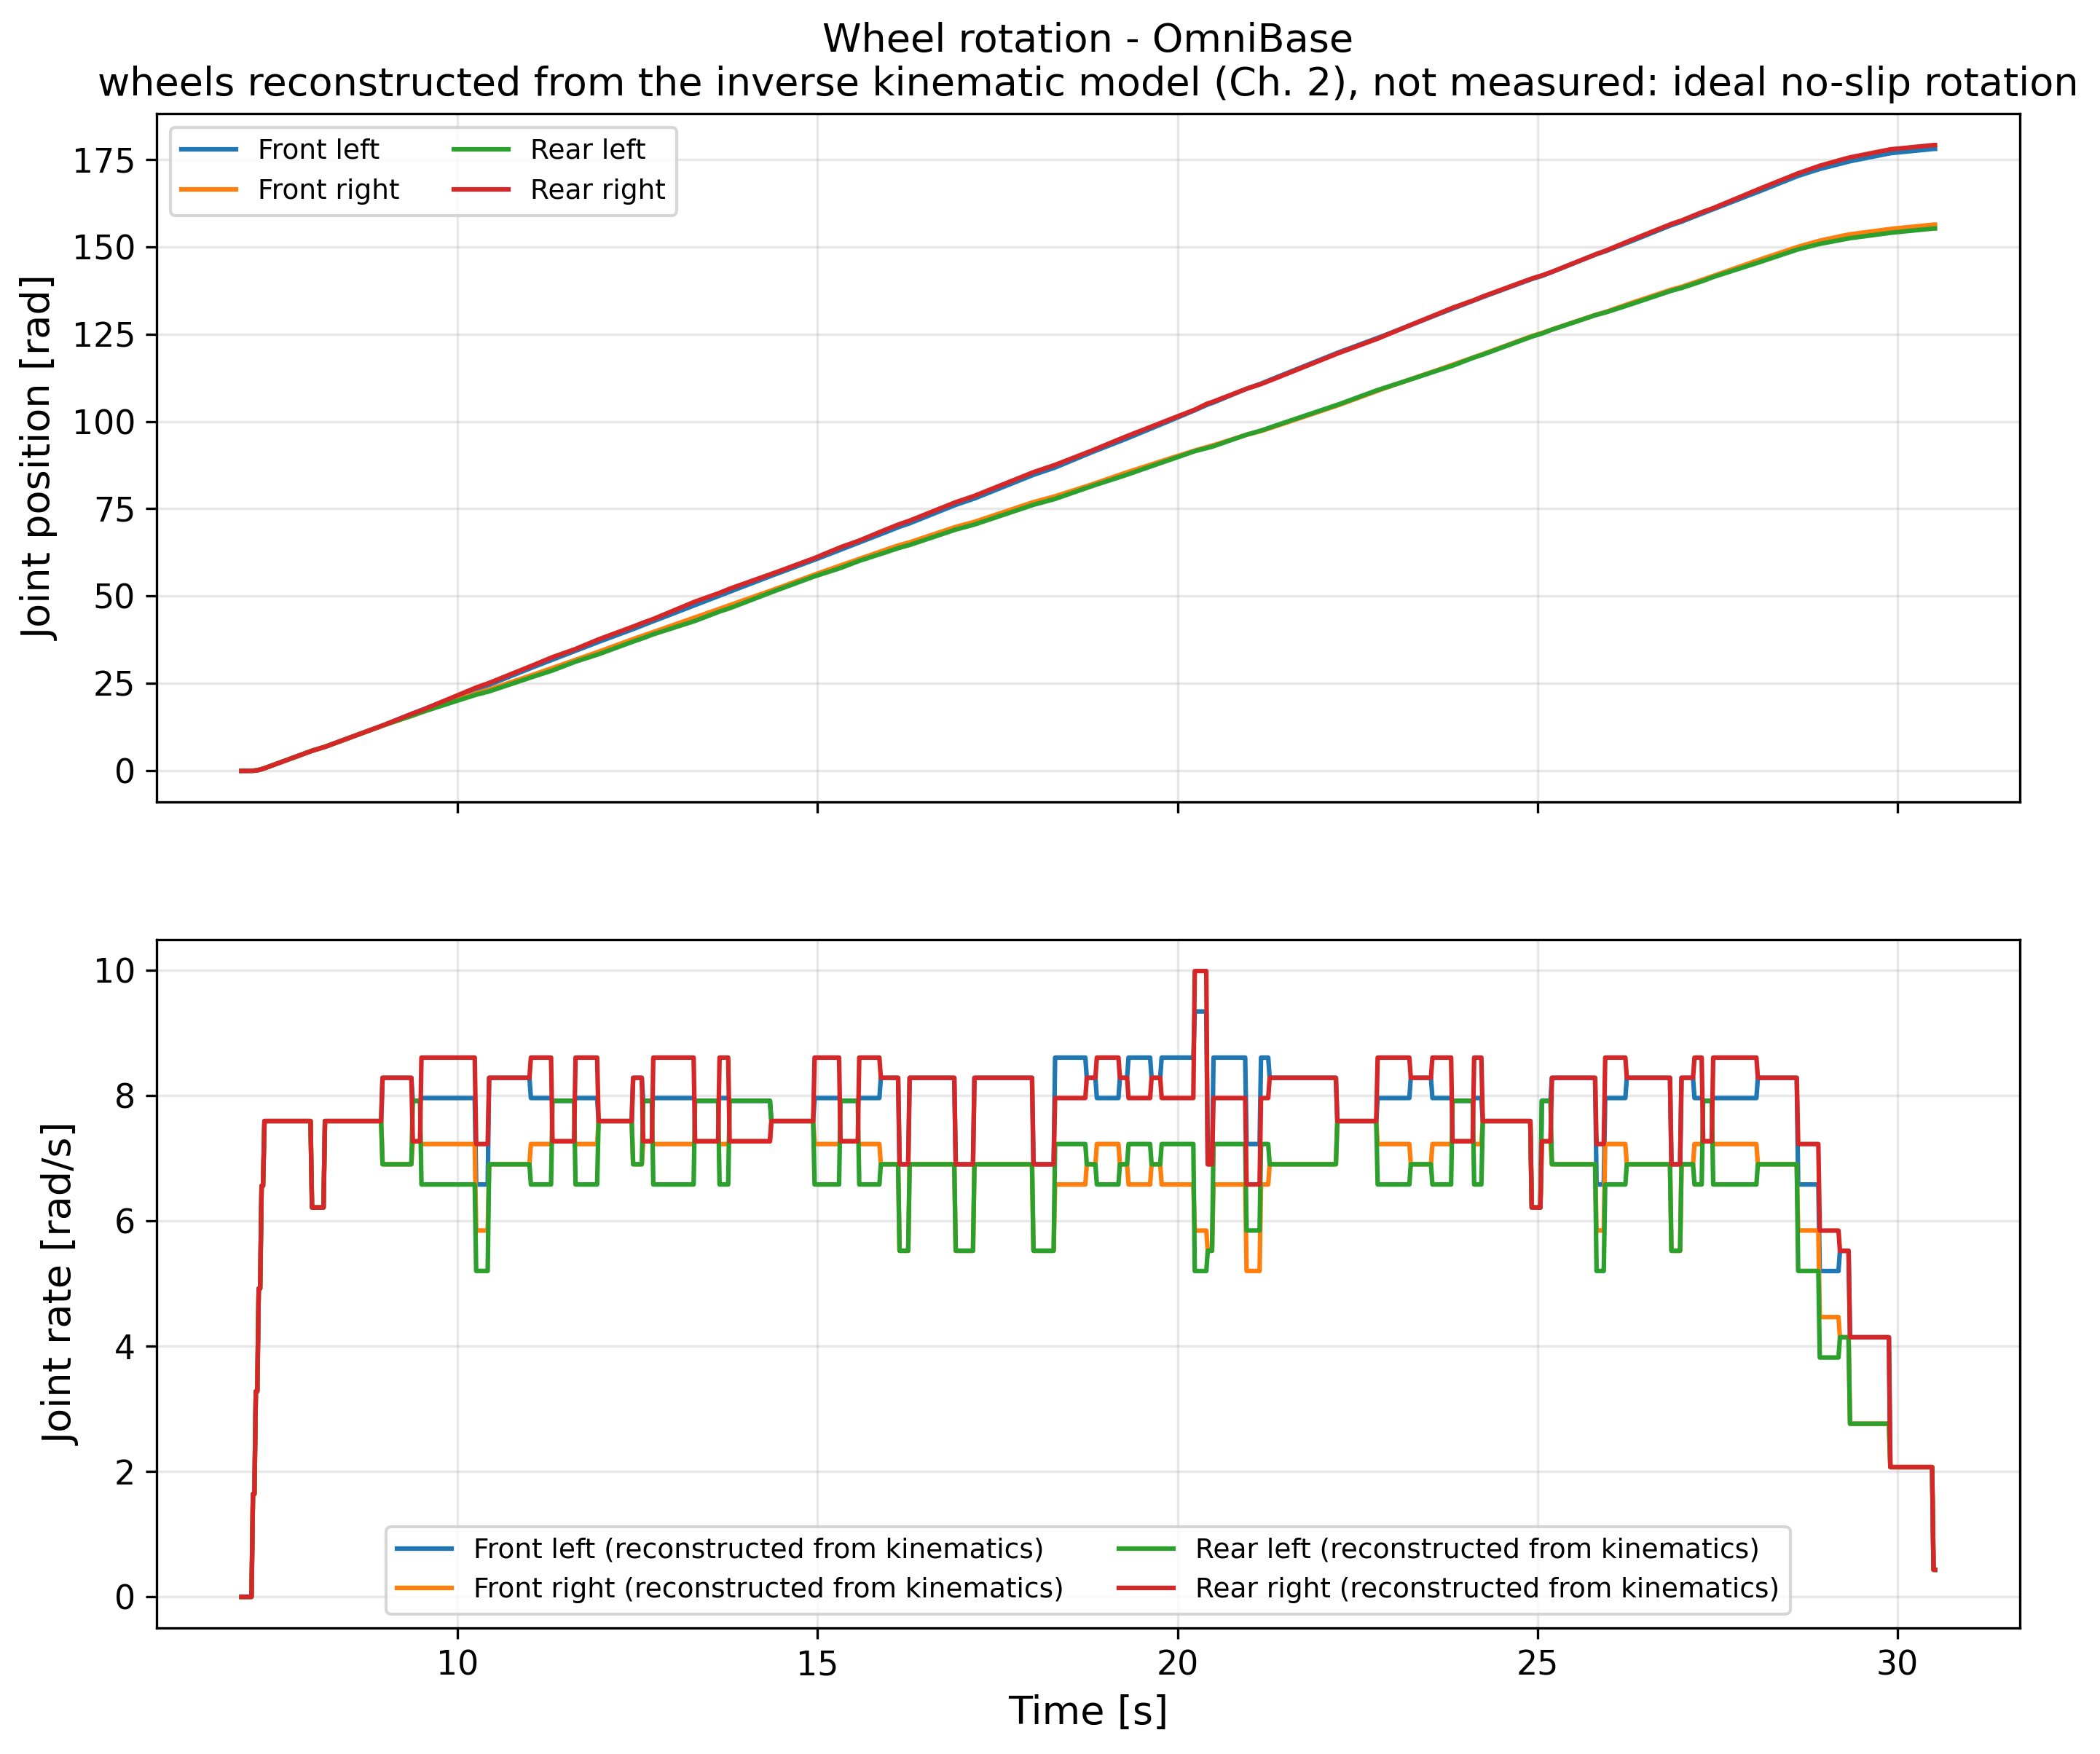
\includegraphics[width=1\textwidth]{images/Ch4/hallway/wheel_rotation_omni.png}
  \caption{Straight corridor: wheel rotation over time for the holonomic OmniBase. The four mecanum wheels are not read from the simulator---the \texttt{gazebo\_ros\_planar\_move} plugin imposes the body twist directly---but reconstructed by applying the inverse kinematic model of Chapter~\ref{Ch:Kinematic} to the commanded velocities, and therefore represent an ideal, no-slip rotation rather than a measured quantity. This shares the same idealised regime as the PMB2 wheel rotation of Figure~\ref{fig:hallway-wheels-pmb2}, which makes the two comparable at the kinematic level while remaining distinct from a comparison of actuation fidelity.}
  \label{fig:hallway-wheels-omni}
\end{figure}




At the goal the two platforms are comparably accurate, with a Ground~Truth positioning error of $0.238$~m for the OmniBase against $0.269$~m for the PMB2---both close to the $0.25$~m goal tolerance, the small excess reflecting the residual localisation offset at the stopping point. The OmniBase additionally shows a minor ($\approx 0.08$~m) offset already at the start waypoint, absent for the differential and attributable to a small initial-placement discrepancy, well within tolerance and without effect on task completion. In terms of efficiency the two bases are close, the OmniBase being marginally faster and markedly more repeatable ($23.56 \pm 0.14$~s against $24.10 \pm 0.52$~s), although part of this lower variance is itself a consequence of its idealised actuation (Section~\ref{subsec:m-fidelity}). Overall, on this trivial route holonomy translates into modestly tighter and smoother tracking, while the differential base remains fully competitive; the substantive differences between the two kinematics emerge only in the more demanding scenarios that follow.


\subsection{Sharp 90-Degree Corner (Path~B)}
\label{subsec:res-angle}

The sharp corner reverses the ranking observed on the straight corridor. Here the holonomic OmniBase is dramatically faster---it completes the route in $4.40 \pm 0.44$~s against $12.86 \pm 0.56$~s for the differential PMB2, almost a threefold difference---yet it tracks the planned path markedly \emph{worse}, its mean deviation from the Nav2 plan being about four times larger ($0.233$ against $0.055$~m). Both platforms again reached the goal in every run without planning failures; the only recovery recorded across the two simple routes was a single costmap-clearing action in one PMB2 run. The aggregate metrics are reported in Table~\ref{tab:angle}, and the two navigation strategies are contrasted in Figure~\ref{fig:angle-traj}.

\begin{table}[htbp]
\centering
\caption{Sharp corner (Path~B): aggregate metrics, mean $\pm$ standard deviation over five runs.}
\label{tab:angle}
\begin{tabular}{lcc}
\toprule
Metric & PMB2 (differential) & OmniBase (holonomic) \\
\midrule
Completion time [s]              & $12.86 \pm 0.56$ & $4.40 \pm 0.44$ \\
Average speed [m/s]              & $0.155 \pm 0.006$ & $0.429 \pm 0.040$ \\
Tracking error, mean [m]        & $0.055 \pm 0.012$ & $0.233 \pm 0.011$ \\
Tracking error, RMS [m]         & $0.104 \pm 0.004$ & $0.287 \pm 0.009$ \\
Mean waypoint error [m]         & $0.230 \pm 0.004$ & $0.316 \pm 0.016$ \\
Corner (WP1) waypoint error [m] & $0.590 \pm 0.004$ & $0.776 \pm 0.019$ \\
Mean orientation error [rad]    & $0.661 \pm 0.014$ & $0.048 \pm 0.022$ \\
Linear smoothness [m/s$^2$]     & $1.174 \pm 0.099$ & $1.827 \pm 0.117$ \\
Angular smoothness [rad/s$^2$]  & $1.849 \pm 0.191$ & $1.014 \pm 0.127$ \\
Lateral usage                    & $0.000 \pm 0.000$ & $0.669 \pm 0.016$ \\
\bottomrule
\end{tabular}
\end{table}

\begin{figure}[H]
  \centering
  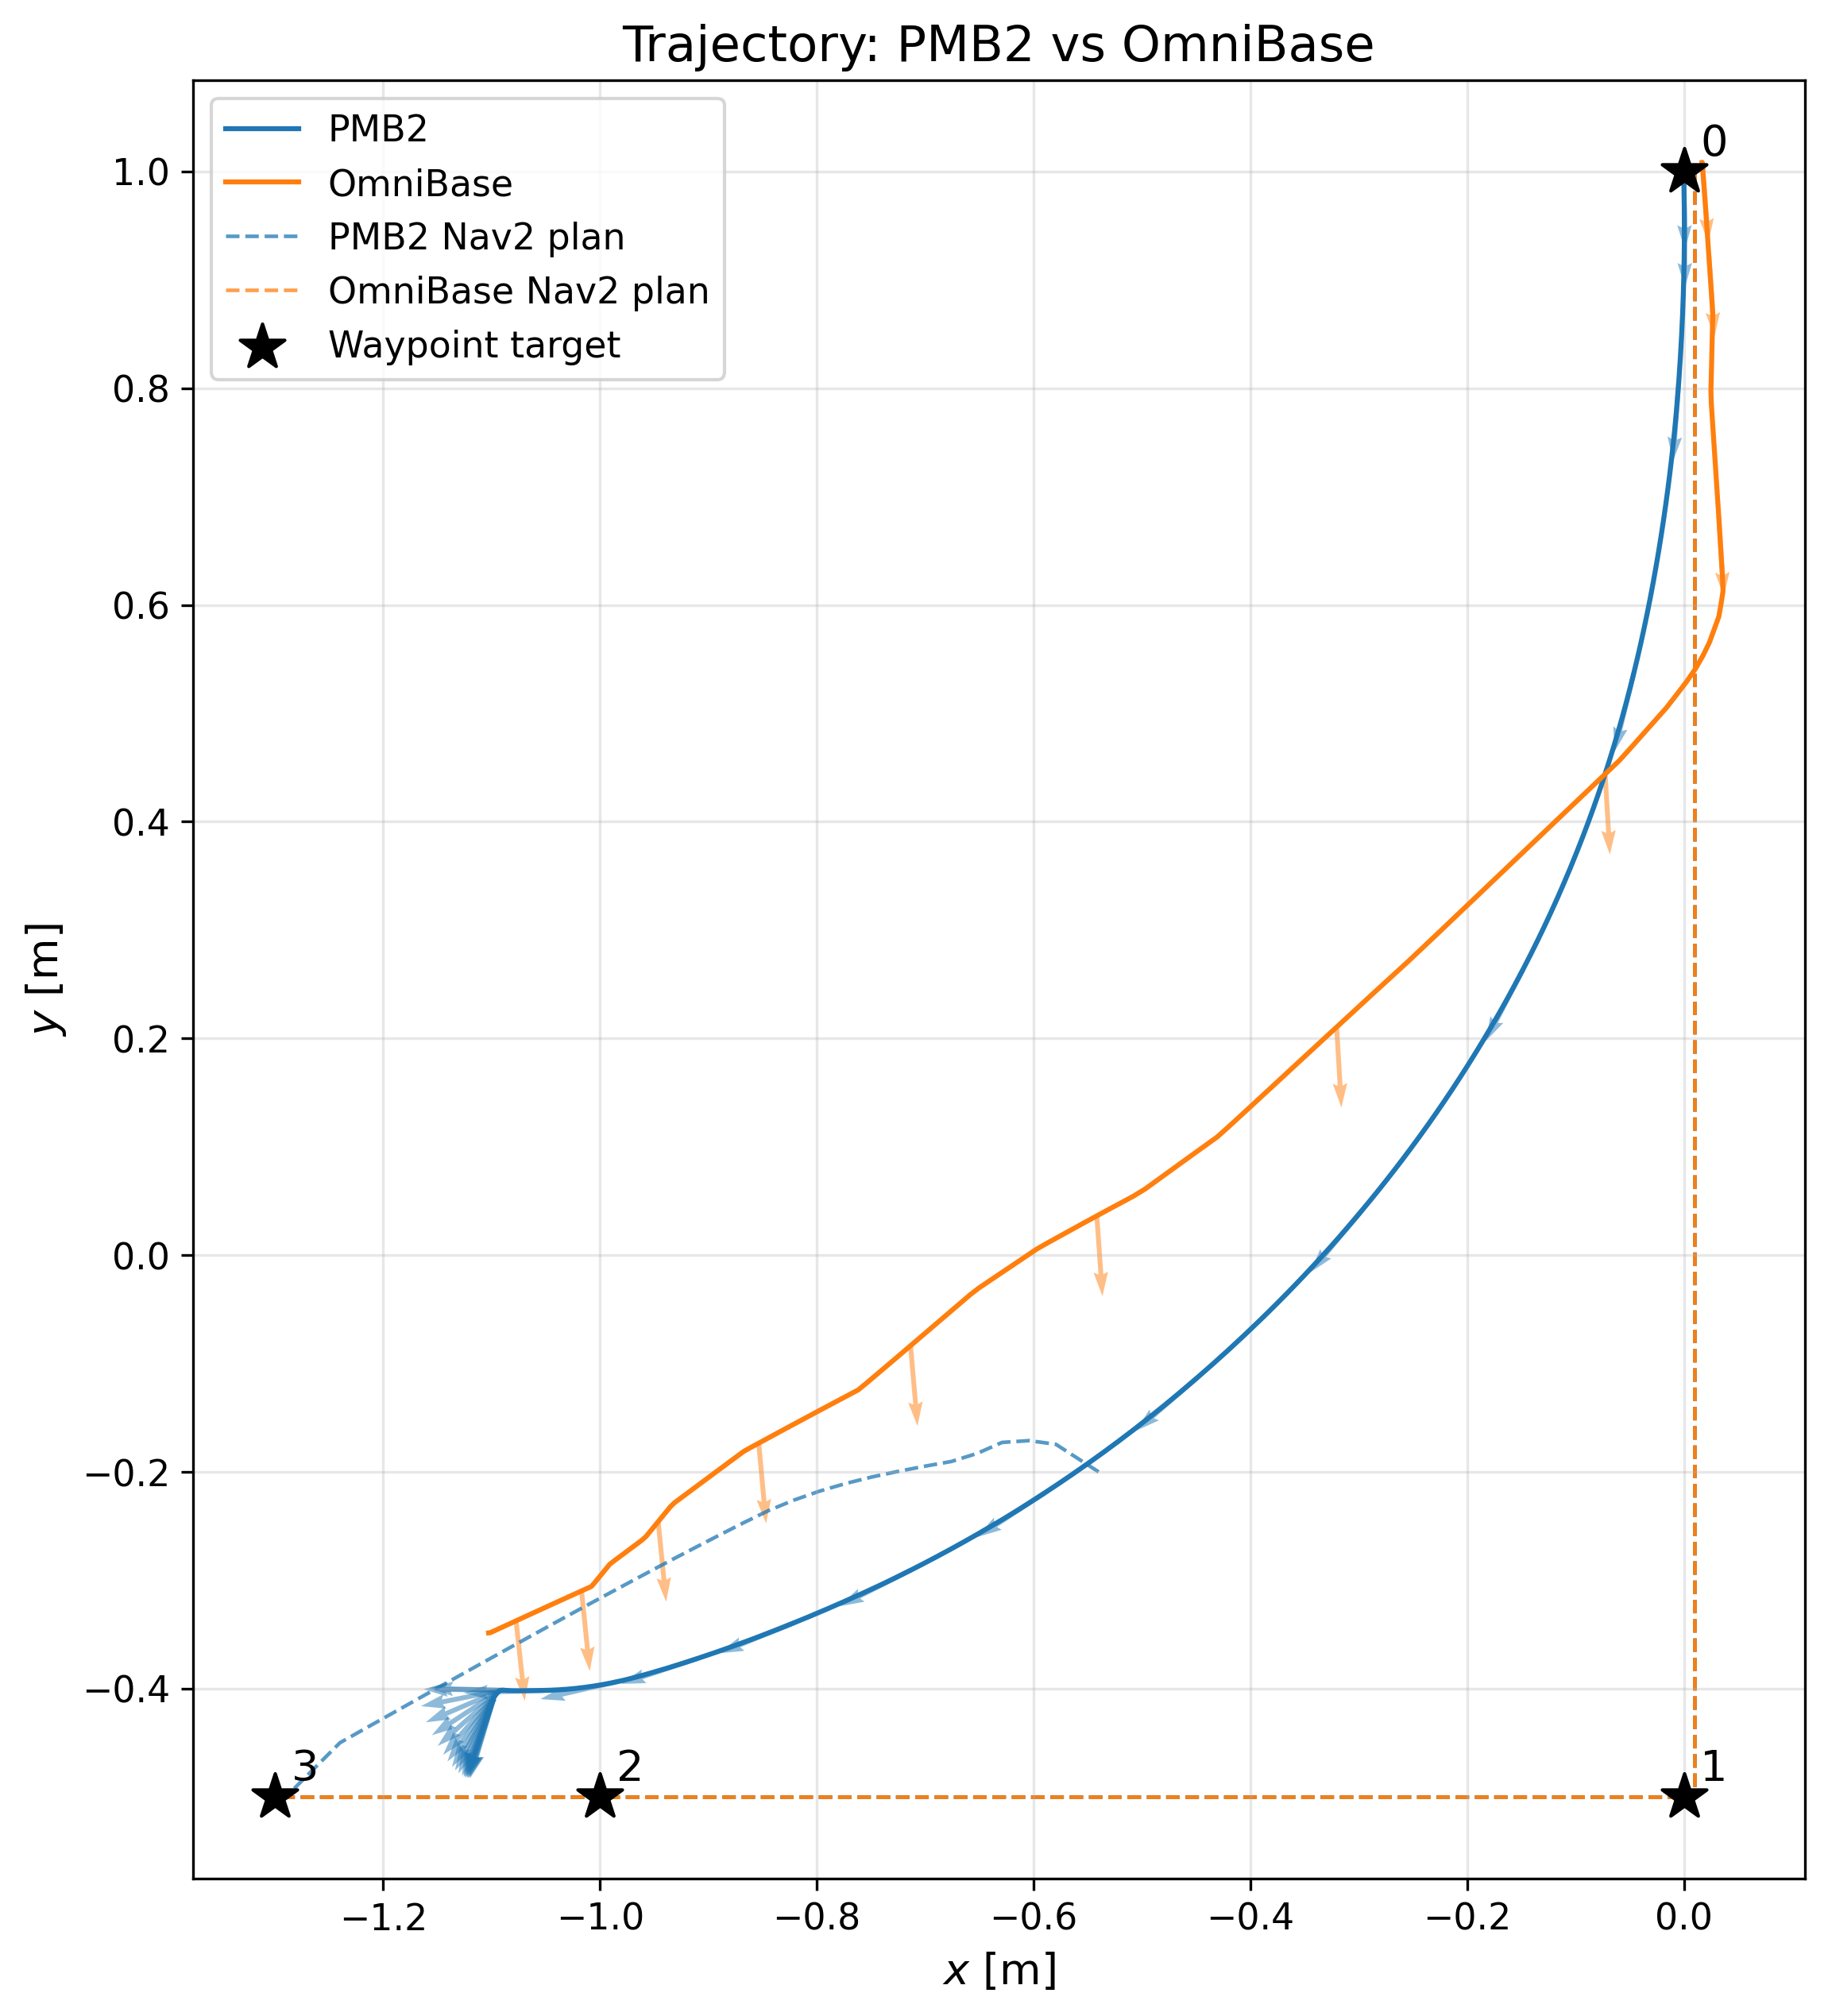
\includegraphics[width=1\textwidth]{images/Ch4/angle/trajectory_comparison.png}
  \caption{Sharp corner: Ground~Truth trajectory of the median run of each base, with the corresponding Nav2 global plans (dashed) and heading arrows. Neither base reaches the corner waypoint (WP1): both round it. The OmniBase keeps a fixed south-facing heading while strafing along a diagonal shortcut, whereas the PMB2 rotates to follow the path tangent and performs a final in-place rotation near the goal.}
  \label{fig:angle-traj}
\end{figure}

Because \texttt{NavigateThroughPoses} does not stop at the intermediate poses, both platforms cut the corner heavily: neither approaches the corner waypoint (WP1) closer than about $0.6$~m (PMB2) or $0.8$~m (OmniBase), and this closest-approach distance---following the definition of Section~\ref{subsec:m-accuracy}---is precisely the extent of the corner-cutting rather than a positioning failure. The manner of the cut, however, differs fundamentally. The OmniBase exploits its lateral degree of freedom (lateral usage $0.669$) to translate diagonally towards the second leg while holding an almost constant heading, tracing a single straight shortcut. The PMB2, unable to strafe, negotiates the turn as a smooth curve, continuously rotating so that its heading follows the direction of travel, as the arrows in Figure~\ref{fig:angle-traj} show.

\begin{figure}[H]
  \centering
  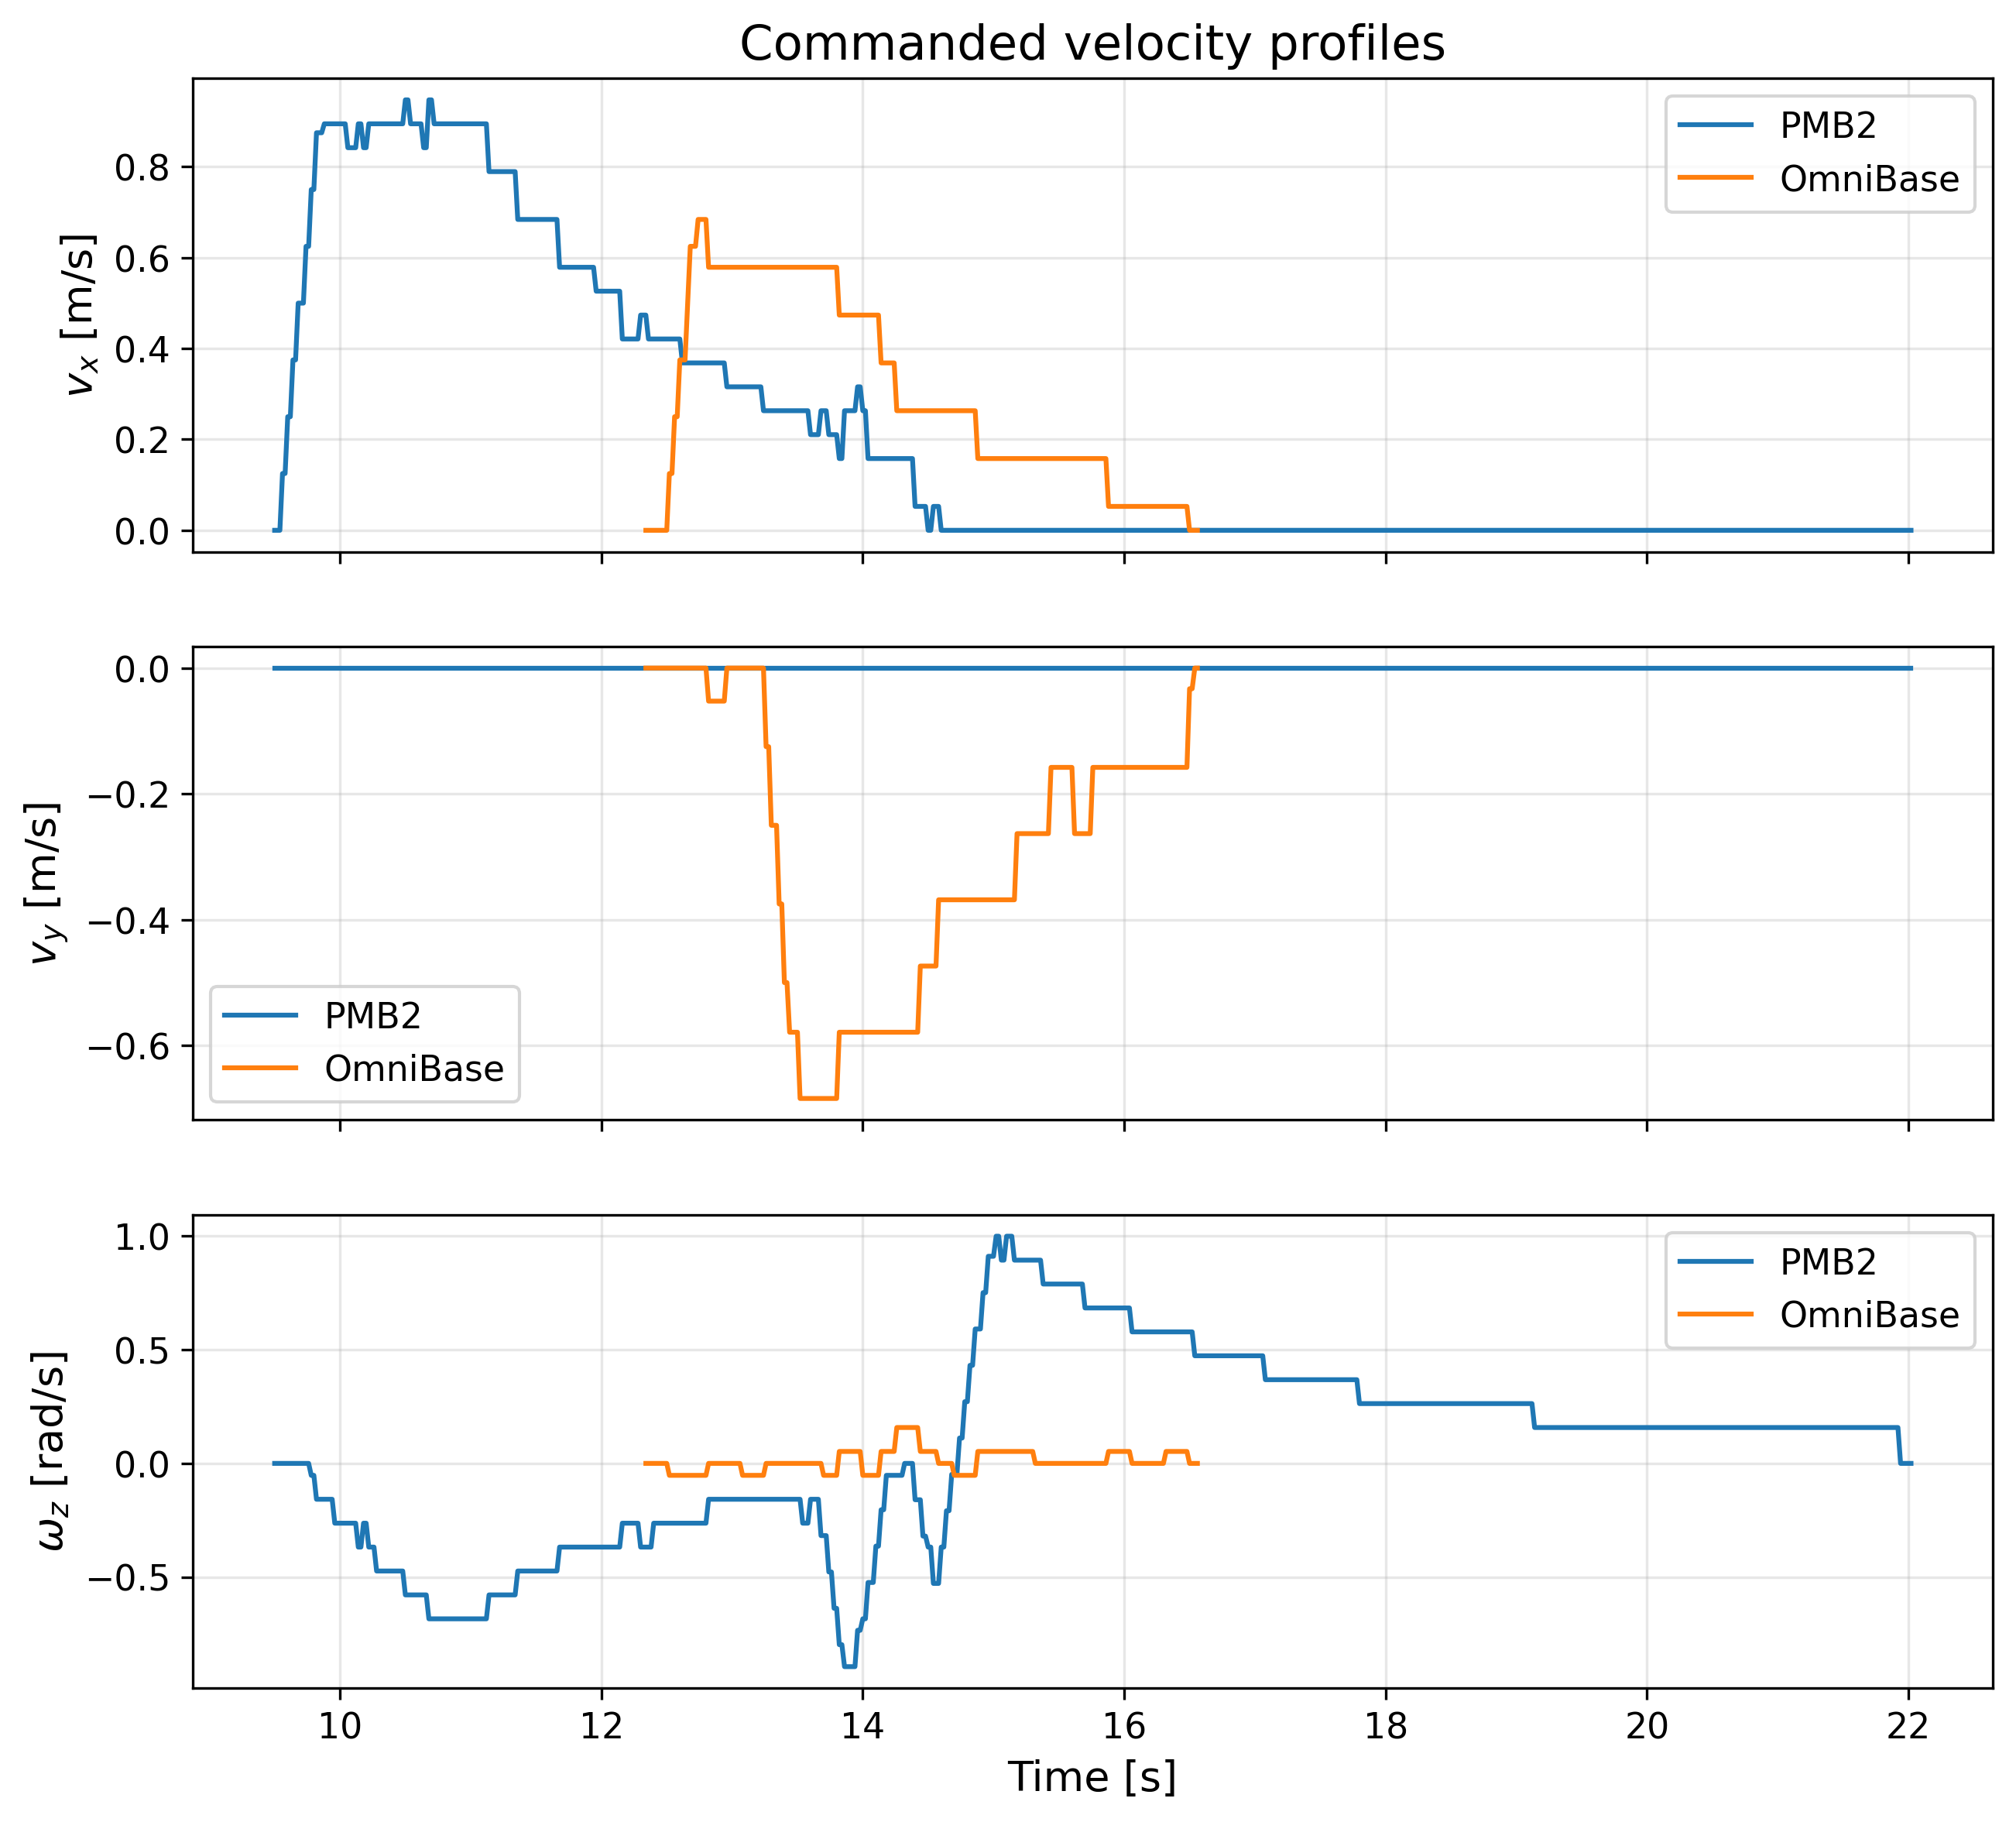
\includegraphics[width=1\textwidth]{images/Ch4/angle/velocity_profiles.png}
  \caption{Sharp corner: commanded velocity profiles for the median run of each base. The OmniBase performs the turn through a pulse of lateral velocity $v_y$ (centre) with $\omega_z \approx 0$, while the PMB2 keeps $v_y \equiv 0$ and turns through $\omega_z$, including a pronounced terminal burst (bottom) corresponding to the final in-place rotation.}
  \label{fig:angle-vel}
\end{figure}

The velocity profiles of Figure~\ref{fig:angle-vel} make the two mechanisms explicit and explain the large time gap. The OmniBase realises the entire manoeuvre with a single burst of lateral velocity (peaking near $-0.7$~m/s) while keeping $\omega_z$ close to zero; it never rotates, and finishes quickly. The PMB2 instead turns entirely through $\omega_z$, and---crucially---arrives at the goal travelling westwards while the commanded final orientation points south, so it must perform a final in-place rotation to satisfy the goal-orientation tolerance. This terminal rotation, visible as the pronounced $\omega_z$ burst and the long low-speed tail at the end of the differential's profile, accounts for a large part of the threefold difference in completion time and for the differential's higher angular acceleration ($1.849$ against $1.014$~rad/s$^2$). The trade-off is mirrored in the linear smoothness, where the ordering is now the opposite of the corridor: the OmniBase is linearly \emph{rougher} ($1.827$ against $1.174$~m/s$^2$), the transient of its sharp strafe outweighing the differential's gentler forward profile.

\begin{figure}[H]
  \centering
  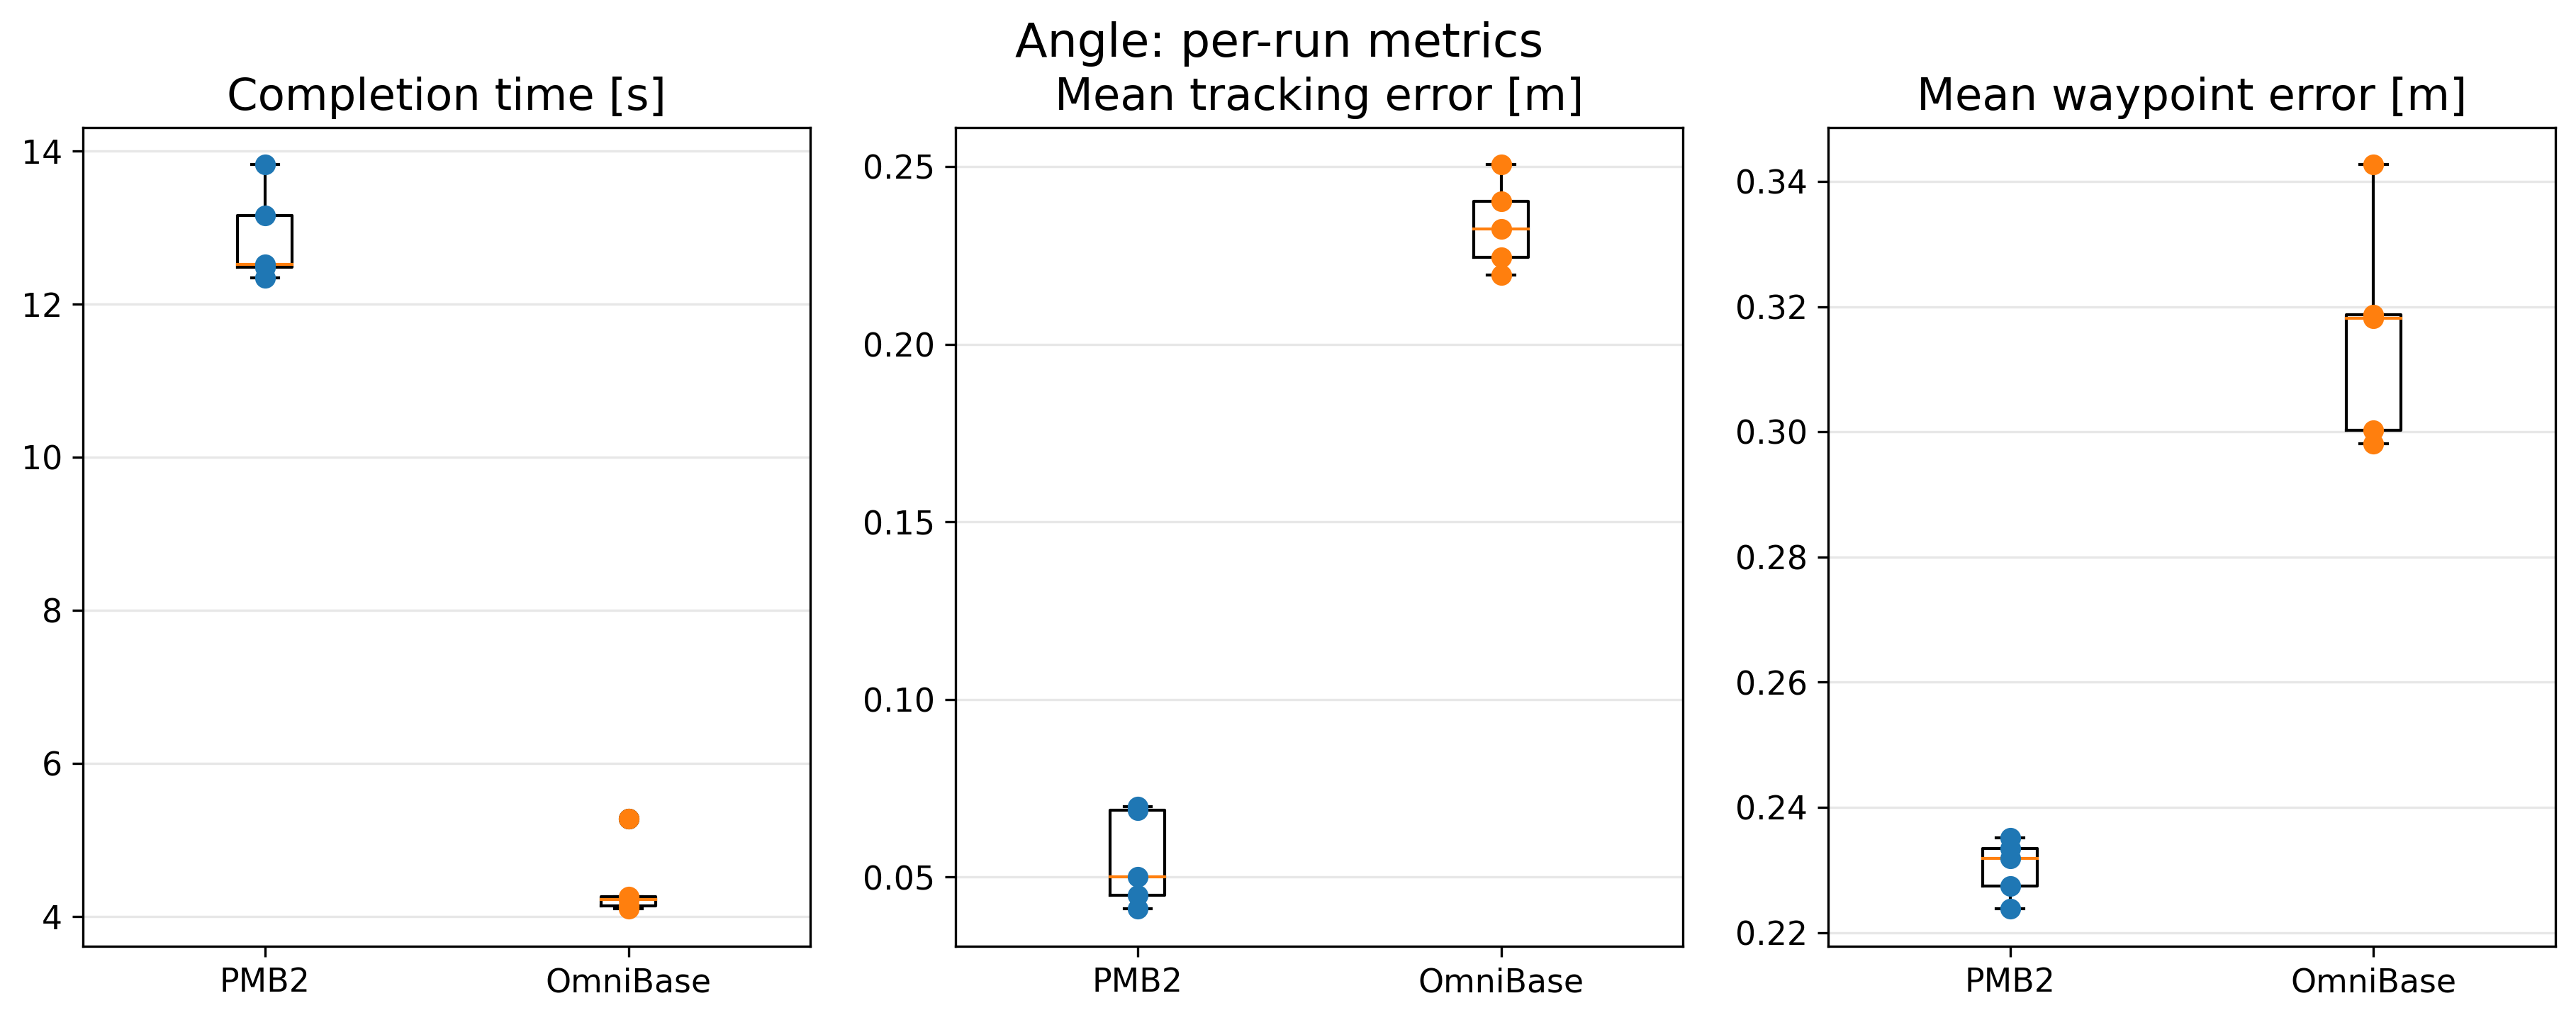
\includegraphics[width=1\textwidth]{images/Ch4/angle/boxplots_Angle.png}
  \caption{Sharp corner: per-run distribution of completion time, mean tracking error, and mean waypoint error. The OmniBase is consistently far faster but exhibits systematically larger tracking and waypoint errors.}
  \label{fig:angle-box}
\end{figure}

The per-run distributions in Figure~\ref{fig:angle-box} confirm that these differences are systematic across repetitions rather than isolated to a single run. The tracking-error reversal deserves emphasis: whereas on the straight corridor holonomy produced tighter path-following, on the corner it is the differential that adheres more closely to the plan. The reason is that the holonomic shortcut, being a single diagonal, departs from the L-shaped global plan over a longer stretch, while the differential follows a curve that hugs the plan more closely and, once past the corner, quickly settles back onto the second leg. Finally, the orientation-error figures ($0.661$~rad for the PMB2 against $0.048$~rad for the OmniBase) must be read through the caveat of Section~\ref{subsec:m-accuracy}: the intermediate waypoint headings are decorative and were all specified towards south, coinciding with the heading the OmniBase happens to maintain while strafing, so its small value reflects heading stability rather than active orientation control; the differential's large value likewise reflects its constantly changing heading along the curve, not a failure to reach a commanded pose. In summary, on a sharp corner holonomy converts into a decisive speed advantage through lateral motion, at the cost of looser adherence to the planned path, whereas the differential drive stays closer to the plan but pays for the required rotations in time and angular effort---the absolute smoothness and variance values remaining subject to the actuation-fidelity caveat of Section~\ref{subsec:m-fidelity}.

\subsection{Cluttered Obstacle Course (Path~C)}
\label{subsec:res-obstacles}

The cluttered obstacle course is the route that most directly probes navigation robustness, and it exposes the sharpest qualitative difference of the whole waypoint campaign. Both platforms completed all five runs and traced the full winding circuit through the eleven waypoints. The decisive difference lies not in whether the goal is reached, but in how much the planning stack struggles to reach it: the differential PMB2 incurred at least one planning failure in \emph{every} run (between one and five, about $4\%$ of its planning attempts), whereas the holonomic OmniBase never failed to plan in any run. The aggregate metrics are reported in Table~\ref{tab:obs}.

Figure~\ref{fig:obs-traj} shows the Ground~Truth trajectories of all five runs of each base. Both platforms trace the full winding circuit through the eleven waypoints, and the geometry of the two sets of paths is essentially the same: the kinematic difference does not alter the route taken, only the way it is executed. The two bases differ, however, in run-to-run consistency. The OmniBase trajectories are almost perfectly superimposed along the entire circuit, whereas the PMB2 ones visibly fan out at a few points---most noticeably along the stretches approaching the lower-left and right portions of the loop---where the five repetitions follow slightly different curves. This higher spatial variability of the differential base is not uniform but concentrates in the tighter sections of the route, and it foreshadows the robustness difference quantified below: the same confined passages that spread the differential's repetitions are those where its global planner will be seen to struggle. Part of the OmniBase's tighter overlap is, in addition, a consequence of its idealised actuation (Section~\ref{subsec:m-fidelity}), so the comparison of repeatability should be read together with that caveat.

\begin{table}[htbp]
\centering
\caption{Cluttered obstacle course (Path~C): aggregate metrics, mean $\pm$ standard deviation over five runs.}
\label{tab:obs}
\begin{tabular}{lcc}
\toprule
Metric & PMB2 (differential) & OmniBase (holonomic) \\
\midrule
Completion time [s]            & $75.6 \pm 3.5$ & $86.1 \pm 29.3$ \\
Average speed [m/s]            & $0.359 \pm 0.015$ & $0.335 \pm 0.076$ \\
Tracking error, mean [m]      & $0.136 \pm 0.011$ & $0.068 \pm 0.009$ \\
Tracking error, RMS [m]       & $0.167 \pm 0.010$ & $0.088 \pm 0.008$ \\
Mean waypoint error [m]       & $0.175 \pm 0.011$ & $0.187 \pm 0.006$ \\
Mean orientation error [rad]  & $1.670 \pm 0.059$ & $0.151 \pm 0.023$ \\
Linear smoothness [m/s$^2$]   & $2.027 \pm 0.085$ & $1.914 \pm 0.301$ \\
Angular smoothness [rad/s$^2$] & $2.833 \pm 0.118$ & $1.217 \pm 0.098$ \\
Lateral usage                  & $0.000 \pm 0.000$ & $0.649 \pm 0.068$ \\
Planning failures              & $2.40 \pm 1.74$ & $0.00 \pm 0.00$ \\
Costmap clears                 & $2.60 \pm 1.63$ & $2.20 \pm 2.93$ \\
Spin / BackUp / Wait           & $0$ / $0$ / $0$ & $0.4$ / $0.2$ / $0.4$ \\
\bottomrule
\end{tabular}
\end{table}

\begin{figure}[H]
  \centering
  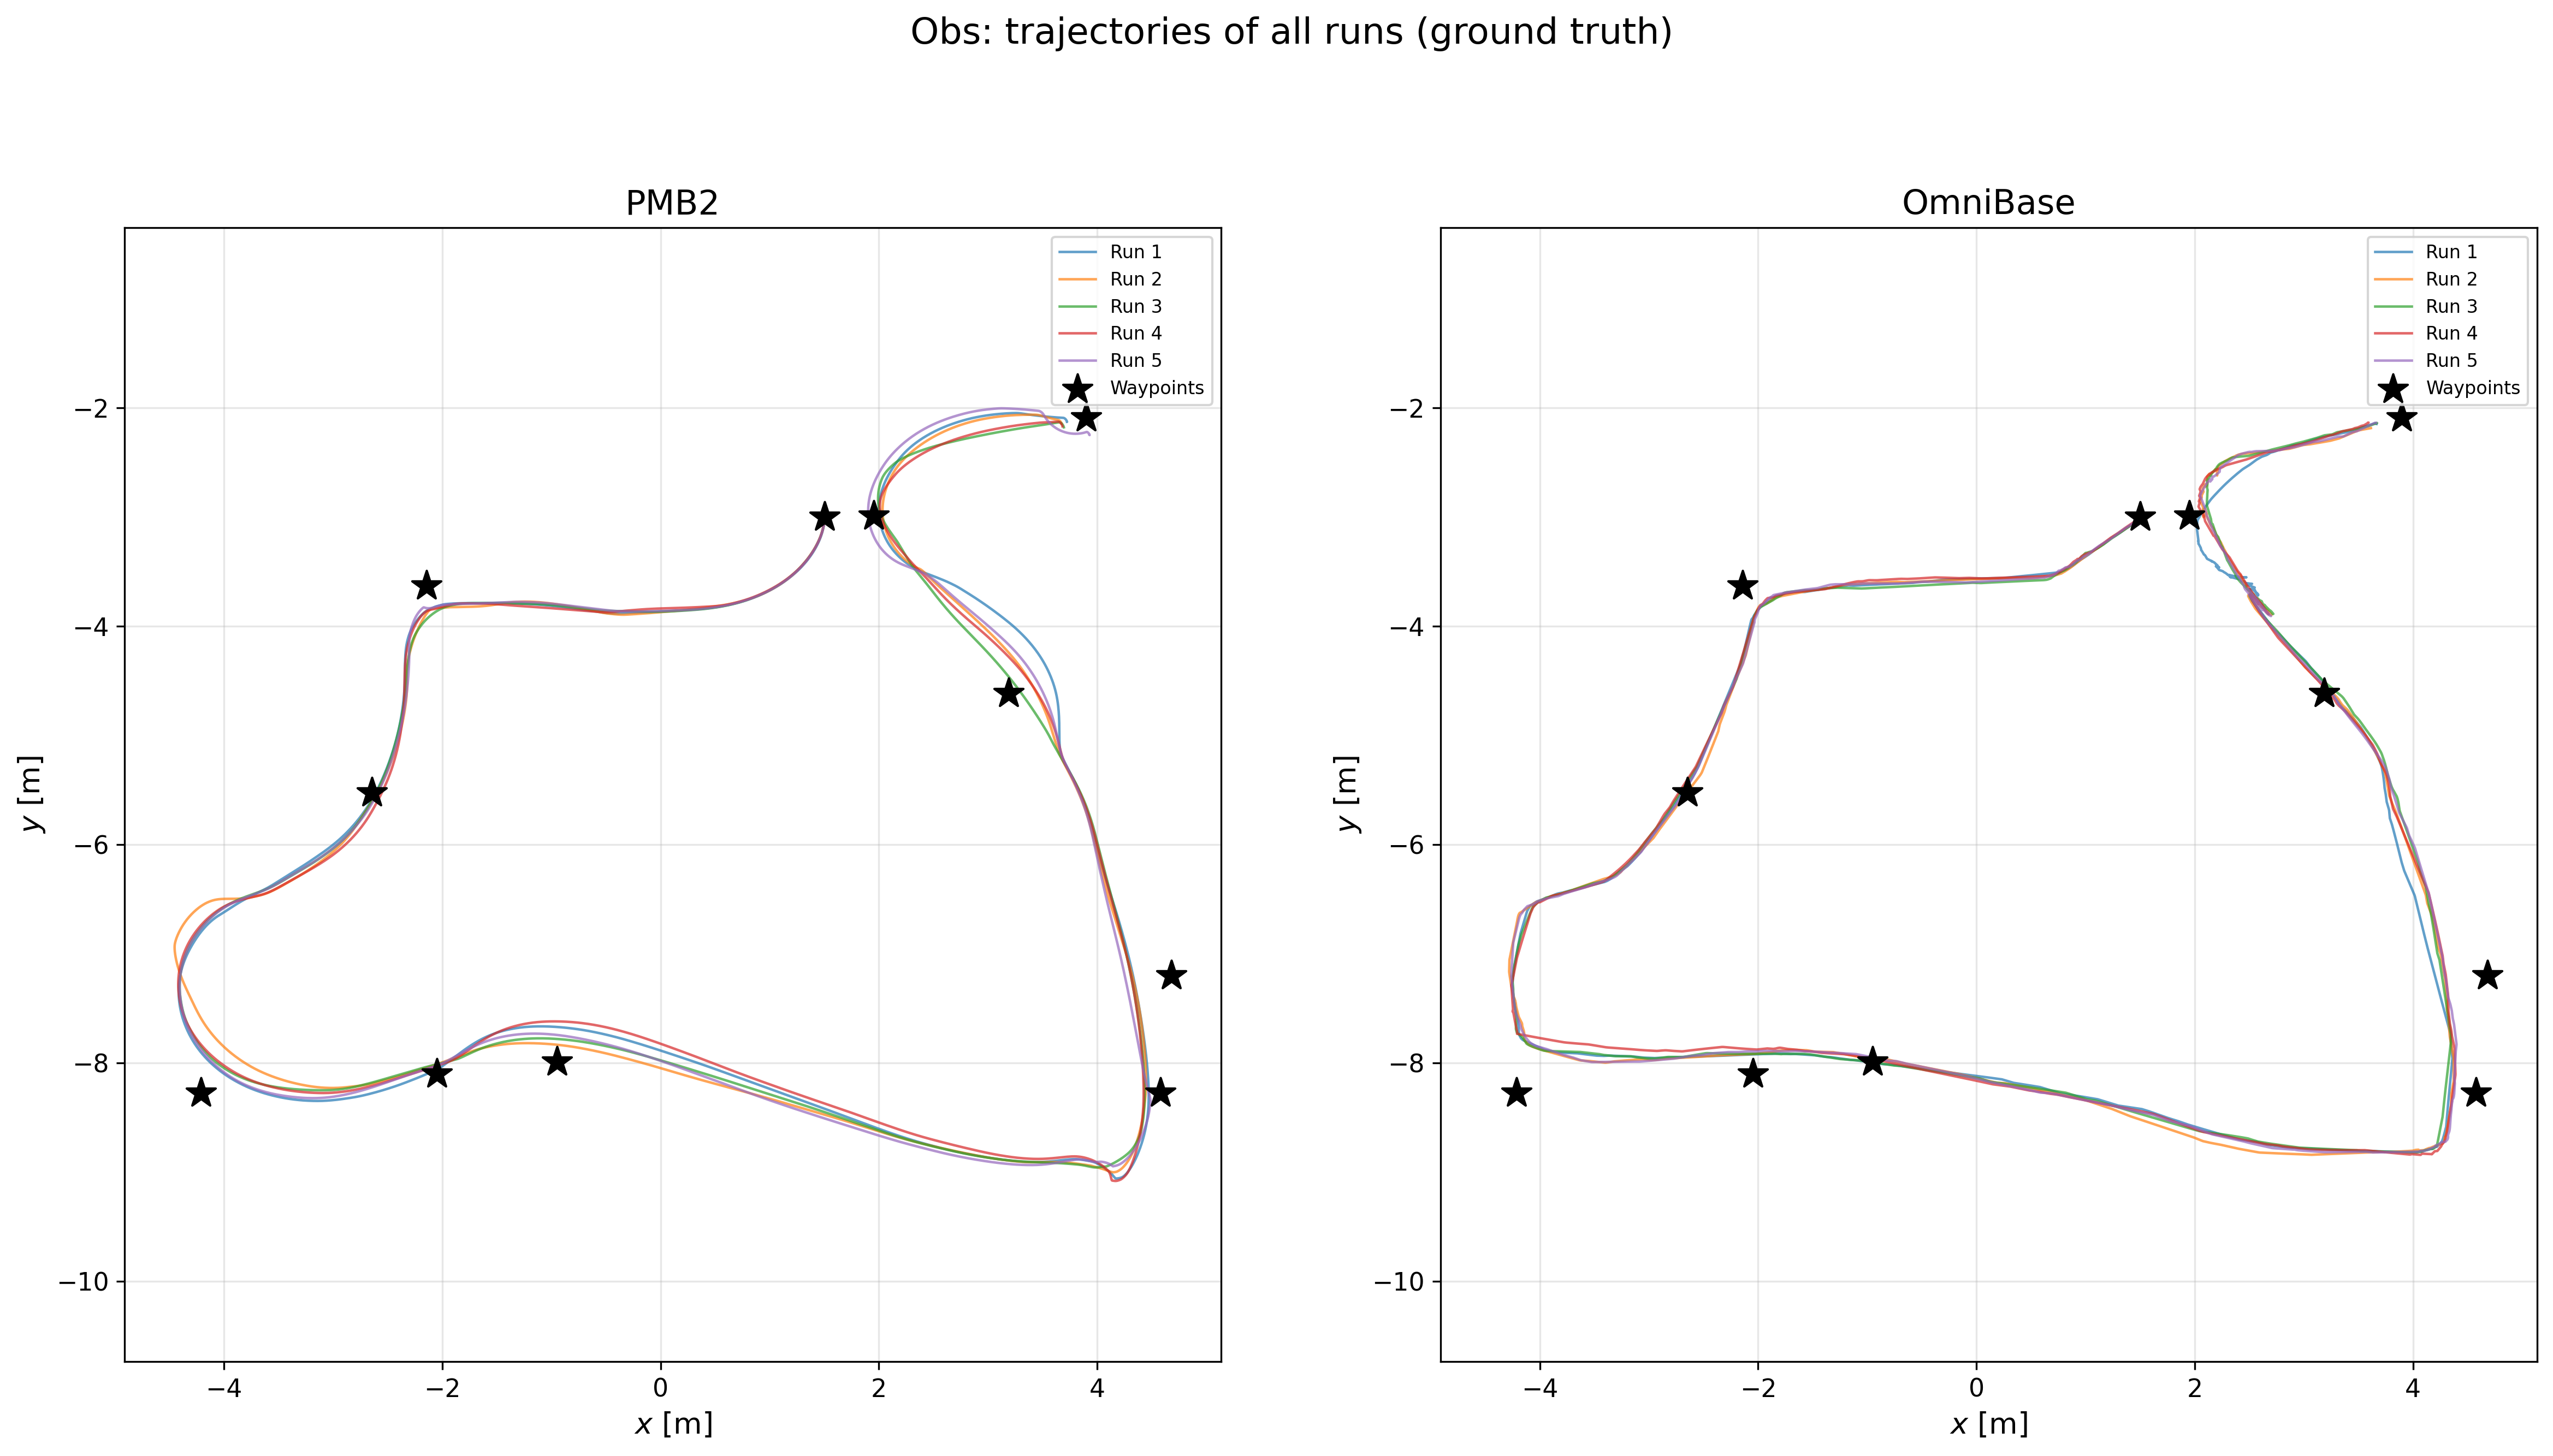
\includegraphics[width=\textwidth]{images/Ch4/obs/trajectories_all_Obs.png}
  \caption{Cluttered obstacle course: Ground~Truth trajectories of all five runs per base. Both platforms complete the winding circuit through all eleven waypoints; the OmniBase runs (right) overlap slightly more tightly than the PMB2 ones (left).}
  \label{fig:obs-traj}
\end{figure}

The robustness gap is quantified in Figure~\ref{fig:obs-recov}. The headline is the planning-failure asymmetry already noted: a mean of $2.40$ failures per run for the differential base against none for the holonomic one. The interpretation requires care, however, and the recovery breakdown is instructive. The differential base never triggered a Spin, BackUp, or Wait: its difficulty manifested purely as failed global plans, each followed by a costmap-clearing action and a replan. The holonomic base shows the opposite signature---zero planning failures, but a small number of Spin, BackUp, and Wait actions. These are not spread across its runs: they belong almost entirely to a single anomalous run in which the OmniBase became temporarily stuck (the outlier that also inflates its mean completion time to $86.1$~s, against a median close to the PMB2's $75.6$~s). Holonomy therefore did not make the platform immune to getting stuck, but it did prevent the global planner from ever failing.

\begin{figure}[htbp]
  \centering
  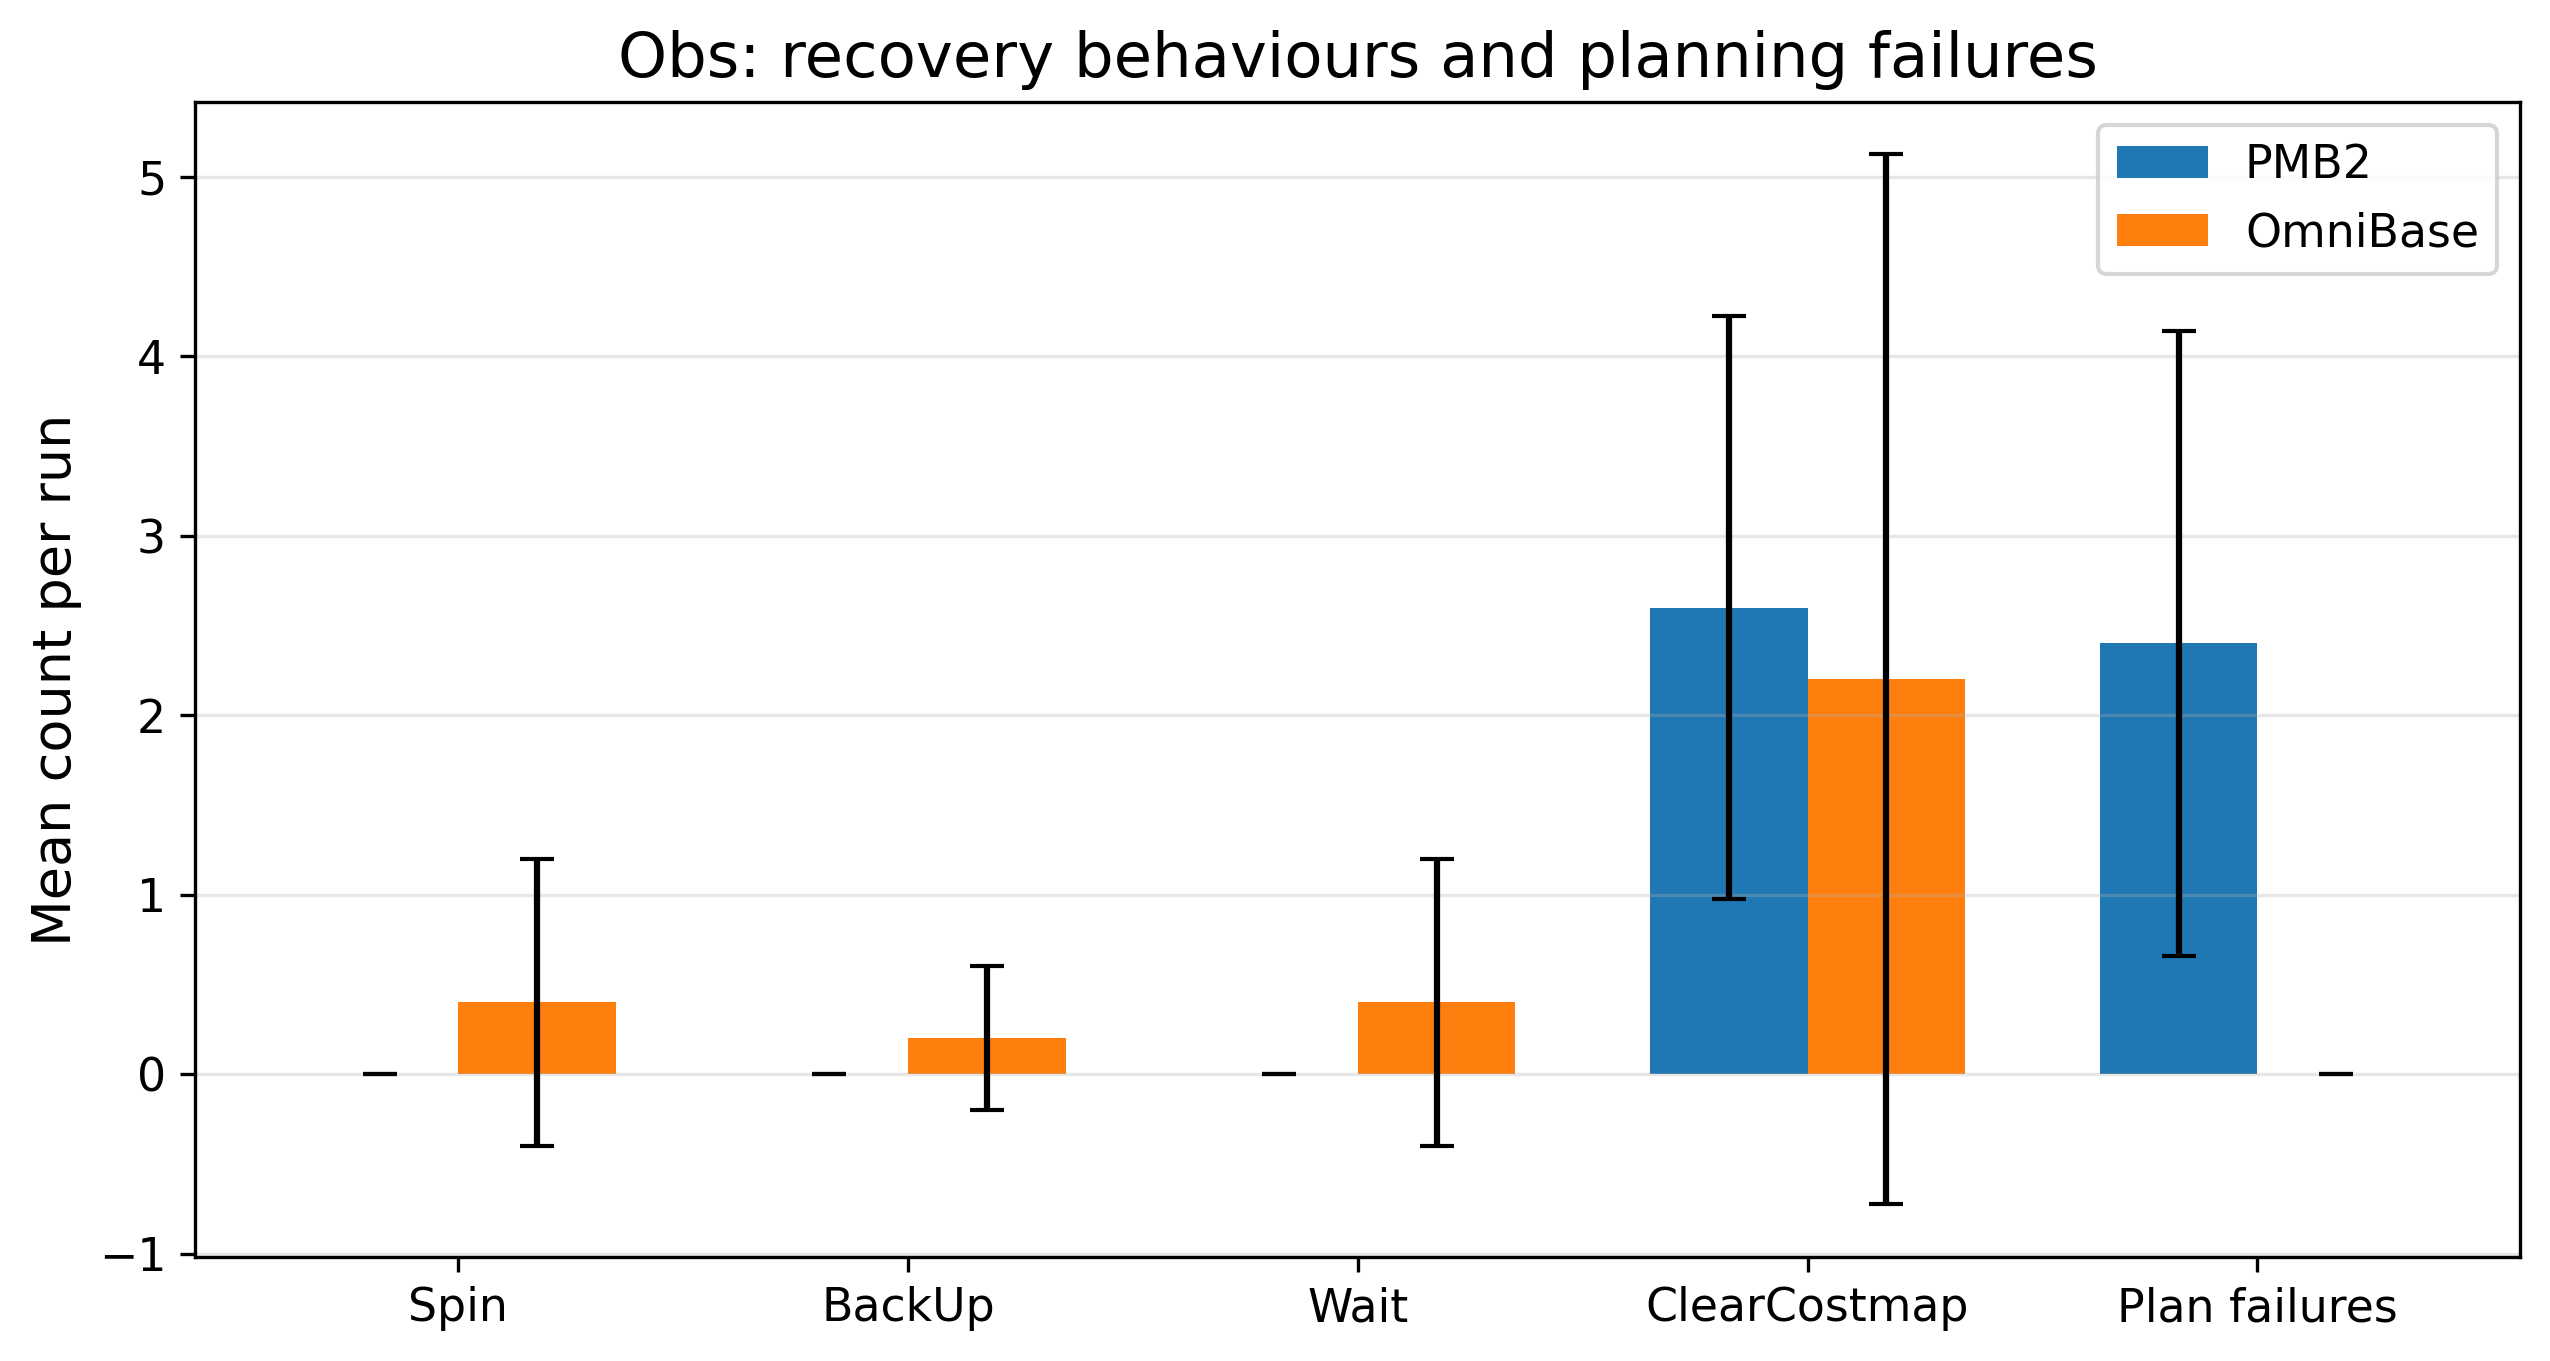
\includegraphics[width=0.9\textwidth]{images/Ch4/obs/recovery_counts_Obs.png}
  \caption{Cluttered obstacle course: recovery behaviours and planning failures, mean per run over five runs. The differential base fails to plan repeatedly (rightmost group) but never invokes Spin, BackUp, or Wait; the holonomic base never fails to plan, its few manoeuvre recoveries originating almost entirely from a single stuck run.}
  \label{fig:obs-recov}
\end{figure}

Figure~\ref{fig:obs-recovmap} reveals \emph{where} this struggle occurs. For the differential base the costmap-clearing actions are not scattered along the route but cluster at its tightest passage---the narrow section where the circuit doubles back close to its own starting point---indicating that the global planner repeatedly failed to route the non-holonomic footprint through that gap and had to clear the costmap and retry. The holonomic base cleared its costmap only once, at the same pinch point. This is the spatial fingerprint of the kinematic difference: at a narrow passage the holonomic base can side-step laterally into a valid trajectory, so a feasible plan is almost always found, whereas the differential base, which must rotate before it can translate, more often finds no admissible plan and falls back on the recovery pipeline.

\begin{figure}[H]
  \centering
  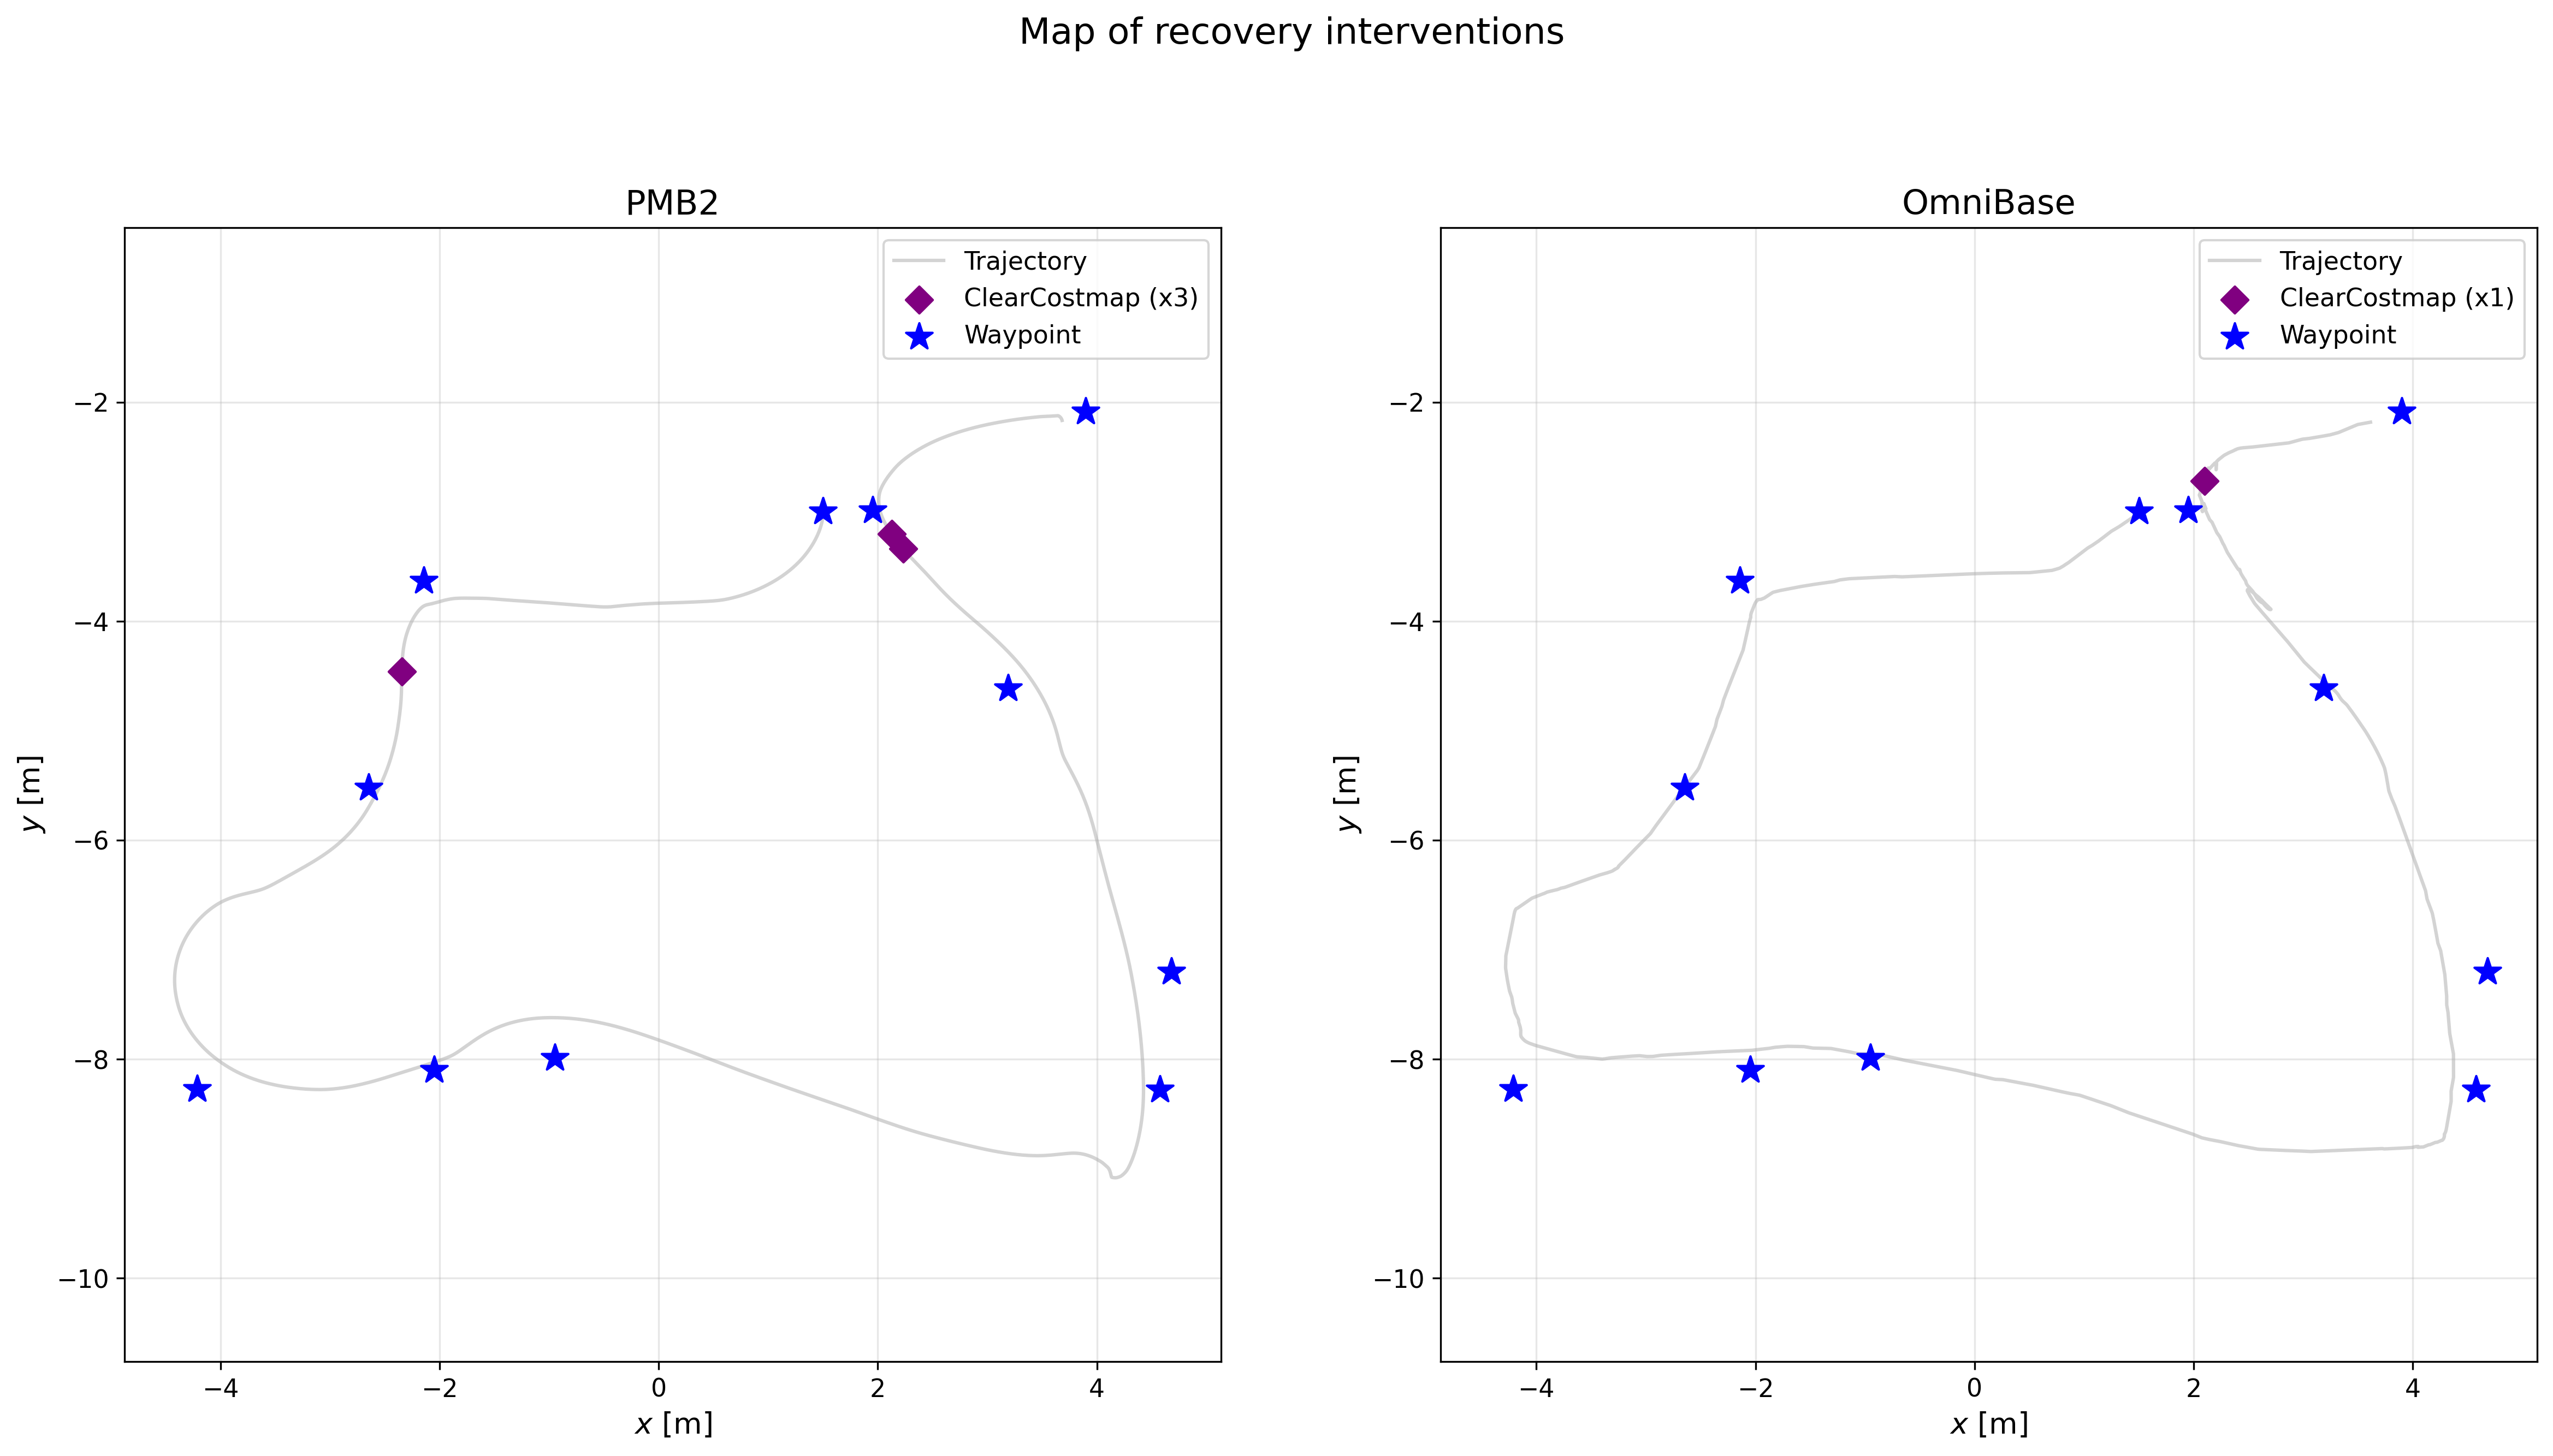
\includegraphics[width=\textwidth]{images/Ch4/obs/recovery_map.png}
  \caption{Cluttered obstacle course: location of the costmap-clearing actions for a representative run of each base (three for the PMB2, one for the OmniBase). The differential base's clears cluster at the narrowest passage of the circuit, where routing its footprint repeatedly failed.}
  \label{fig:obs-recovmap}
\end{figure}

\begin{figure}[H]
  \centering
  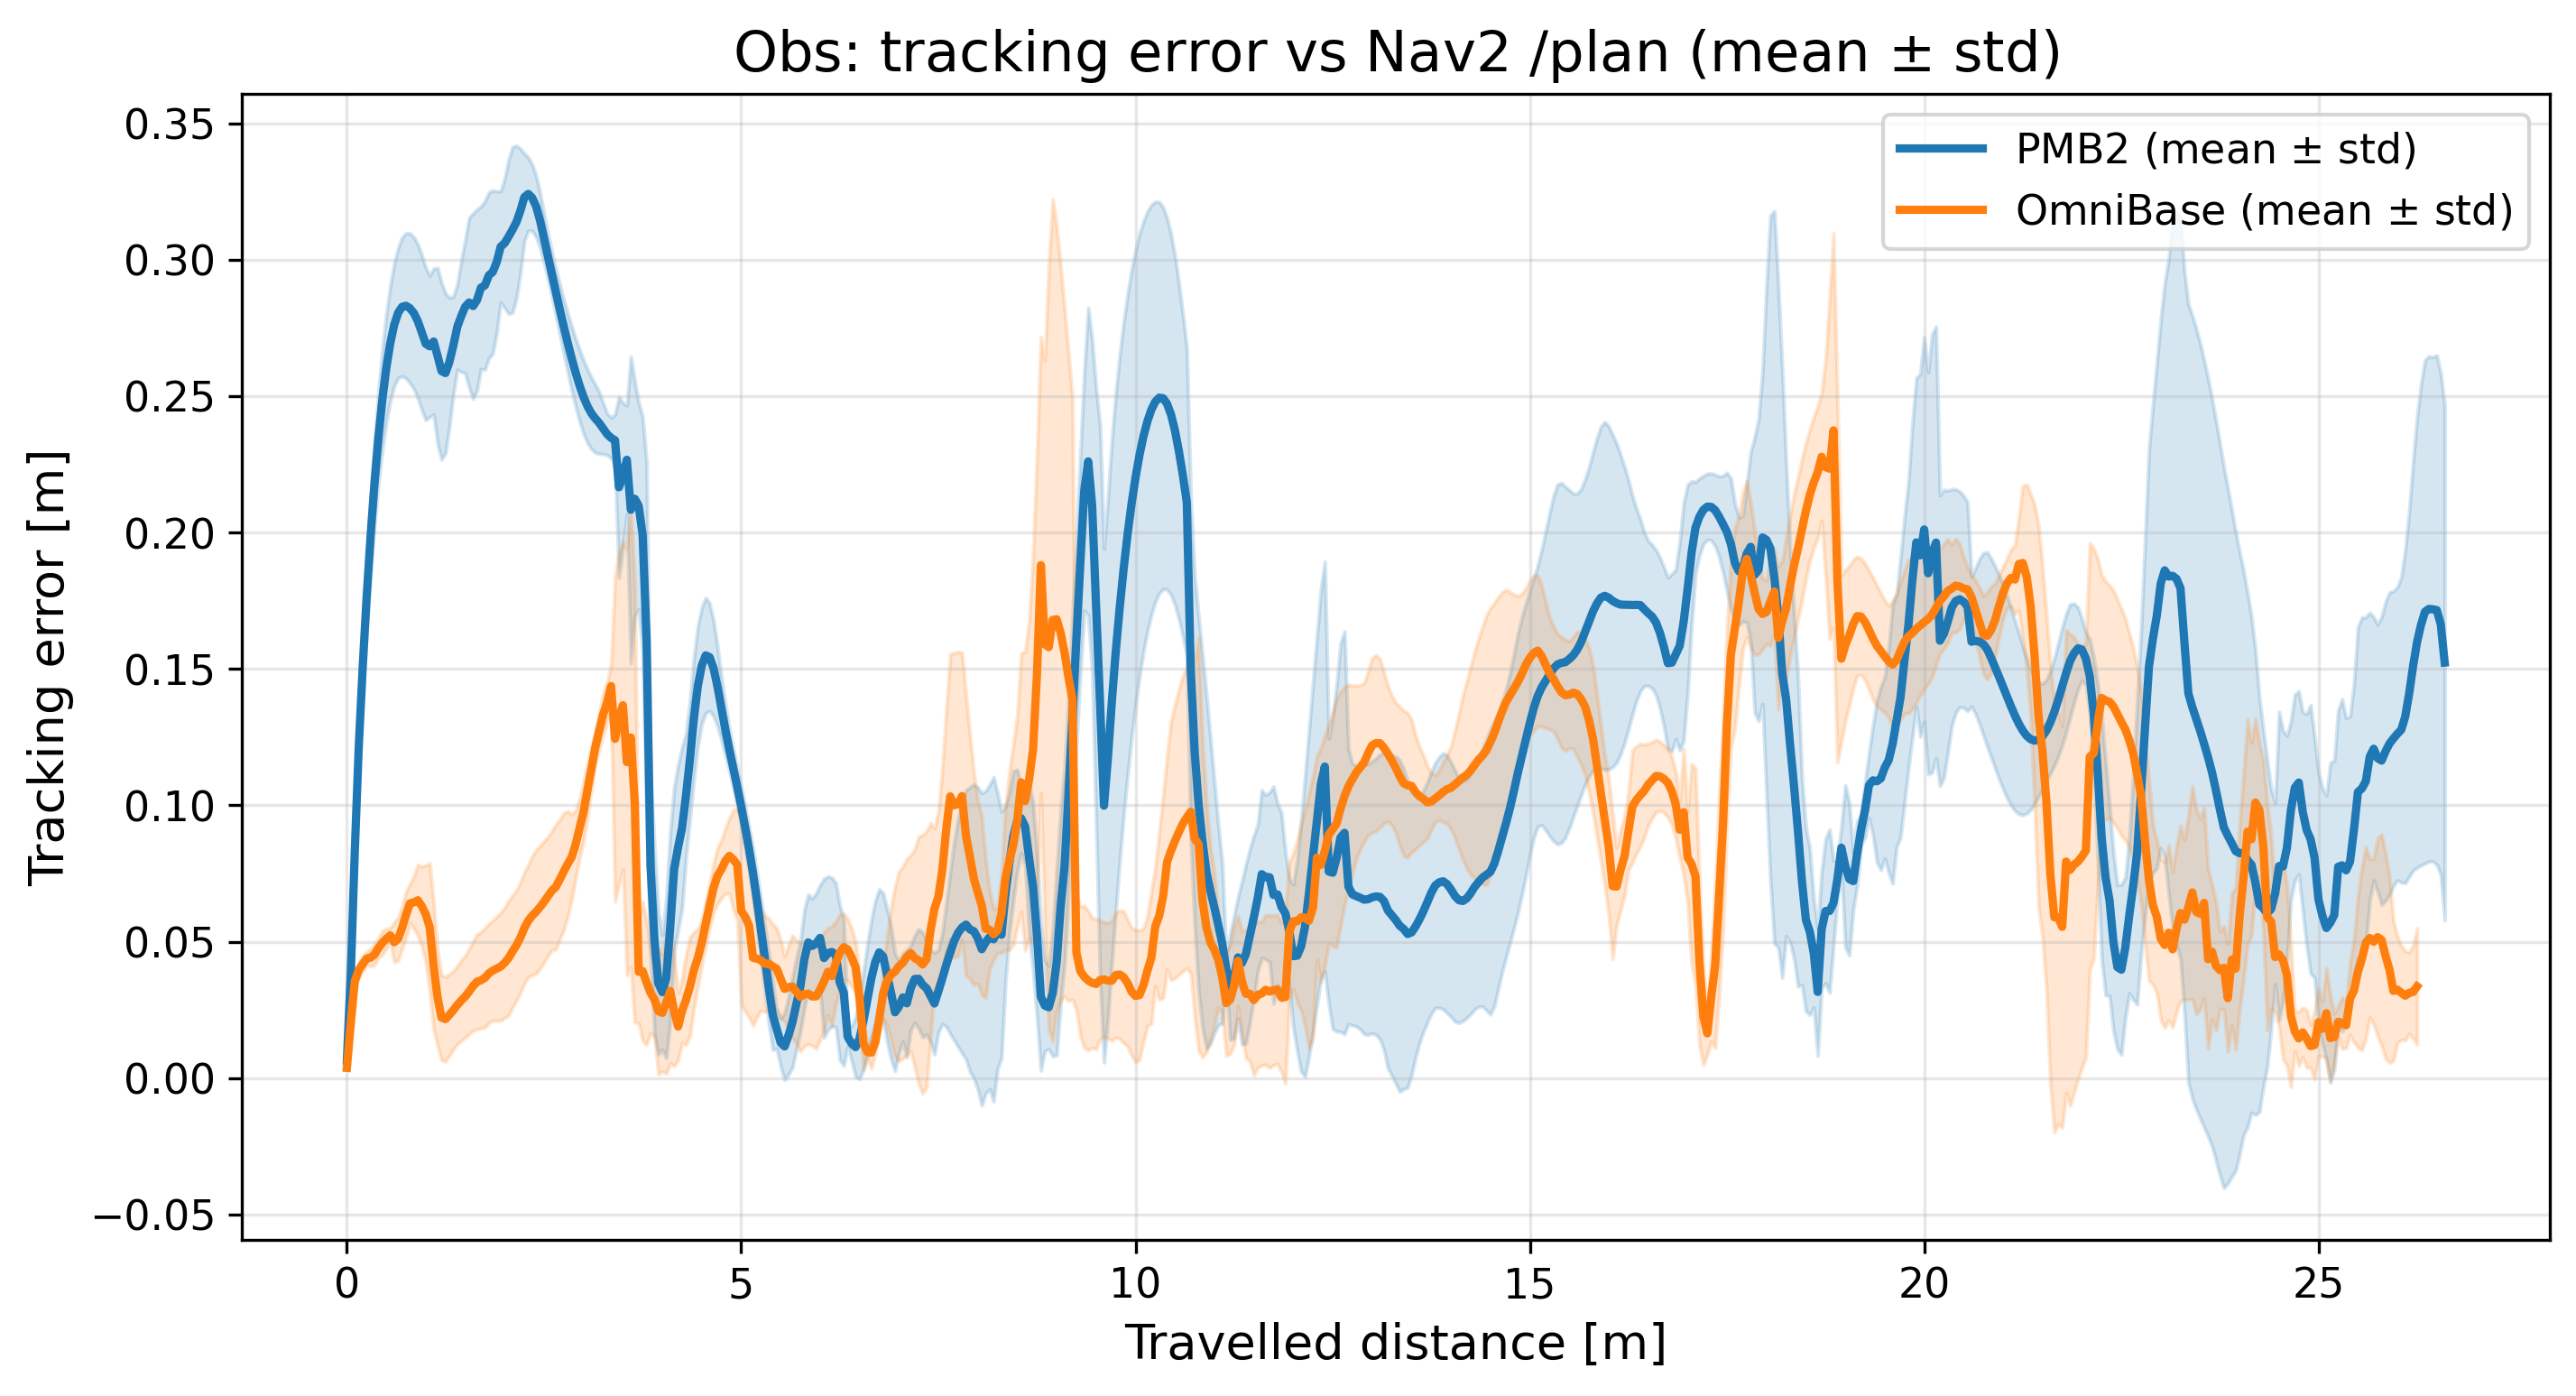
\includegraphics[width=1\textwidth]{images/Ch4/obs/cross_track_band_Obs.png}
  \caption{Cluttered obstacle course: tracking error against the Nav2 global plan as a function of travelled distance (mean $\pm$ standard deviation over five runs). Unlike the smooth growth observed on the straight corridor, both profiles are markedly jagged, reflecting the many tight manoeuvres the clutter demands; the holonomic OmniBase remains lower on average.}
  \label{fig:obs-xtrack}
\end{figure}

Beyond robustness, the route confirms the tracking and effort patterns seen earlier. As on the straight corridor, the holonomic base follows the planned path more closely on average (mean tracking error $0.068$ against $0.136$~m), correcting deviations laterally. As Figure~\ref{fig:obs-xtrack} shows, however, the tracking-error profiles of both bases are now markedly jagged---in contrast to the smooth accumulation seen on the corridor---reflecting the many tight manoeuvres the clutter demands. The waypoint positioning errors are comparable between the platforms ($0.175$ against $0.187$~m) and vary from waypoint to waypoint according to the local corner-cutting geometry, with no consistent winner. The clearest separation is in angular effort: over eleven waypoints the differential base is almost continuously re-orienting, which yields an angular smoothness more than twice as large as the holonomic base's ($2.833$ against $1.217$~rad/s$^2$) and a large mean orientation error ($1.670$~rad)---the latter again reflecting the constantly changing heading of a base that must turn in order to move, rather than a failure to reach commanded orientations (Section~\ref{subsec:m-accuracy}). The holonomic base instead holds its heading and relies on lateral motion (lateral usage $0.649$).

In summary, the obstacle course inverts the lesson of the sharp corner. There, holonomy bought speed; here, on a long cluttered route requiring frequent reorientation from both platforms, the completion times are comparable on the median and holonomy instead buys \emph{robustness}---no planning failures and tighter path adherence---together with far lower angular effort. The recurring theme is the fragility of the differential base's planning in confined spaces, a fragility that, as the next section shows, reappears in the autonomous-exploration pipeline. As throughout, the absolute smoothness and variance figures remain subject to the actuation-fidelity caveat of Section~\ref{subsec:m-fidelity}.

\section{Autonomous Exploration Results}
\label{sec:expl-results}

This section reports the autonomous frontier-based exploration of the \texttt{home} apartment, the second navigation pipeline of this study. Both platforms completed all five runs, each terminating on the frontier-exhaustion criterion of Section~\ref{subsec:expl-protocol} after mapping essentially the whole apartment. The outcome is more nuanced than a simple ordering: as summarised in Table~\ref{tab:explore}, the two bases reach an equivalent final coverage, but the differential PMB2 covers the environment faster and more efficiently, while the holonomic OmniBase is far more robust in planning and more stable in localisation. The planning fragility already observed on the cluttered waypoint route (Section~\ref{subsec:res-obstacles}) reappears here in an even more pronounced form.

\begin{table}[htbp]
\centering
\caption{Autonomous exploration: aggregate metrics, mean $\pm$ standard deviation over five runs.}
\label{tab:explore}
\begin{tabular}{lcc}
\toprule
Metric & PMB2 (differential) & OmniBase (holonomic) \\
\midrule
Exploration time [s]           & $281.2 \pm 14.1$ & $365.0 \pm 48.3$ \\
Time to target area [s]        & $224.4 \pm 40.1$ & $315.6 \pm 43.7$ \\
Final mapped area [m$^2$]      & $255.7 \pm 2.8$ & $250.1 \pm 1.8$ \\
Path length [m]                & $58.3 \pm 11.5$ & $61.7 \pm 9.1$ \\
Efficiency [m$^2$/m]           & $4.52 \pm 0.68$ & $4.13 \pm 0.54$ \\
Efficiency [m$^2$/s]           & $0.91 \pm 0.05$ & $0.70 \pm 0.11$ \\
SLAM error, mean [m]           & $0.176 \pm 0.122$ & $0.096 \pm 0.012$ \\
SLAM error, max [m]            & $0.391 \pm 0.236$ & $0.239 \pm 0.042$ \\
Angular smoothness [rad/s$^2$] & $2.247 \pm 0.158$ & $1.220 \pm 0.044$ \\
Lateral usage                   & $0.000 \pm 0.000$ & $0.579 \pm 0.044$ \\
Planning failures              & $32.4 \pm 19.8$ & $0.0 \pm 0.0$ \\
Costmap clears                 & $24.4 \pm 11.6$ & $11.4 \pm 5.2$ \\
Spin / BackUp / Wait           & $3.8$ / $2.0$ / $3.0$ & $1.6$ / $0.2$ / $1.0$ \\
\bottomrule
\end{tabular}
\end{table}

\begin{figure}[H]
  \centering
  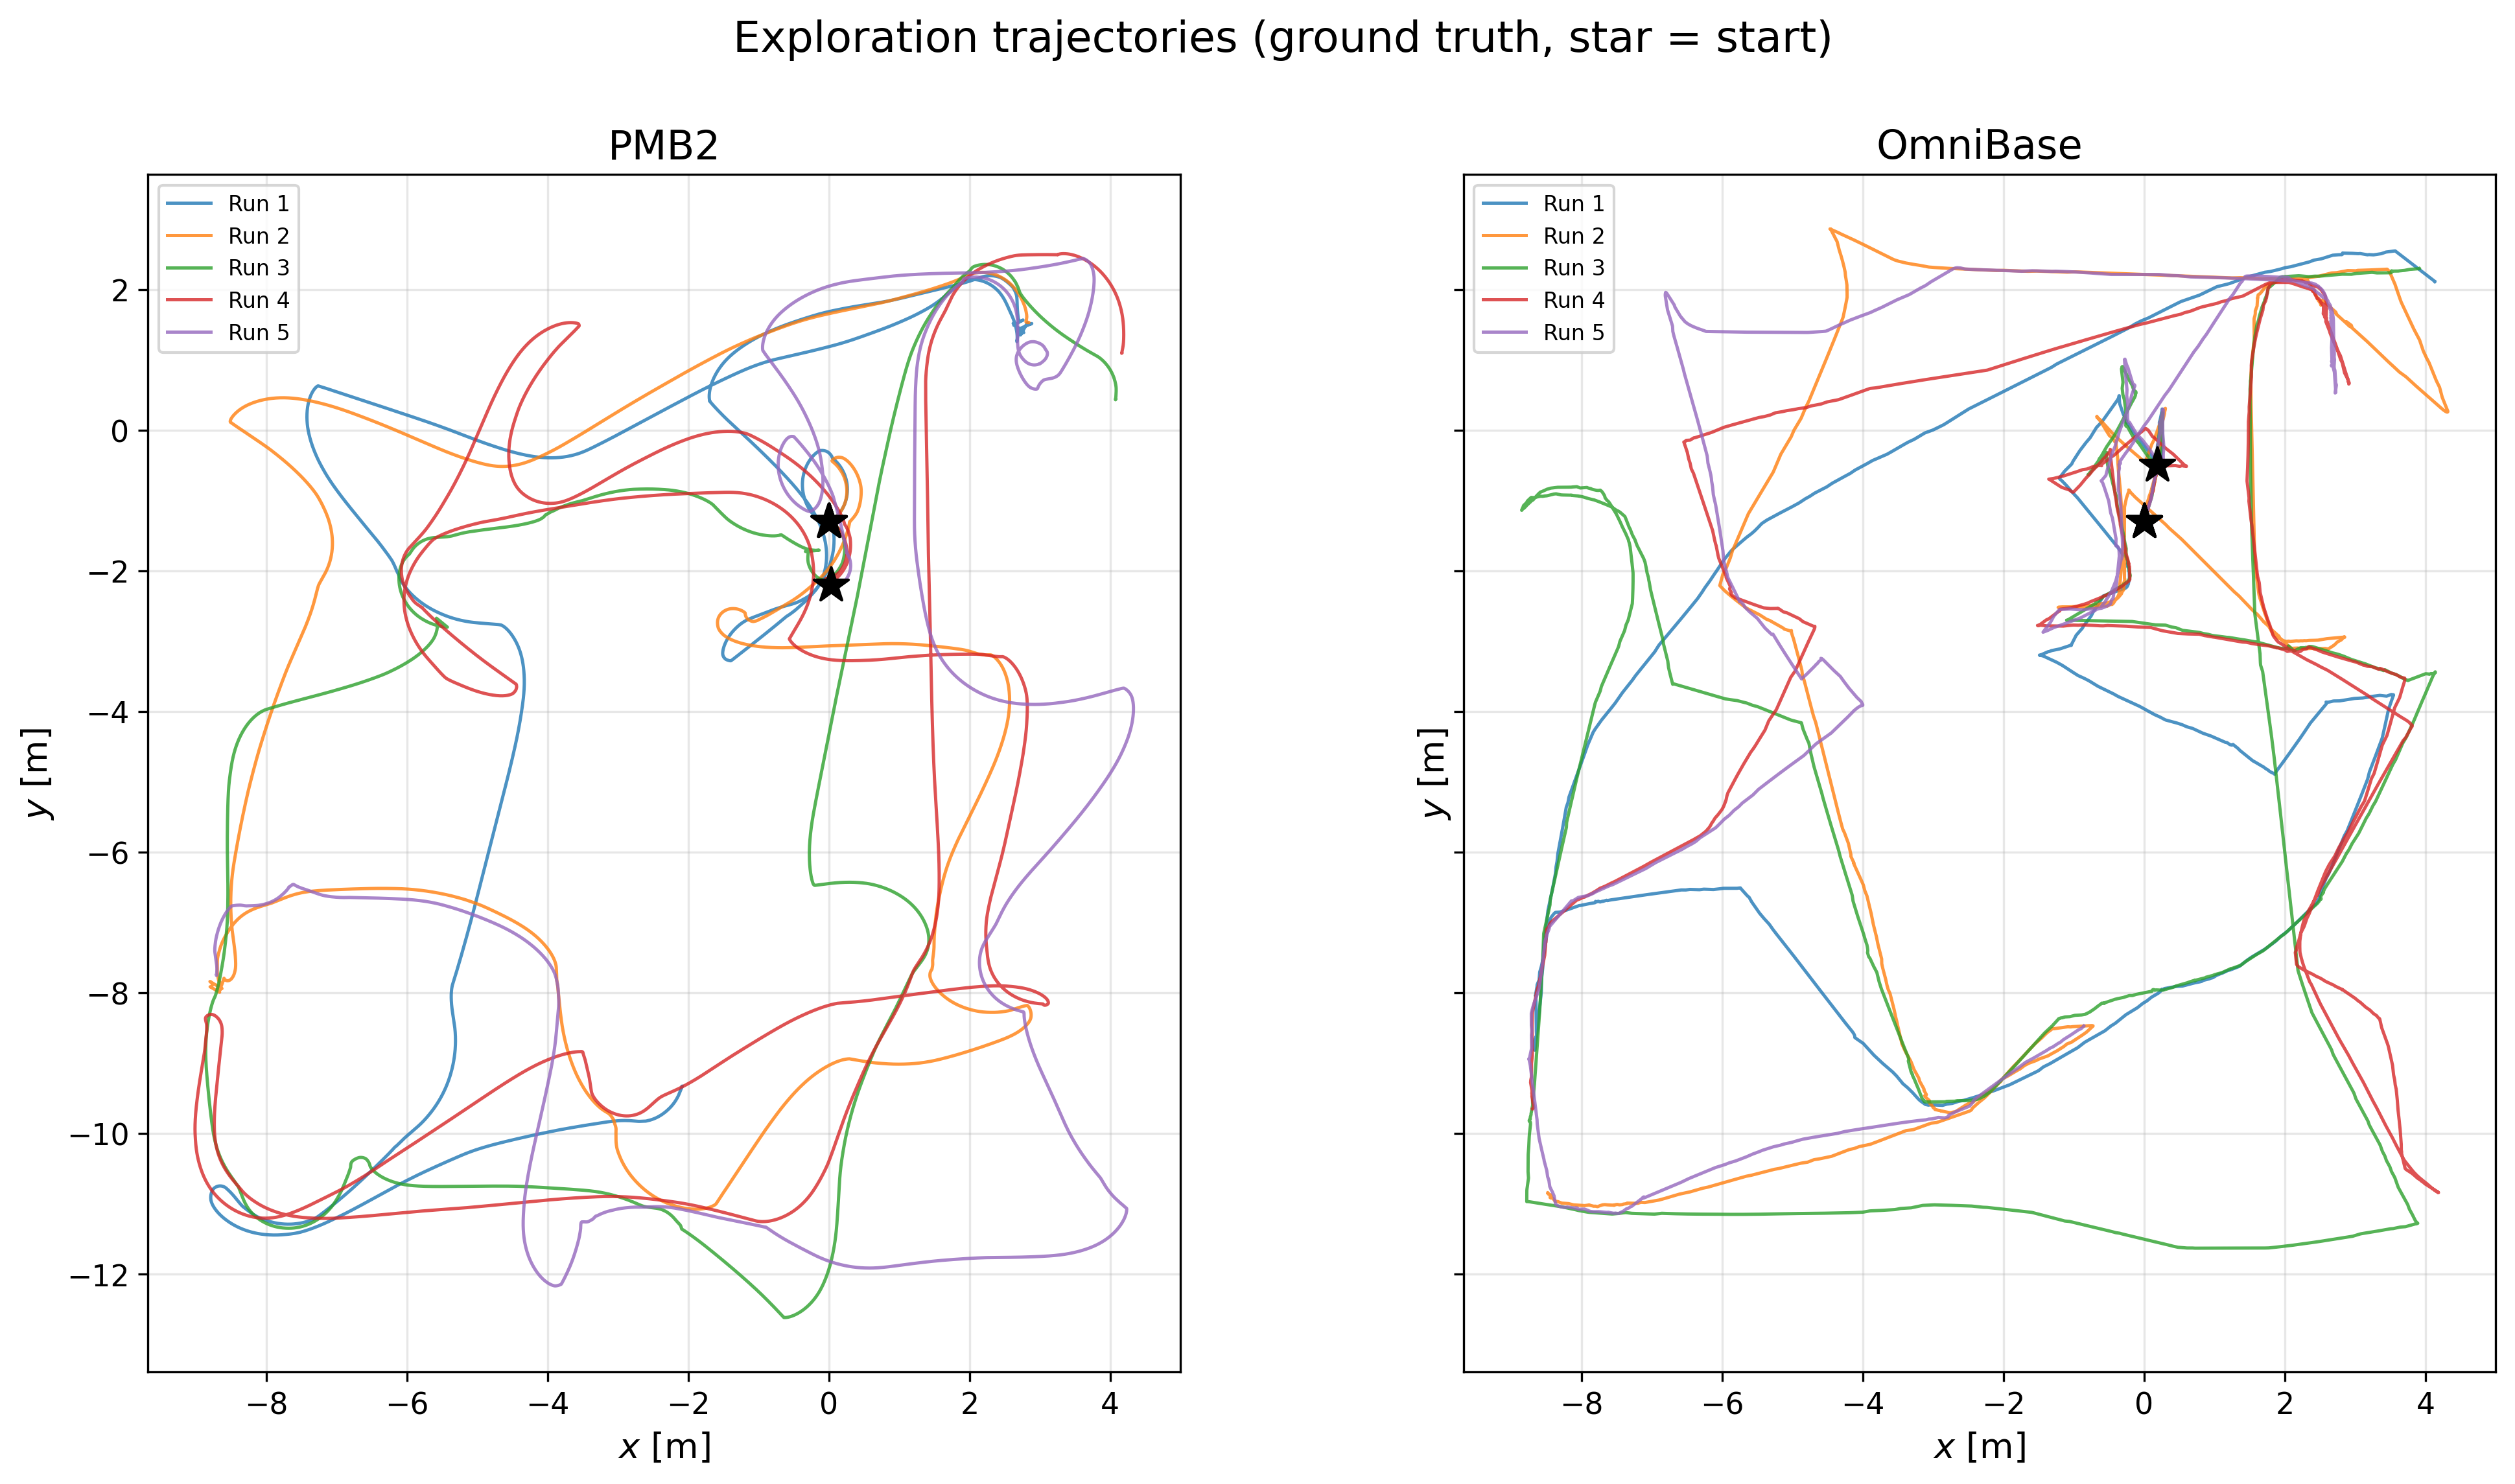
\includegraphics[width=\textwidth]{images/Ch4/expl/exploration_trajectories.png}
  \caption{Autonomous exploration: Ground~Truth trajectories of all five runs per base (stars mark the start pose). Both platforms traverse the entire apartment; the paths differ markedly from run to run, as expected from the frontier-selection process, which discovers and visits regions in a different order each time.}
  \label{fig:expl-traj}
\end{figure}

Figure~\ref{fig:expl-traj} shows that both platforms explore the whole apartment, and that---unlike the waypoint routes---the trajectories are not repeatable across runs: since the next goal depends on the frontiers currently visible in the incrementally built map, each run discovers the environment along a different path. This run-to-run variability is intrinsic to the task rather than a symptom of instability, and it is the reason the exploration campaign is characterised statistically over five repetitions.

\begin{figure}[H]
  \centering
  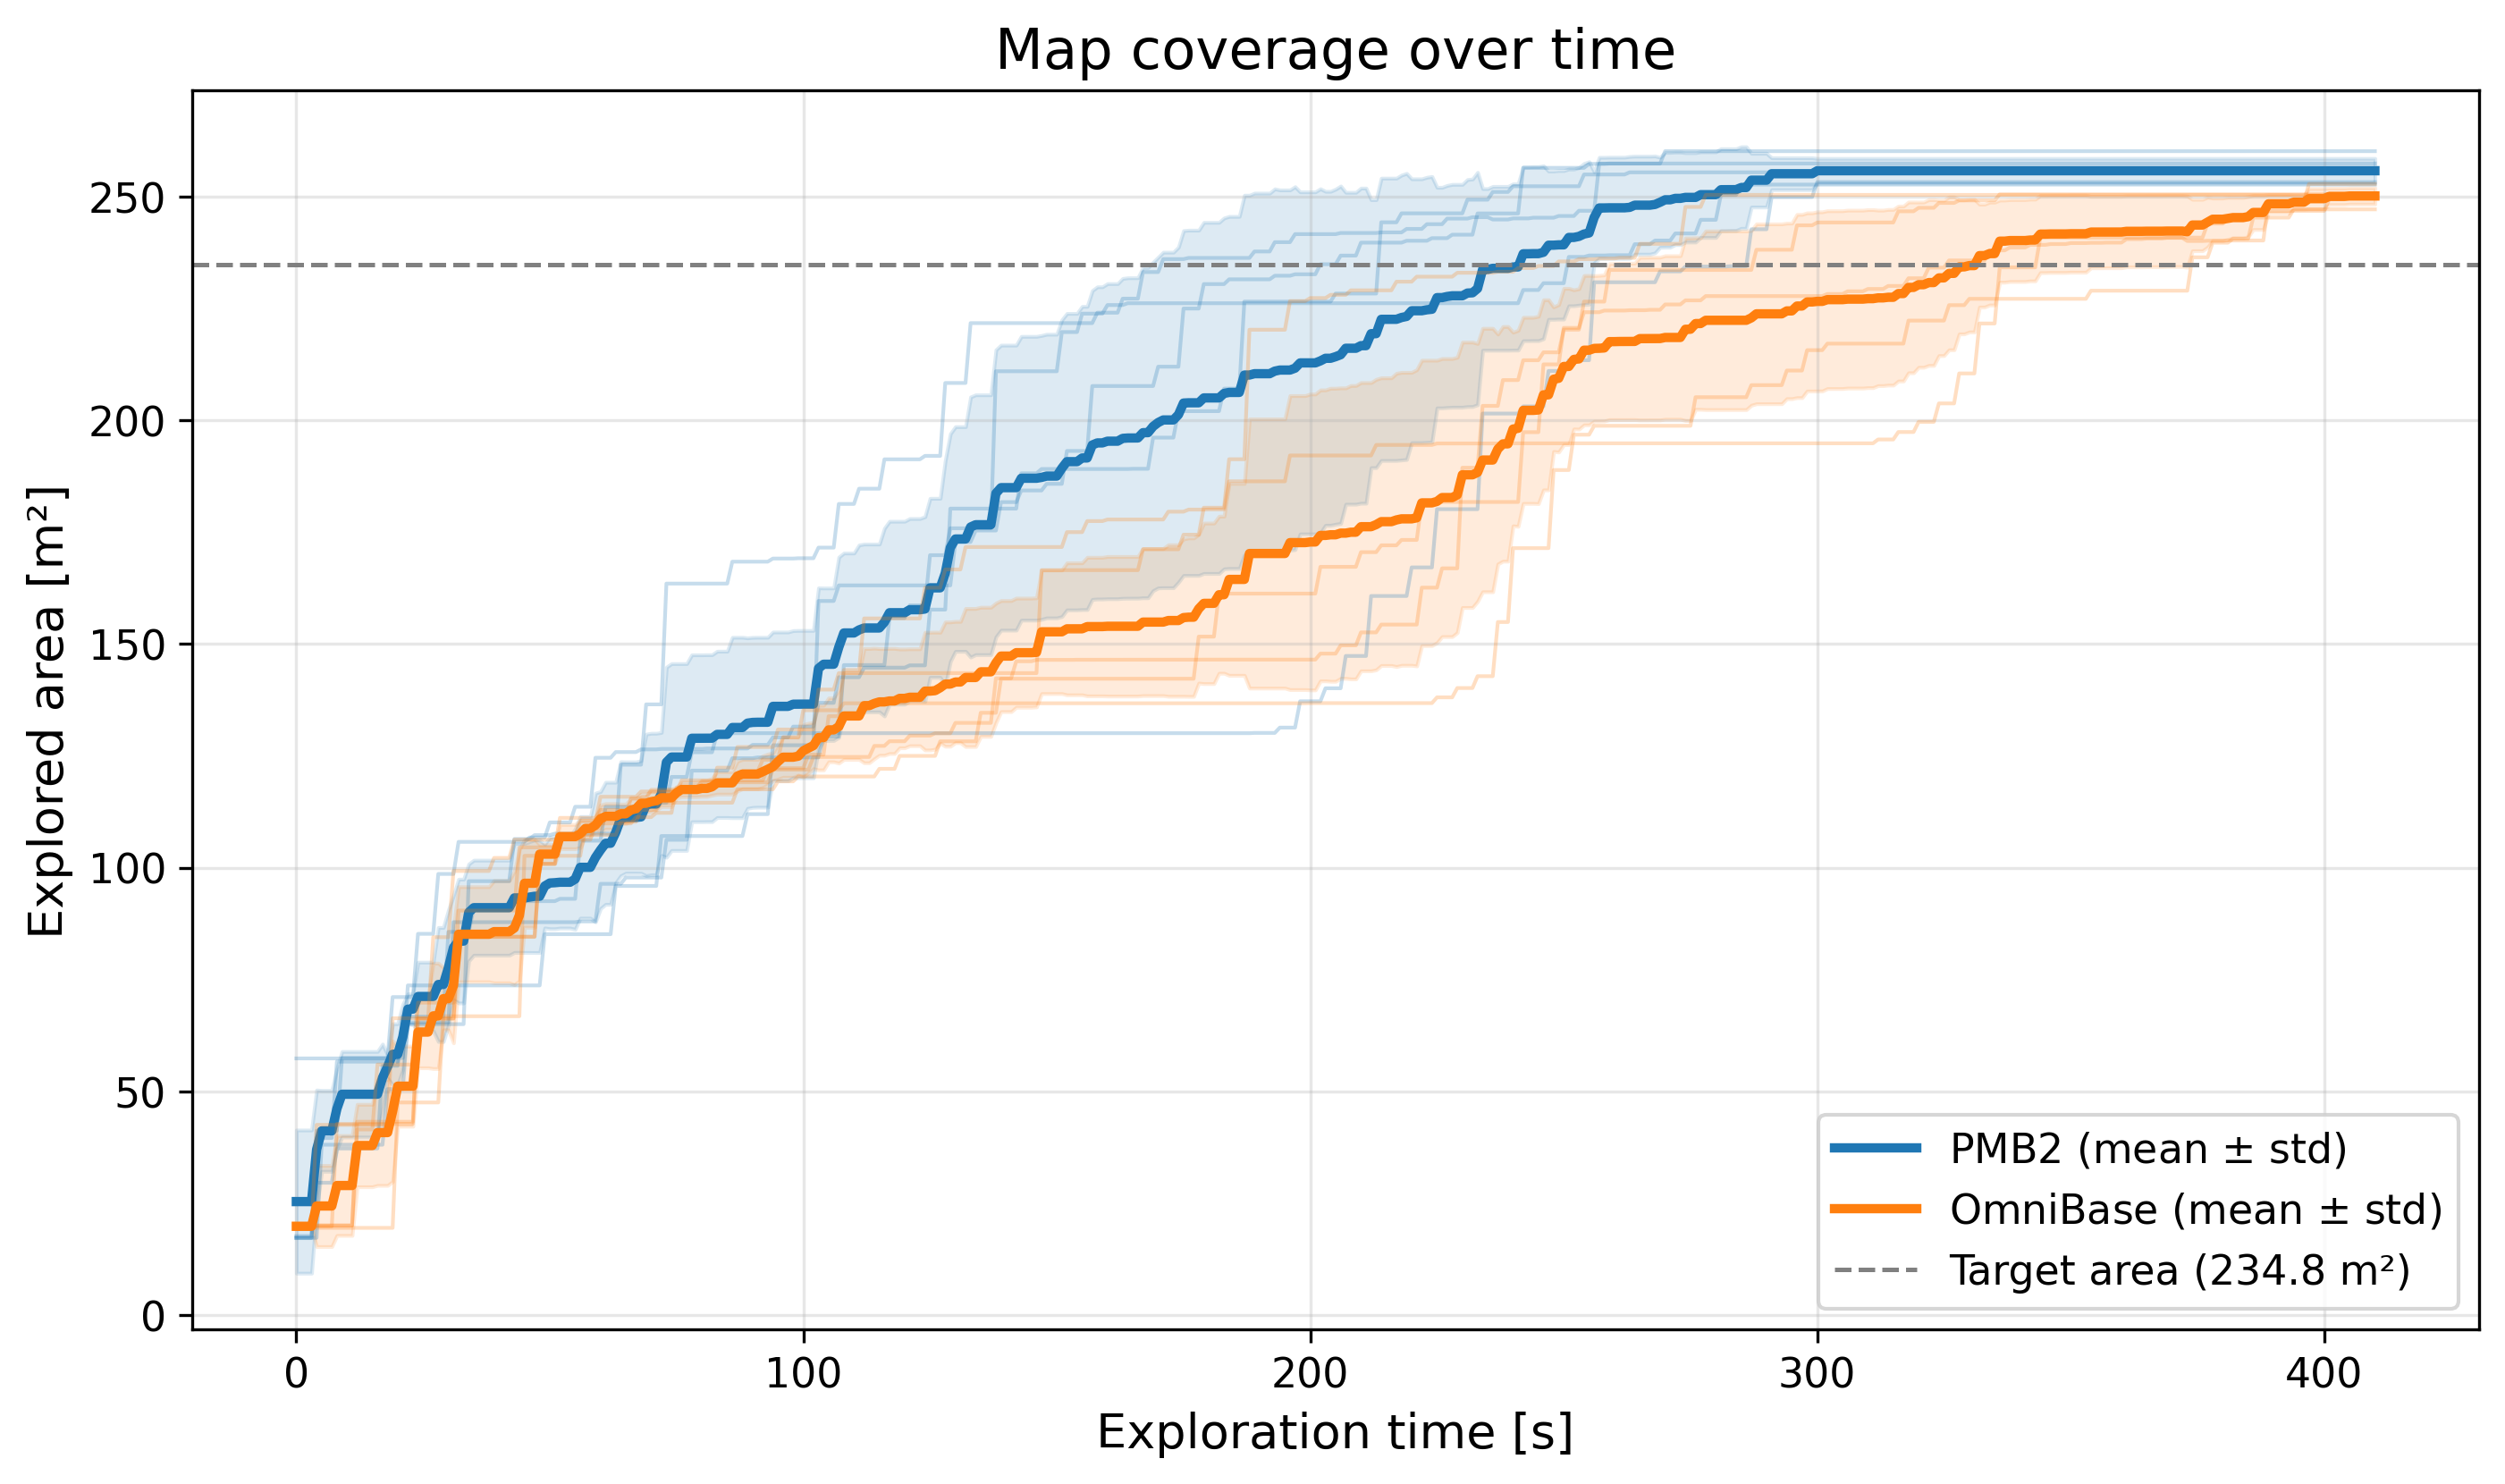
\includegraphics[width=1\textwidth]{images/Ch4/expl/coverage_vs_time.png}
  \caption{Autonomous exploration: mapped area as a function of exploration time (mean $\pm$ standard deviation over five runs). The differential PMB2 reaches the common target coverage (dashed line, $234.8$~m$^2$, i.e.\ $95\%$ of the smallest final area) earlier than the holonomic OmniBase; both converge to a similar final mapped area.}
  \label{fig:expl-coverage}
\end{figure}

In terms of coverage the differential base is the more effective of the two. Figure~\ref{fig:expl-coverage} shows its mapped area growing consistently faster: it reaches the common target coverage in $224$~s on average, against $316$~s for the holonomic base, and completes the whole exploration in $281$~s against $365$~s. The differential is also more efficient by both measures, covering more area per metre travelled ($4.52$ against $4.13$~m$^2$/m) and per second ($0.91$ against $0.70$~m$^2$/s), while the two platforms end at an equivalent final area ($255.7$ against $250.1$~m$^2$). This inverts the speed relationship seen at the sharp corner (Section~\ref{subsec:res-angle}). The reason lies in the geometry that the two bases must follow while mapping: much of the exploration consists of tracing long, narrow paths that skirt the apartment walls, often as elongated ``U''-shaped detours around a wall or into and out of a room. The differential PMB2, with its round footprint, negotiates such contours as wide, sweeping curves and traverses them quickly; the holonomic OmniBase, by contrast, has no manoeuvre to exploit along a wall---sideways motion offers no shortcut there---and its finer, closely-guided wall-following is comparatively slow. Since the open apartment rewards fast contour-following far more than lateral agility, the differential base covers the same area appreciably faster, while both reach an equivalent final extent. Figure~\ref{fig:expl-coverage} also shows that this gap does not open immediately: during the first $\sim$100~s the two coverage curves are almost indistinguishable, and the differential base pulls ahead only in the intermediate phase. This is consistent with the wall-following interpretation, as the initial coverage comes from the open central rooms---which both bases map at a similar rate---whereas the divergence appears once the exploration moves into the narrower, wall-bounded portions of the apartment that penalise the holonomic base.

\begin{figure}[H]
  \centering
  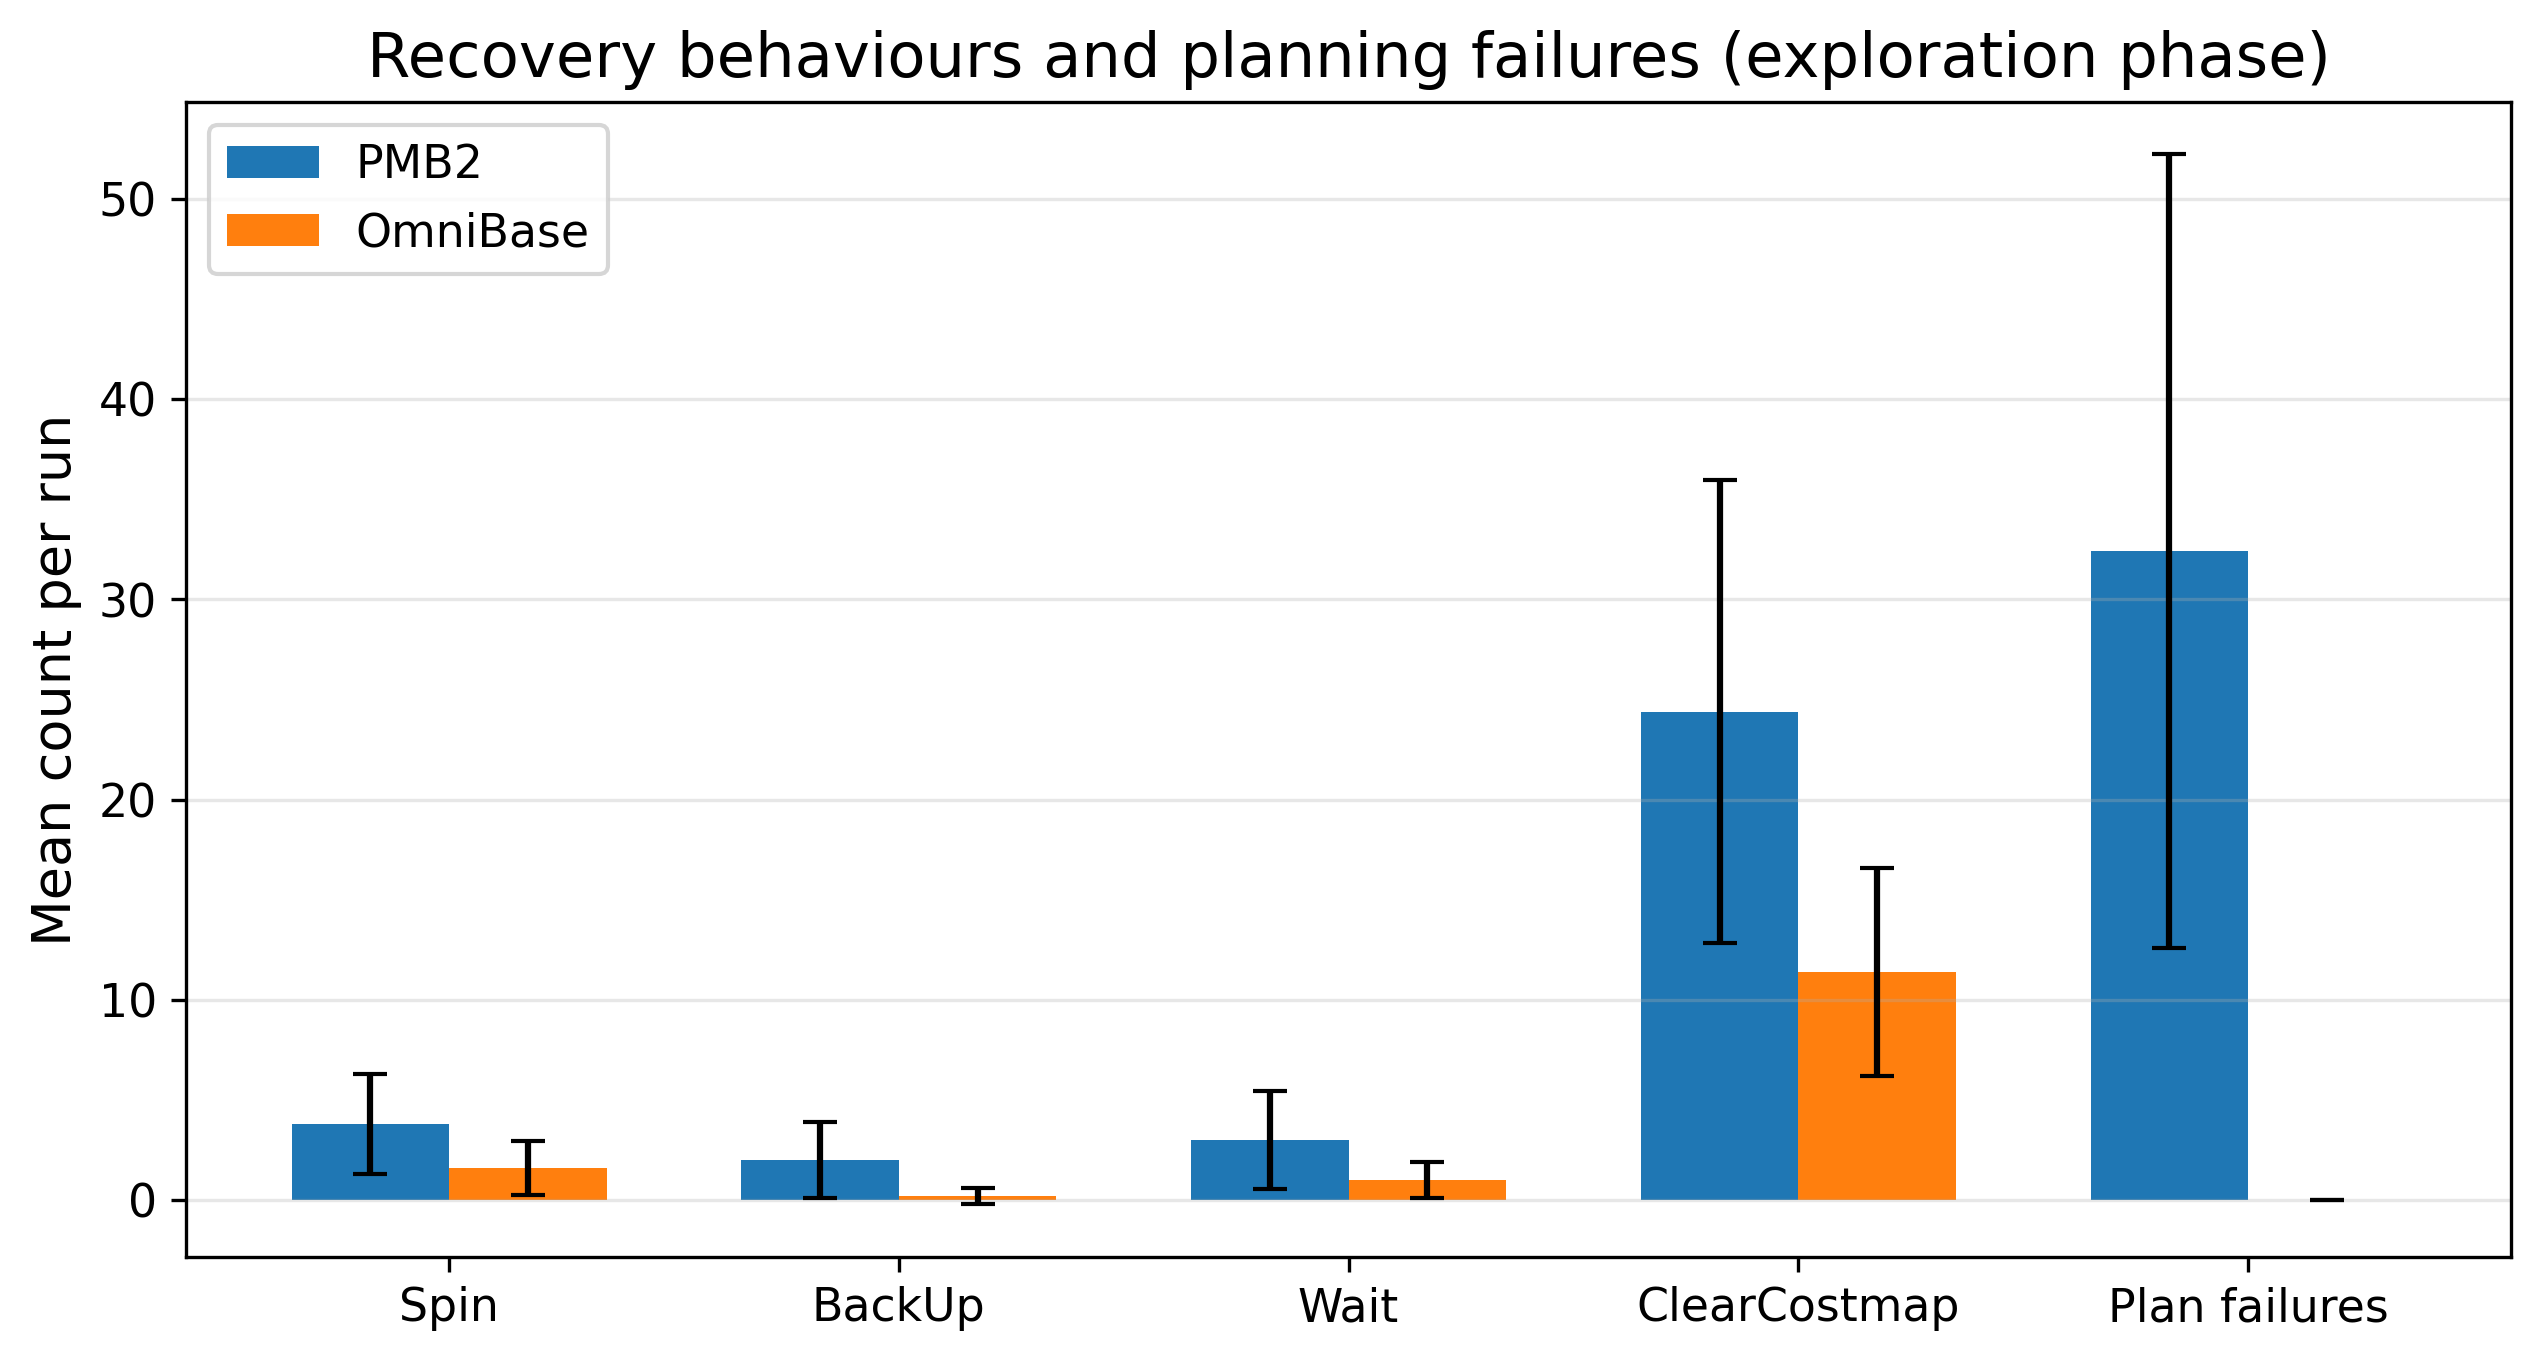
\includegraphics[width=1\textwidth]{images/Ch4/expl/recovery_counts.png}
  \caption{Autonomous exploration: recovery behaviours and planning failures, mean per run over five runs. The differential PMB2 incurs a large number of planning failures ($32.4$ per run on average) and more of every recovery action, whereas the holonomic OmniBase never fails to plan.}
  \label{fig:expl-recov}
\end{figure}

This coverage advantage, however, is bought at a steep price in robustness, and it is here that the central theme of the waypoint campaign re-emerges. As Figure~\ref{fig:expl-recov} shows, the differential base failed to produce a valid global plan an average of $32.4$ times per run---about $6\%$ of its planning attempts---while the holonomic base never failed once. The differential also triggered more of every recovery action, in particular clearing its costmap more than twice as often ($24.4$ against $11.4$). The mechanism is the same as on the obstacle course: the apartment mixes open rooms, which the differential crosses quickly, with narrow inter-room passages and doorways, through which routing a non-holonomic footprint repeatedly fails, forcing a costmap clear and a replan. The holonomic base negotiates the same passages by side-stepping into a feasible trajectory and therefore never exhausts the planner. Notably, these failures cost the differential time but not enough to erase its locomotion advantage: it still completes exploration faster despite recovering far more often.

\begin{figure}[H]
  \centering
  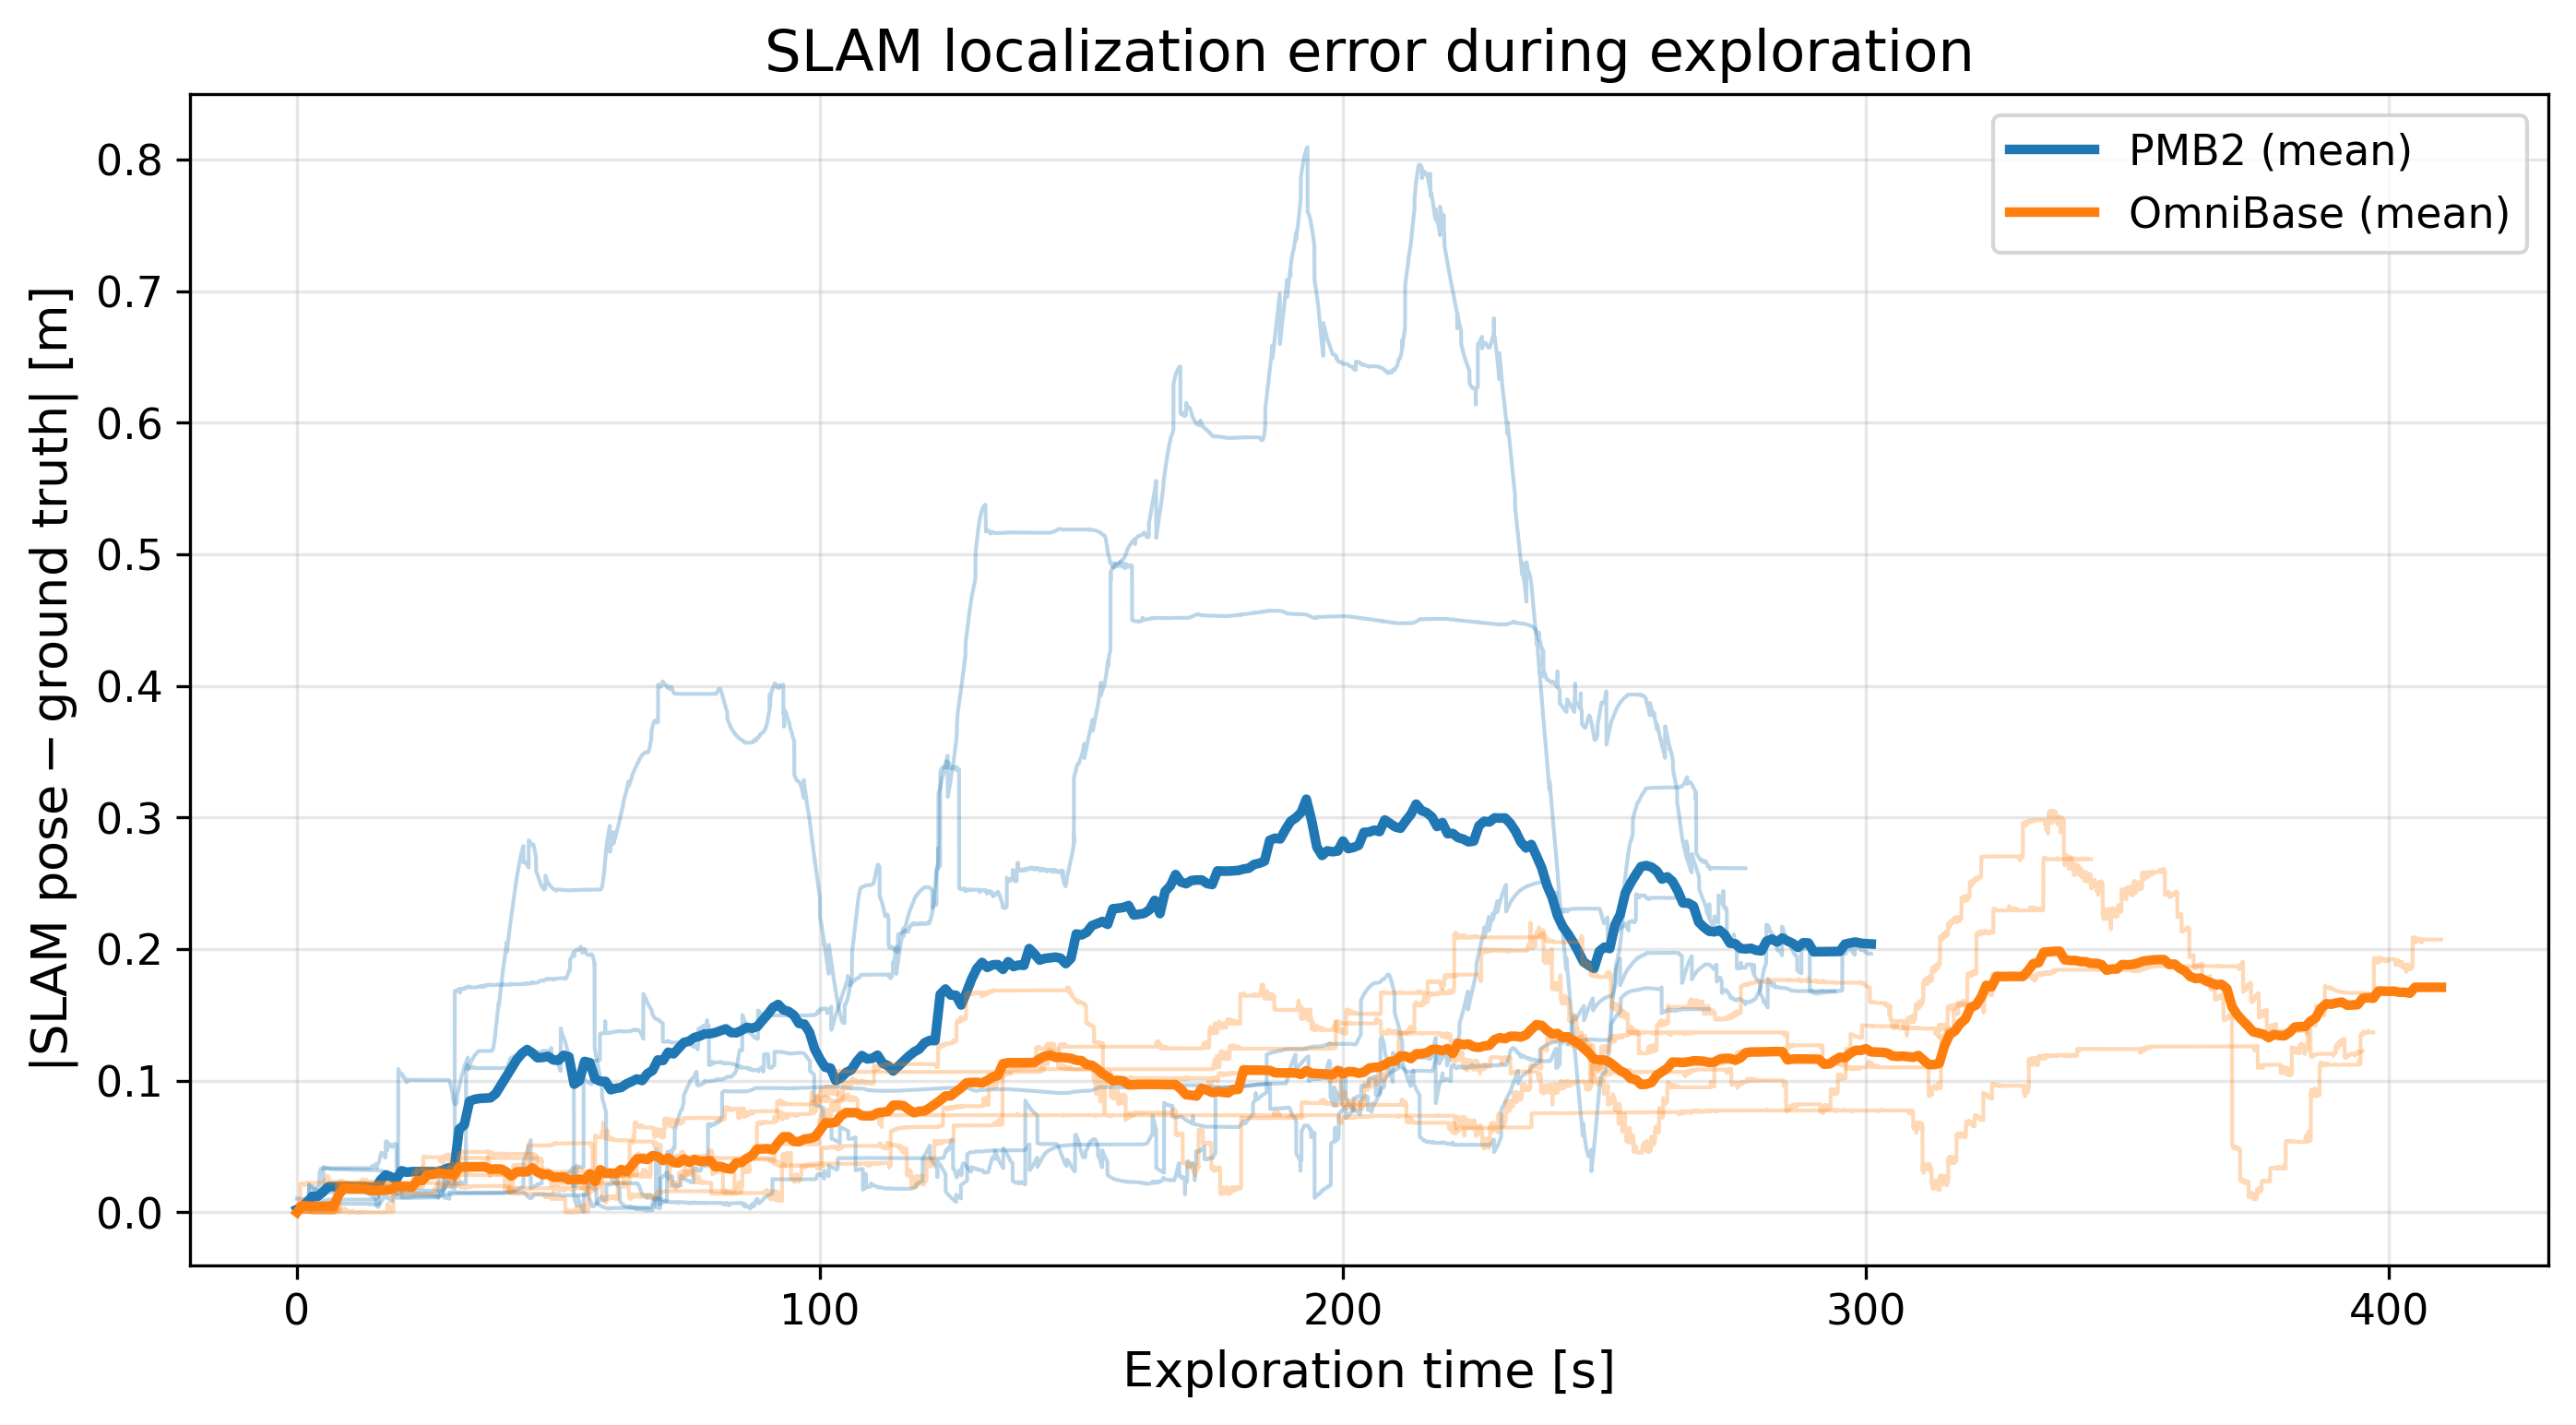
\includegraphics[width=1\textwidth]{images/Ch4/expl/slam_error_vs_time.png}
  \caption{Autonomous exploration: SLAM localisation error (distance between the \texttt{slam\_toolbox} estimate and Ground~Truth) over exploration time; bold lines are the per-base mean, faint lines the individual runs, after the map-to-world alignment of Section~\ref{subsec:m-exploration}. The holonomic OmniBase maintains a lower and far more consistent error, whereas the differential PMB2 is higher and highly variable, one run exceeding $0.8$~m. The OmniBase curves extend later in time, reflecting its longer exploration duration.}
  \label{fig:expl-slam}
\end{figure}

The second cost concerns localisation. Figure~\ref{fig:expl-slam} reports the error of the online SLAM estimate against Ground~Truth, after the per-run frame alignment described in Section~\ref{subsec:m-exploration}. The holonomic base maintains a low and remarkably consistent error (mean $0.096 \pm 0.012$~m), its five runs tightly bunched throughout. The differential base is both less accurate and dramatically less consistent (mean $0.176 \pm 0.122$~m, with a standard deviation almost as large as the mean): its error grows more steeply and its runs fan out widely, one exceeding $0.8$~m at its peak. Since both platforms run the same \texttt{slam\_toolbox} configuration, this difference reflects the interaction between the SLAM front-end and the two odometric regimes rather than a property of the mapping algorithm itself (Section~\ref{subsec:m-exploration}); the frequent in-place rotations of the differential base, and the drift they induce, are the most plausible source of its larger and more erratic localisation error, consistent with its markedly higher angular effort ($2.247$ against $1.220$~rad/s$^2$). This outcome may appear to run counter to the probabilistic analysis of Section~\ref{sec:probabilistic_motion_models}, which anticipated a broader, omnidirectional odometric uncertainty for the holonomic base and a more tightly constrained one for the differential. Two factors reconcile the two. First, that analysis concerns the raw odometric noise, whereas the error reported here is that of the full SLAM estimate: the additional lateral variance predicted for the OmniBase is precisely what the dedicated \texttt{alpha5} coefficient introduced in Section~\ref{subsec:amcl_tuning} is meant to bound. Second, and more decisively, what the scan-matching front-end of \texttt{slam\_toolbox} sees is the executed motion, and the OmniBase moves through long, smooth, heading-stable translations that are inherently favourable to registration, whereas the differential base interleaves its motion with the continual in-place rotations that its kinematics demand—the dominant source of pose drift for a laser SLAM system. The idealised, slip-free actuation of the OmniBase in simulation (Section~\ref{subsec:m-fidelity}) reinforces this effect and should be kept in mind: on physical hardware the lateral slippage of the Mecanum rollers would inject exactly the coupled noise that Section~\ref{sec:probabilistic_motion_models} describes, and the localisation gap would be expected to narrow.

In summary, the exploration pipeline does not crown a single winner but exposes a clear division of strengths. The differential PMB2 covers the apartment faster and more efficiently, benefiting from the ease with which its round footprint sweeps the wall-following contours that dominate the task; the holonomic OmniBase, though slower to explore, is decisively more robust---never failing to plan---and holds a substantially lower and more stable localisation error. Both map the environment to the same final extent. Crucially, the result that carries across both experimental campaigns is the differential base's planning fragility in confined spaces, which reappears in exploration in its most pronounced form. As throughout the chapter, the smoothness, variance, and localisation figures should be read in the light of the actuation-fidelity considerations of Section~\ref{subsec:m-fidelity}. These findings are drawn together into an overall comparison in Section~\ref{sec:comparative-discussion}.

\section{Comparative Analysis and Discussion}
\label{sec:comparative-discussion}

The two navigation paradigms have been benchmarked across two pipelines and four scenarios: three waypoint routes of increasing difficulty and an autonomous exploration of an unknown apartment. Taken together, the results do not identify a universally superior kinematics; rather, the advantage of each platform is strongly dependent on the task, and in several respects the ranking reverses from one scenario to the next. A single thread, however, runs consistently through both pipelines. Table~\ref{tab:summary} summarises the comparison, which the remainder of this section discusses by theme.

\begin{table}[htbp]
\centering
\caption{Cross-scenario summary of the comparison. Each cell reports the favoured platform on the given criterion; $\approx$ denotes comparable performance, and -- denotes a criterion not measured in that scenario.}
\label{tab:summary}
\vspace{0.3cm}
\begin{tabular}{lcccc}
\toprule
Criterion & Corridor (A) & Corner (B) & Obstacles (C) & Exploration \\
\midrule
Completion speed         & $\approx$ & OmniBase & $\approx$ & PMB2 \\
Path tracking (vs plan)  & OmniBase & PMB2 & OmniBase & -- \\
Planning robustness      & $\approx$ & $\approx$ & OmniBase & OmniBase \\
Angular effort (lower)   & $\approx$ & OmniBase & OmniBase & OmniBase \\
Localisation stability   & -- & -- & -- & OmniBase \\
\bottomrule
\end{tabular}
\end{table}

\subsection{Speed and Manoeuvrability}
\label{subsec:disc-speed}

The faster platform is not a property of the kinematics but of the interaction between the kinematics and the geometry of the task. At the sharp corner the holonomic OmniBase is almost three times faster than the differential PMB2, because it resolves the turn with a single lateral strafe while the differential must rotate to align, translate, and finally rotate again to meet the commanded goal orientation. In autonomous exploration the relationship inverts: the differential base covers the apartment appreciably faster (reaching the target coverage in $224$ against $316$~s) and more efficiently, because exploration there consists largely of following long, wall-hugging contours, which the differential base's round footprint sweeps through quickly as wide curves, whereas the holonomic base has no lateral shortcut along a wall and its finer wall-following is slower. On the straight corridor and the cluttered course the completion times are comparable. Holonomy therefore pays off where sideways motion collapses a multi-step manoeuvre into one, and is neutral or slightly disadvantageous where the task reduces to fast forward traversal. The lateral degree of freedom that underlies this behaviour is quantified by the lateral usage, which is zero by construction for the differential base and reaches up to $0.67$ for the holonomic one in the scenarios that reward it.

\subsection{Planning Robustness}
\label{subsec:disc-robustness}

The one result that holds consistently across both pipelines is the differential base's fragility in confined spaces at the level of global planning. The number of planning failures grows from none on the open corridor and the short corner, to $2.4$ per run on the cluttered obstacle course, to $32.4$ per run in exploration, whereas the holonomic base never failed to produce a valid plan in any of its runs. The mechanism is consistent throughout: a non-holonomic footprint cannot be routed through a narrow gap or doorway without first rotating, so in tight passages the global planner more frequently finds no admissible path and falls back on clearing the costmap and replanning; the holonomic base side-steps into a feasible trajectory and thus never exhausts the planner. This is arguably the most significant finding of the comparison, and also the most trustworthy, because the number of planning failures is an outcome of the planning stack and is independent of how faithfully each base executes its commands (Section~\ref{subsec:m-fidelity}). Its escalation with the density of confined passages---negligible in the open corridor, pronounced in the doorway-rich apartment---indicates that the penalty of a non-holonomic base is not uniform but concentrated precisely where the environment constrains the admissible motions.

\subsection{Tracking, Localisation, and the Fairness of the Comparison}
\label{subsec:disc-tracking}

On path tracking the holonomic base generally adheres to the Nav2 plan more closely, with a mean deviation roughly half on the obstacle course and about a third smaller on the corridor, since it corrects drift laterally rather than by re-steering. The exception is again the sharp corner, where the holonomic shortcut departs from the L-shaped plan over a longer stretch and the differential, hugging the planned curve, tracks better. Localisation, measured during exploration, favours the holonomic base clearly: its SLAM error is both lower and far more stable ($0.096 \pm 0.012$ against $0.176 \pm 0.122$~m). As both platforms run the same \texttt{slam\_toolbox} configuration, the most consistent explanation is the differential base's near-constant re-orientation---reflected in an angular effort roughly twice as large in every non-trivial scenario---which injects more rotational drift into the SLAM front-end.

These conclusions must, finally, be read within the limits of the comparison established in Section~\ref{subsec:m-fidelity}. The differences that are independent of actuation fidelity---planning robustness, coverage time in simulated units, path geometry, lateral usage, and the amount of in-place rotation---are the most reliable, and it is on these that the strongest claims of this chapter rest. The absolute smoothness figures and the holonomic base's very low run-to-run variance, by contrast, are partly artefacts of the \texttt{gazebo\_ros\_planar\_move} plugin, which imposes the commanded body twist directly and endows the OmniBase with an idealised, slip-free execution. The same idealisation frames the practical reach of the results: on physical hardware a mecanum platform would incur wheel slip and noisier odometry that the plugin suppresses entirely, so the holonomic base's advantages in robustness and localisation stability, while real in this idealised setting, would likely narrow in reality. The comparison is thus best understood as one between navigation and planning strategies under two different kinematics---the intended scope of this work---rather than a prediction of physical execution fidelity. Within that scope, the overall picture is clear: neither kinematics dominates outright, holonomy trading raw coverage speed for manoeuvrability, planning robustness, and localisation stability, while the differential base's planning fragility in confined environments emerges as the decisive and recurring distinction.